For each nucleus studied with the DOM in this treatment, this Appendix
visualizes the quality of the DOM reproduction of experimental data and
predictions of structural observables. Nucleon scattering data is presented
first, followed by charge density and single-particle level information,
followed by visualization of the optimized potentials, followed by structural
predictions (spectral functions, momentum distributions, and matter
distributions). Additional detail on the quantities plotted is included in
Chapters \ref{DOMFormalism} and \ref{DOMResults}.

In all figures below, experimental data (referenced in Appendix \ref{DOMDataSets}) are shown
as points with error bars and DOM calculations are shown as lines. In
the elastic scattering figures, data sets at different energies are offset
vertically for clarity; points and data in these figures have been colored
according to the energy of the data set. We drew all charge density distributions
from the compilation of \cite{DeVries1987}, except for the distributions of
\oEight\ and \snTwelve, which we generated by scaling the \oSix\ and \snFour\
distributions to reproduce the \oEight\ and \snTwelve\ RMS radii given in
\cite{DeVries1987}. The \cite{DeVries1987} charge density distributions
were reported without
errors; in the figures below, we display them with an arbitrary 1\% uncertainty
band, in blue. Experimental
single-particle levels were assigned from proton and neutron separation energies
in \cite{AME2016}, for the valence levels,
and roughly estimated from systematics in (e,e'p) and (p,2p) compilations, for the deeper
levels. Thus the location of experimental deeply bound levels should only be
taken as approximate.

In spectral function figures, the vertical lines near the Fermi energy show the threshold 
used in the piecemeal approach for calculating particle occupations needed for certain LJs
(see Eq. \ref{ParticleNumber} for discussion). In single-particle level figures for nuclei with open
neutron shells, the upper and lower levels $E_{\pm}$, split by the pairing term $\Delta$,
are both shown (see the discussion of Eq. \ref{LevelSplitting} for details).

\section{DOM fit of \oSix}
\label{o16DOMOutput}
\begin{figure}[hbtp]
    \centering
    \begin{minipage}{0.47\textwidth}
        \centering
        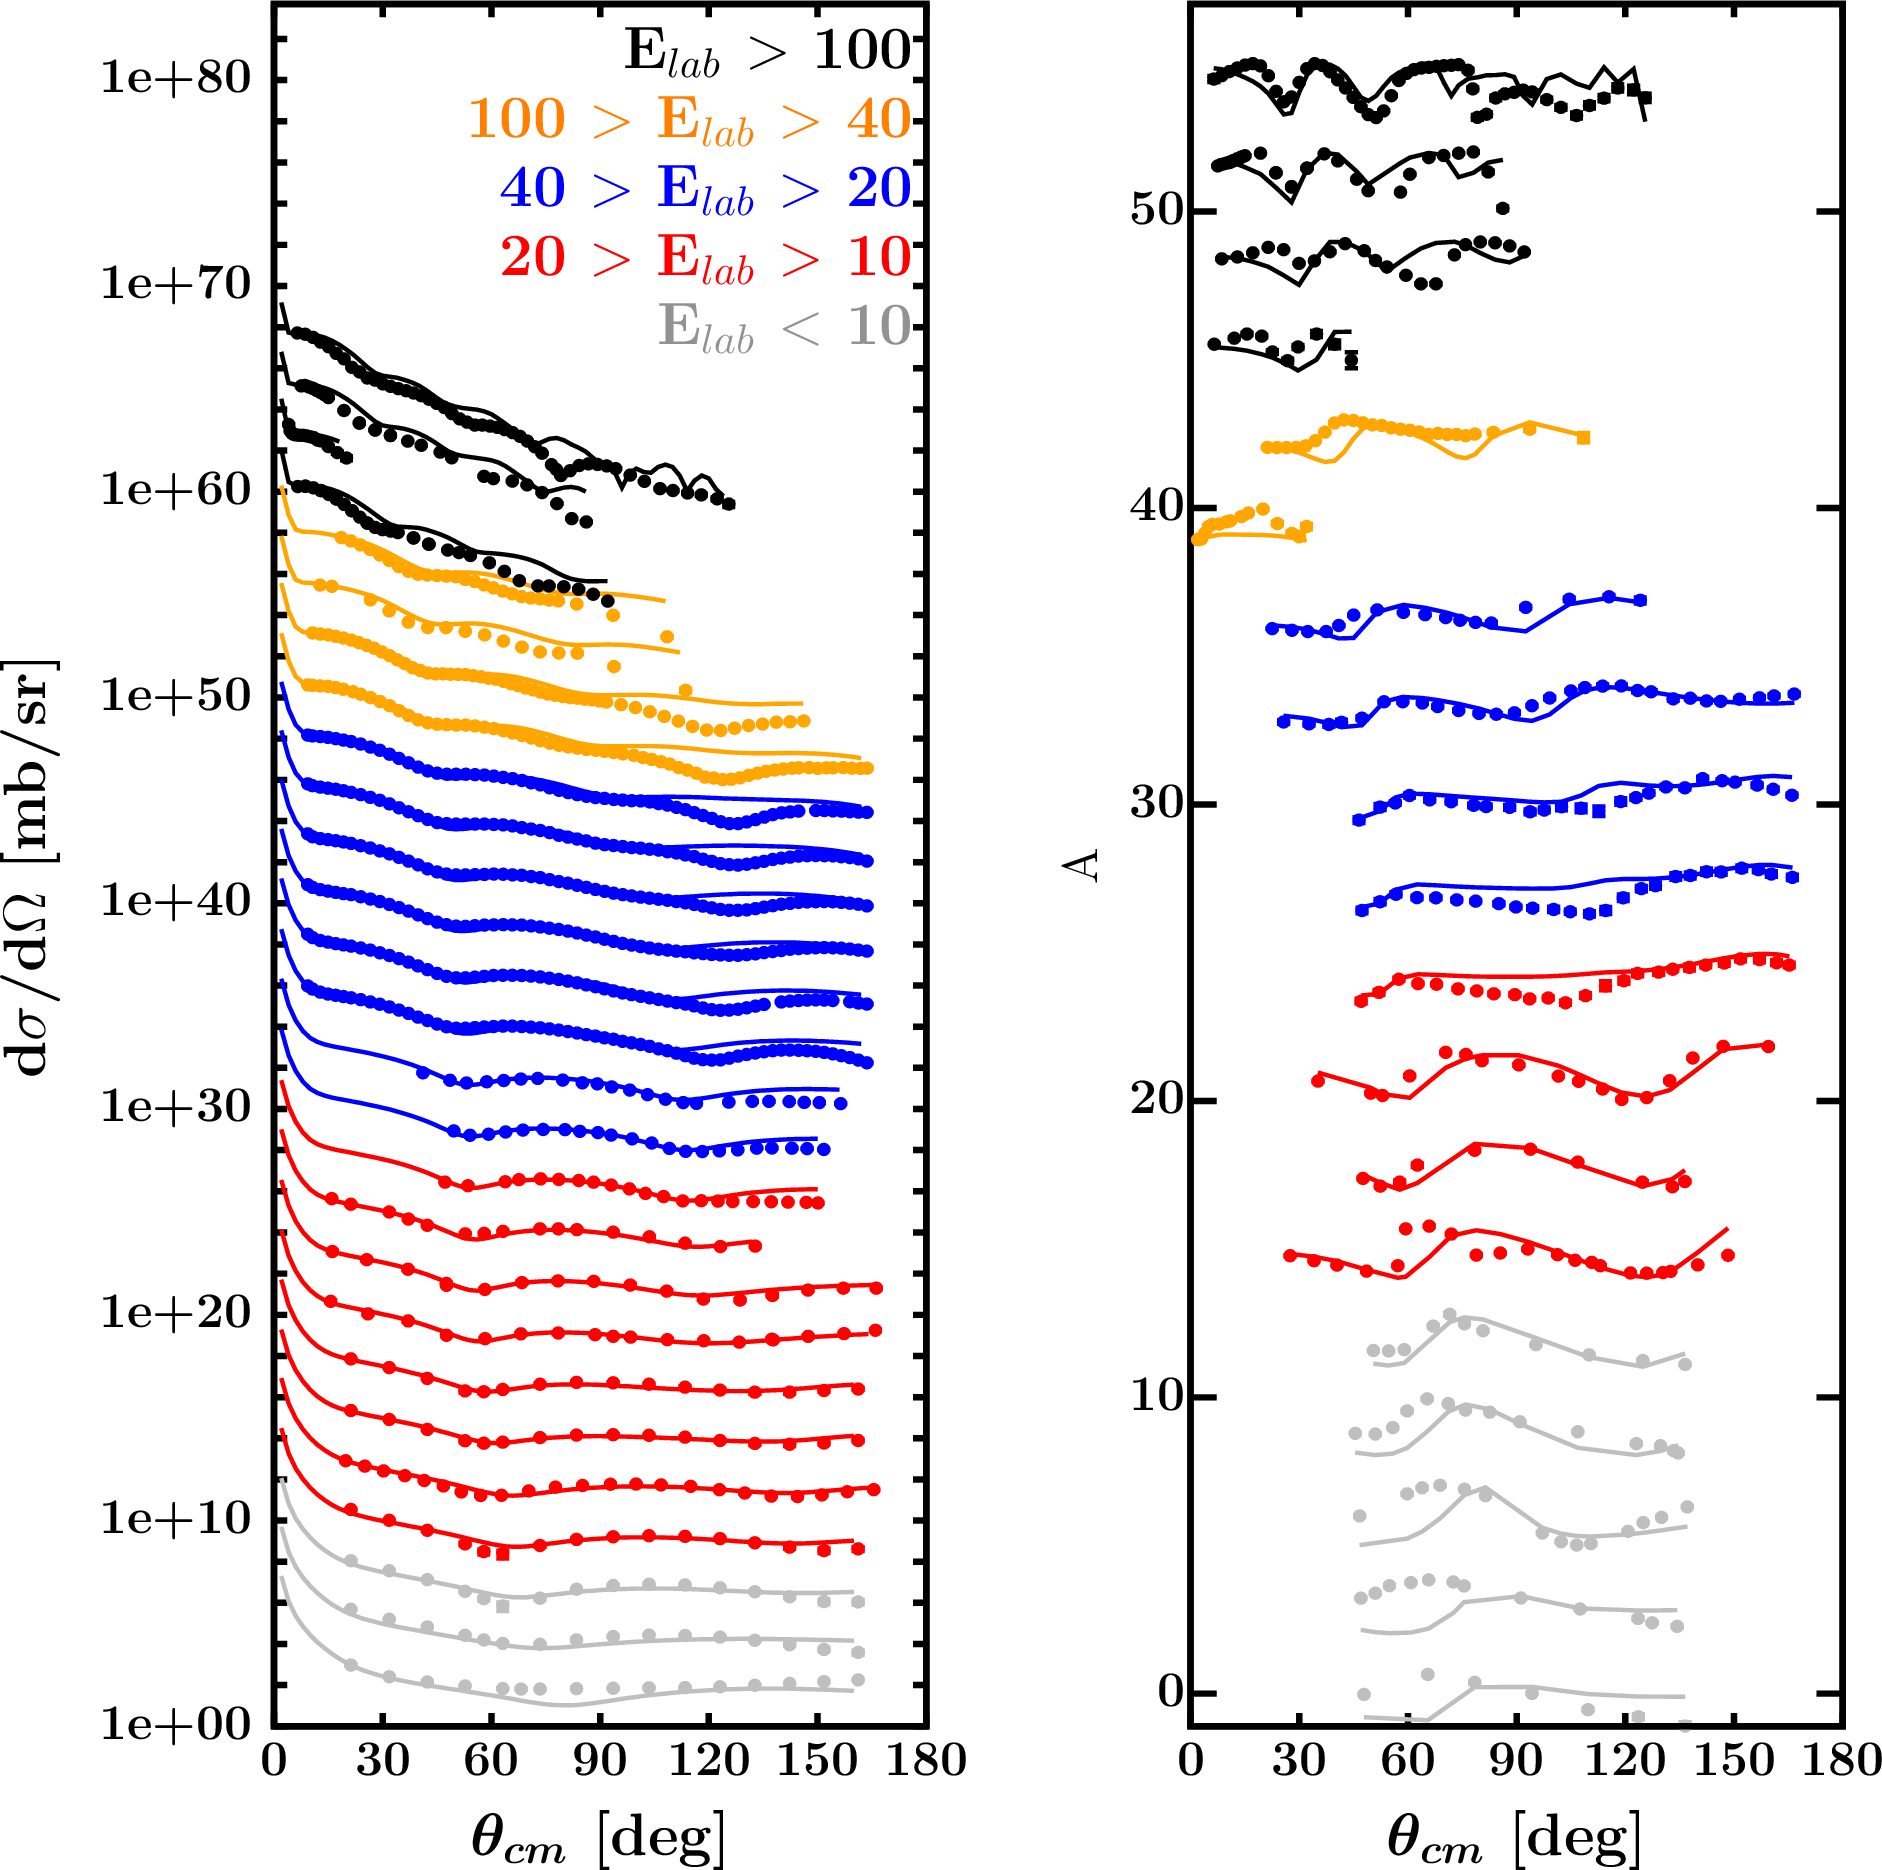
\includegraphics[width=\textwidth]{figures/o16_protonElastic.png}
        \caption*{\oSix\ proton elastic scattering}
        \label{DOMFitData_o16_proton_elastic}
    \end{minipage}\hspace{6pt}
    \begin{minipage}{0.47\textwidth}
        \centering
        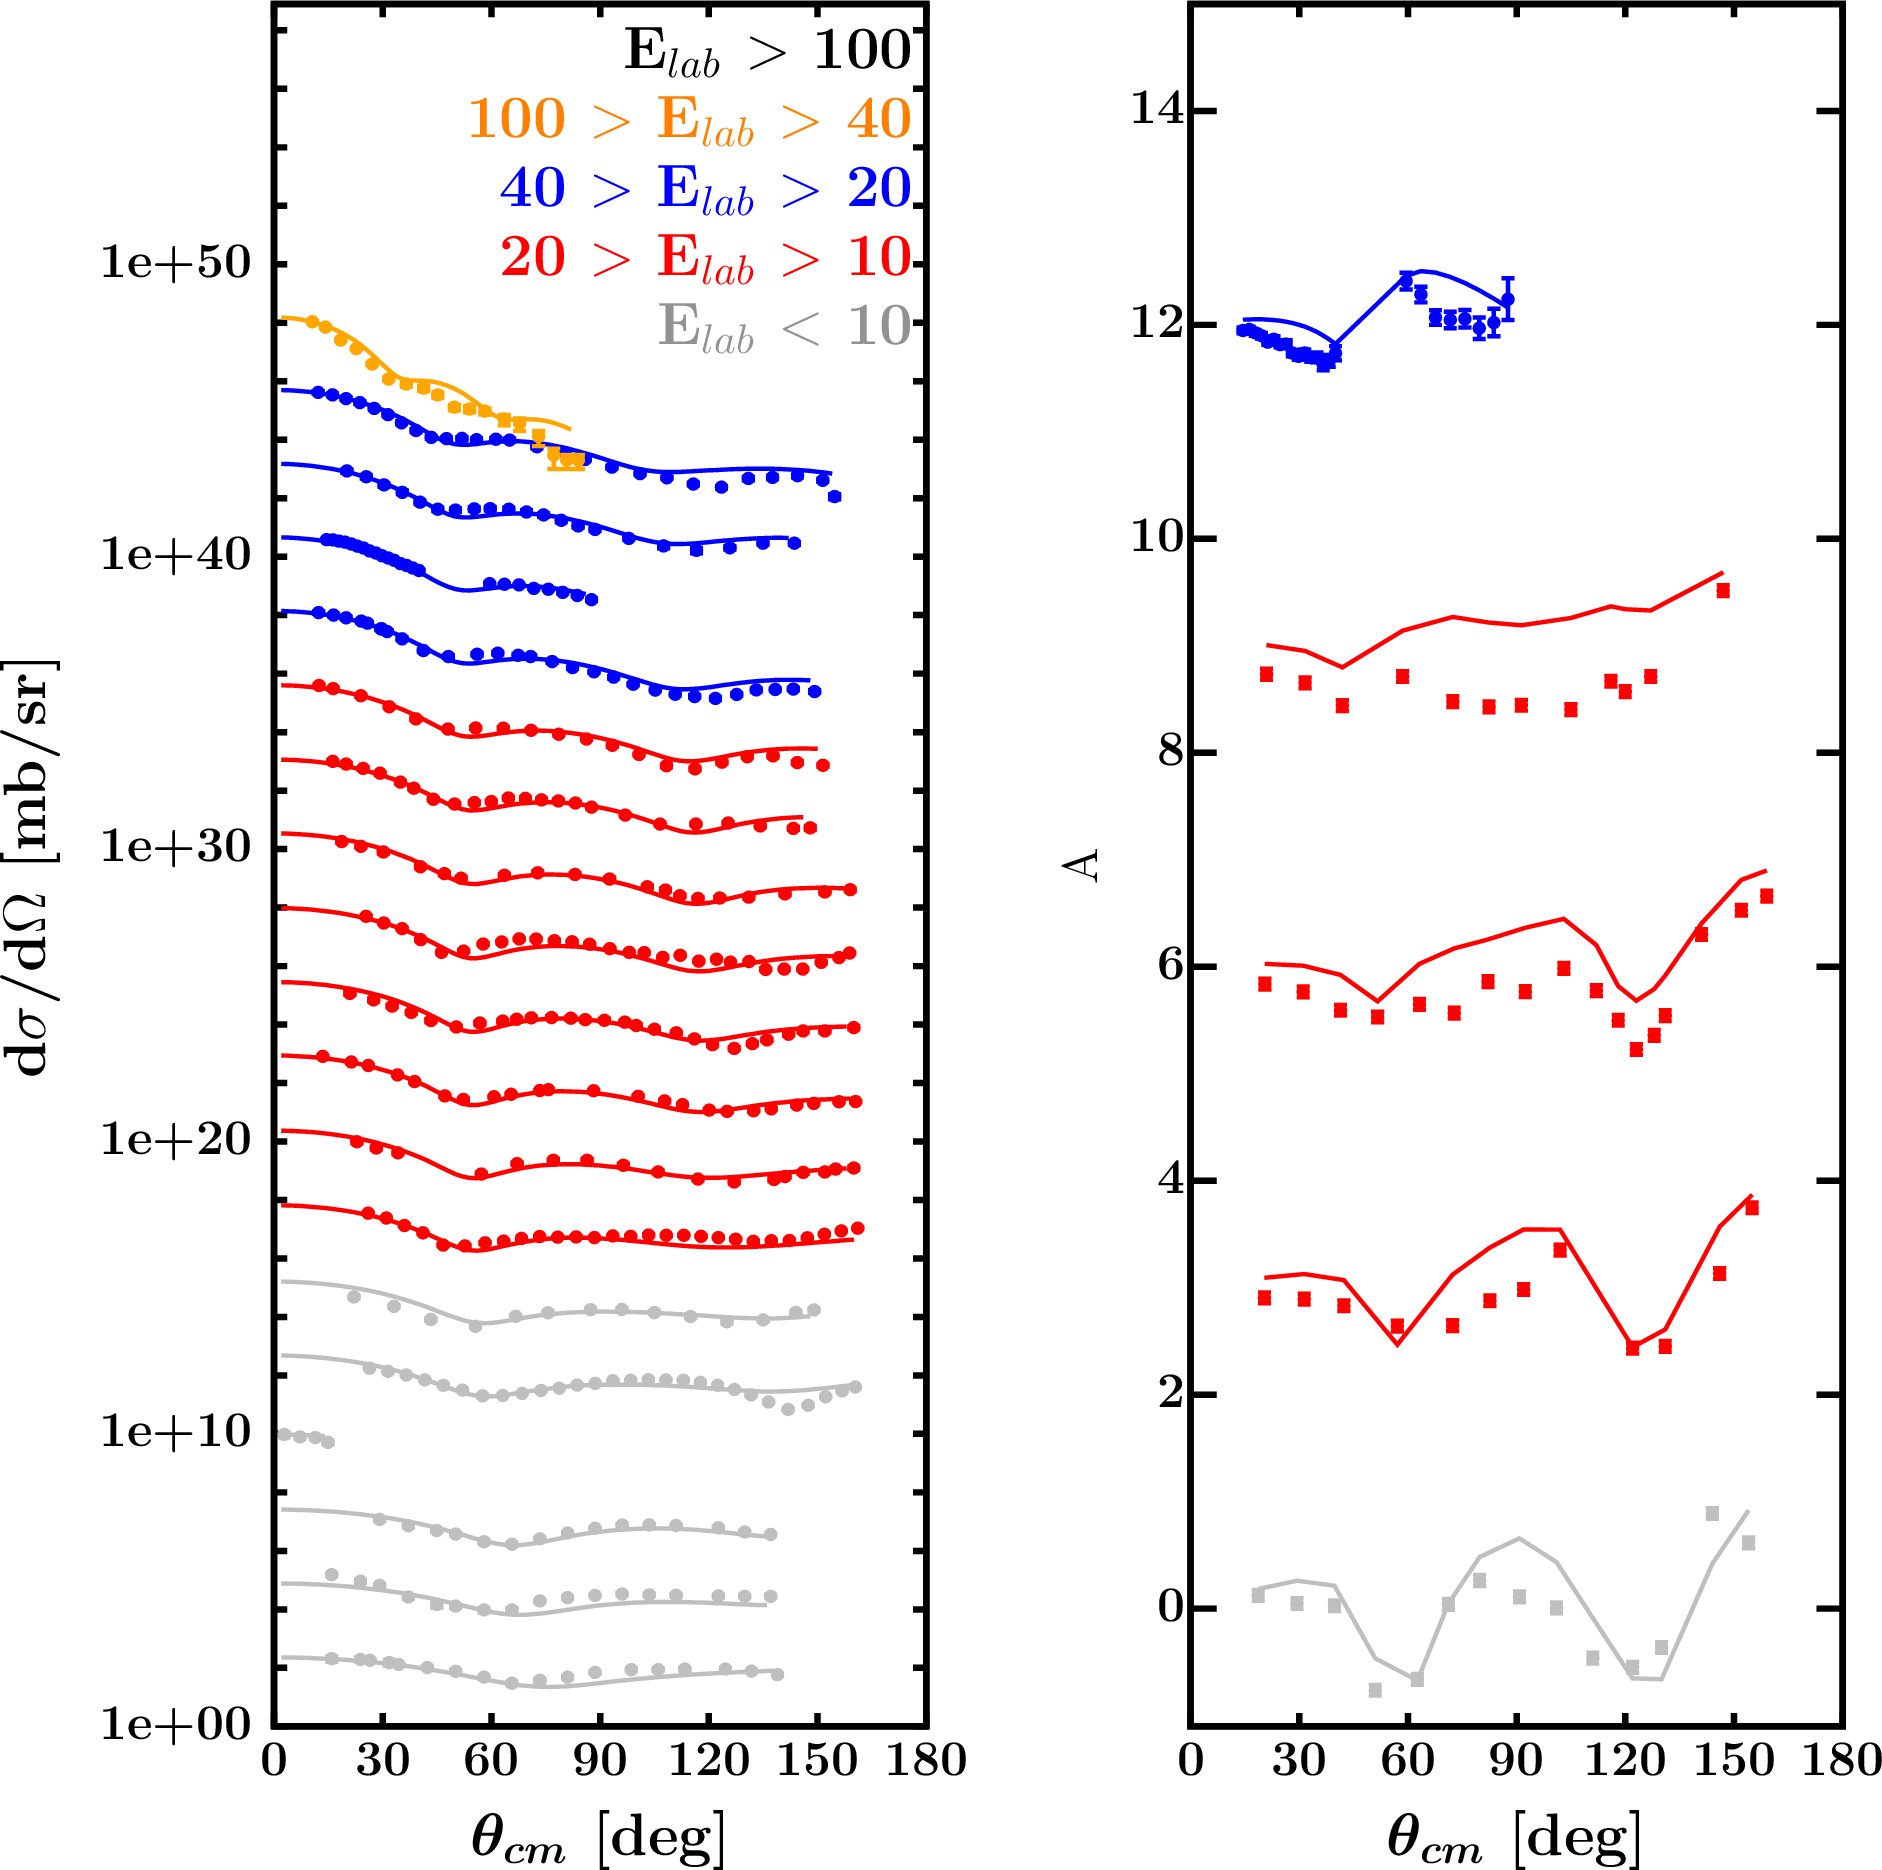
\includegraphics[width=\textwidth]{figures/o16_neutronElastic.png}
        \caption*{\oSix\ neutron elastic scattering}
        \label{DOMFitData_o16_neutron_elastic}
    \end{minipage}
\end{figure}
\vspace{0.70in}
\begin{figure}[hbtp]
    \centering
    \begin{minipage}{0.47\textwidth}
        \centering
        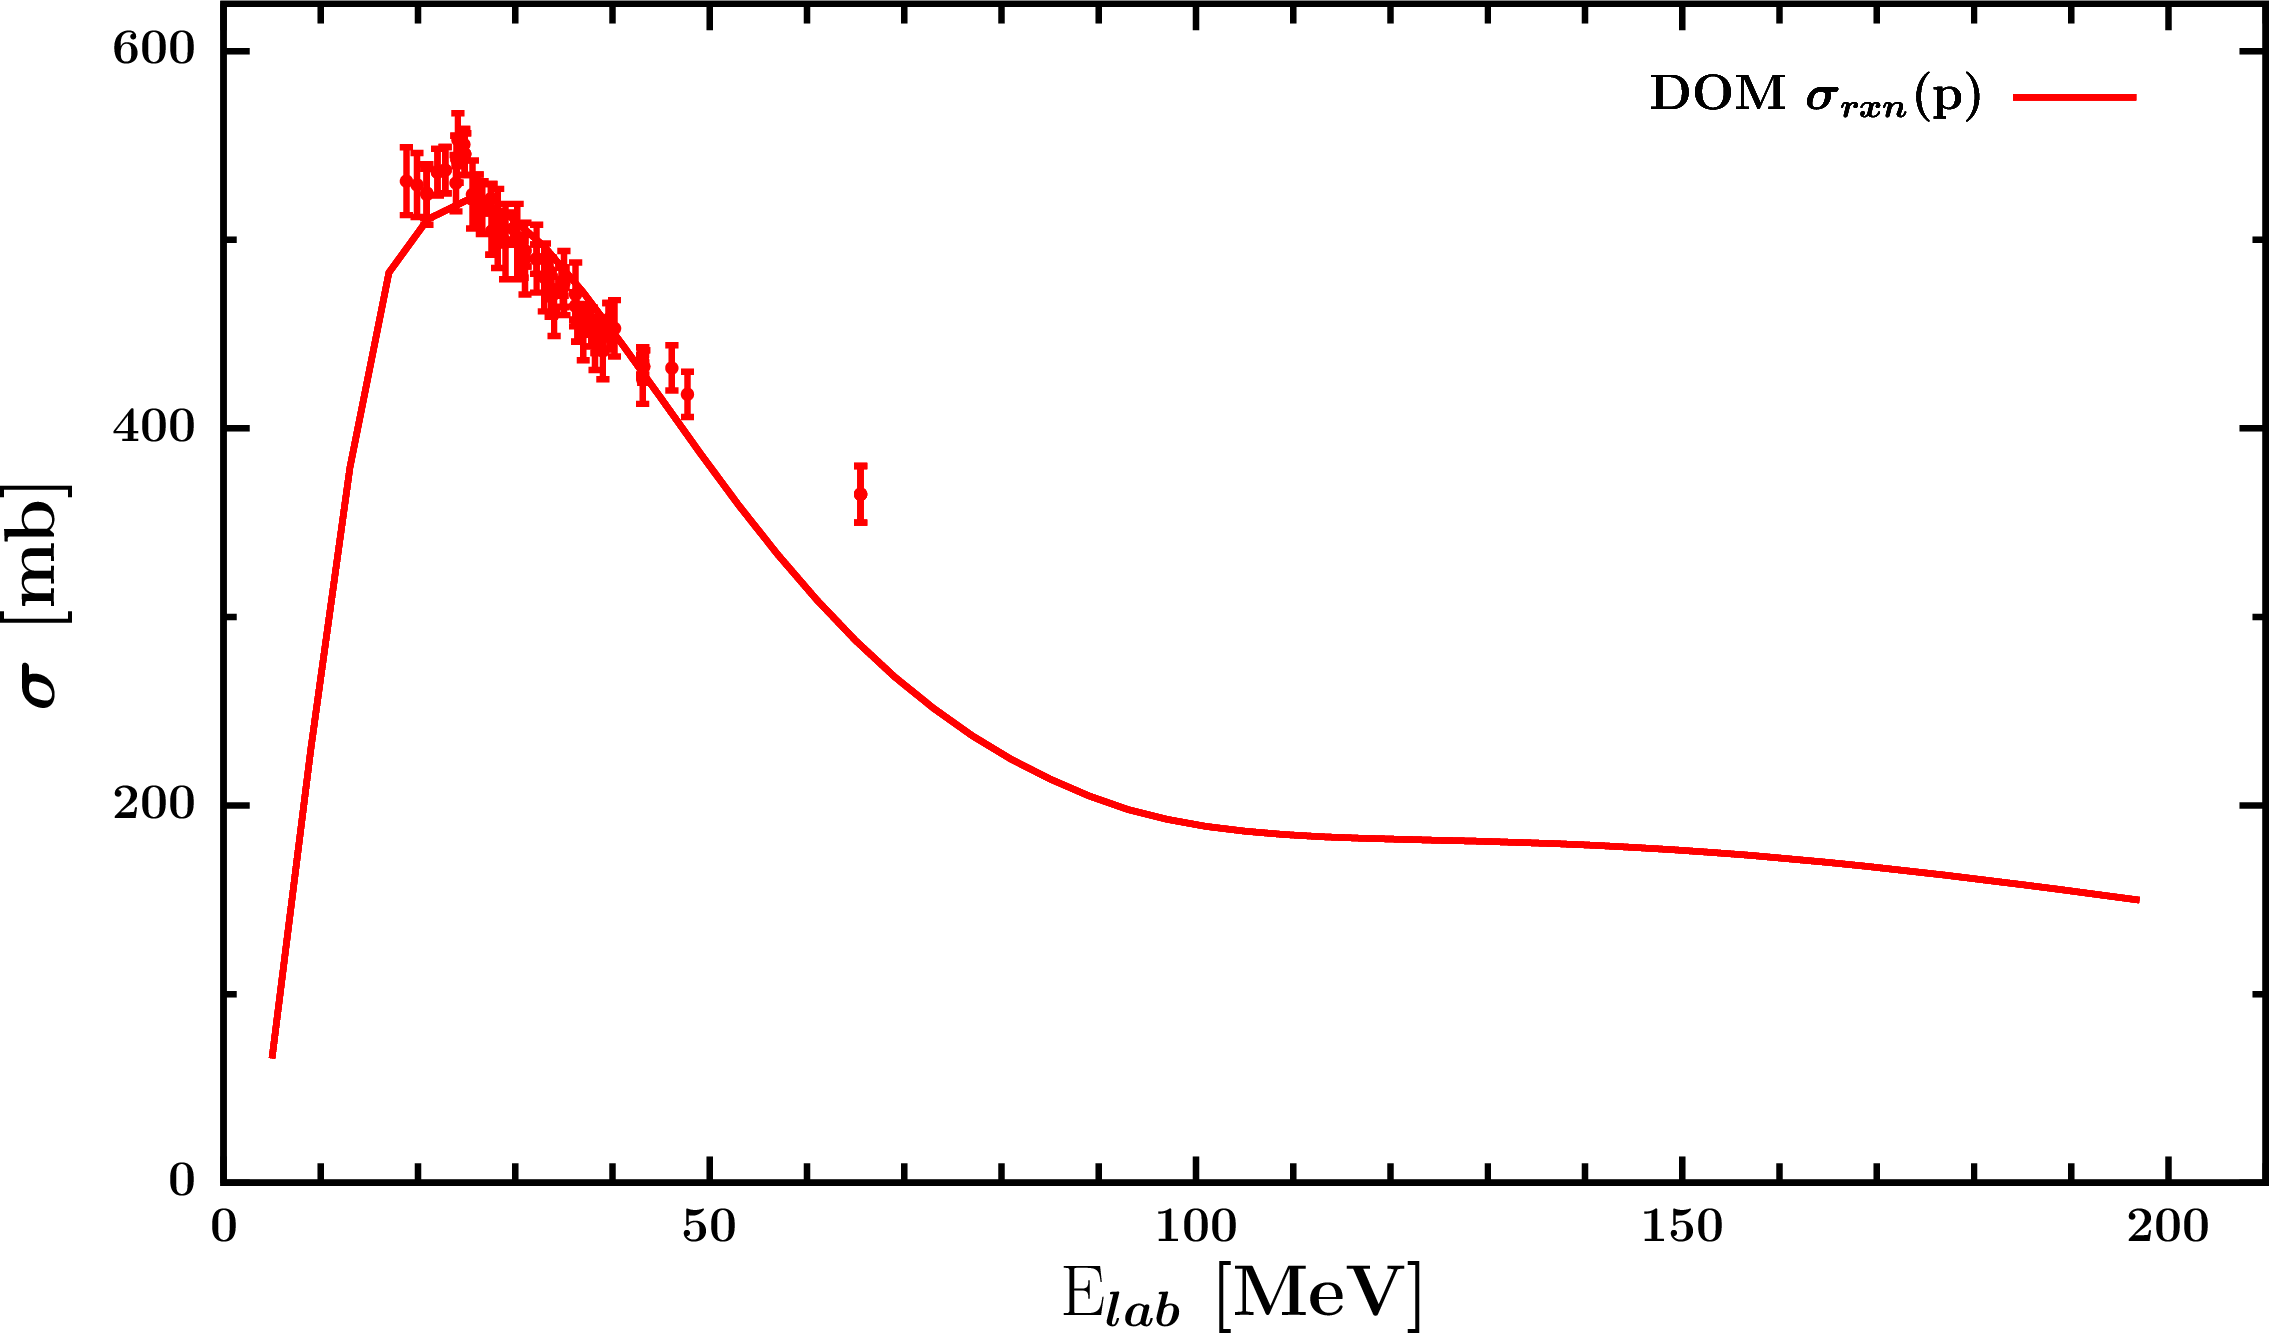
\includegraphics[width=\linewidth]{figures/o16_protonInelastic.png}
        \caption*{\oSix\ proton \rxn}
        \label{DOMFitData_o16_proton_inelastic}
    \end{minipage}\hspace{6pt}
    \begin{minipage}{0.47\textwidth}
        \centering
        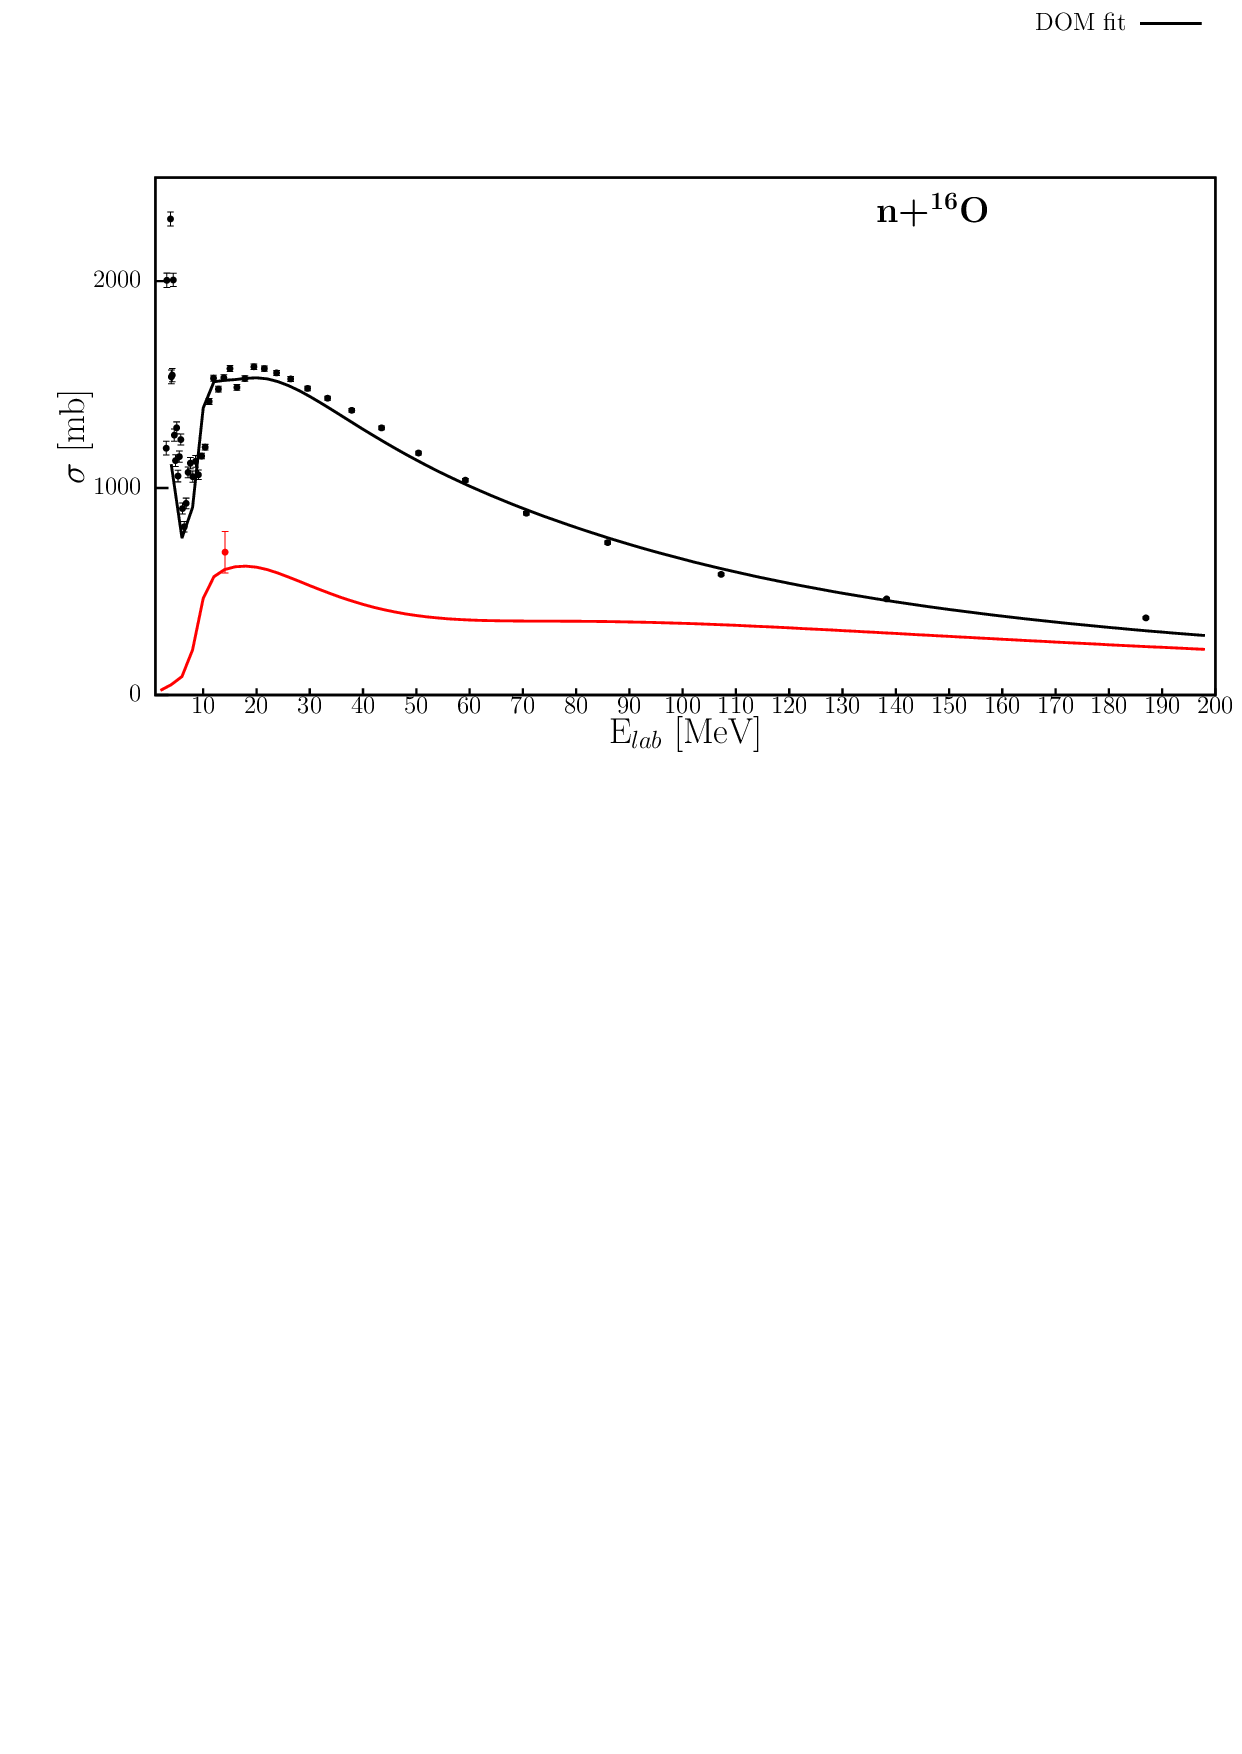
\includegraphics[width=\textwidth]{figures/o16_neutronInelastic.png}
        \caption*{\oSix\ neutron \rxn\ and \tot}
        \label{DOMFitData_o16_neutron_inelastic}
    \end{minipage}
\end{figure}
%\afterpage{\clearpage}
\begin{figure}[hbtp]
    \centering
    \begin{minipage}{0.42\textwidth}
        \centering
        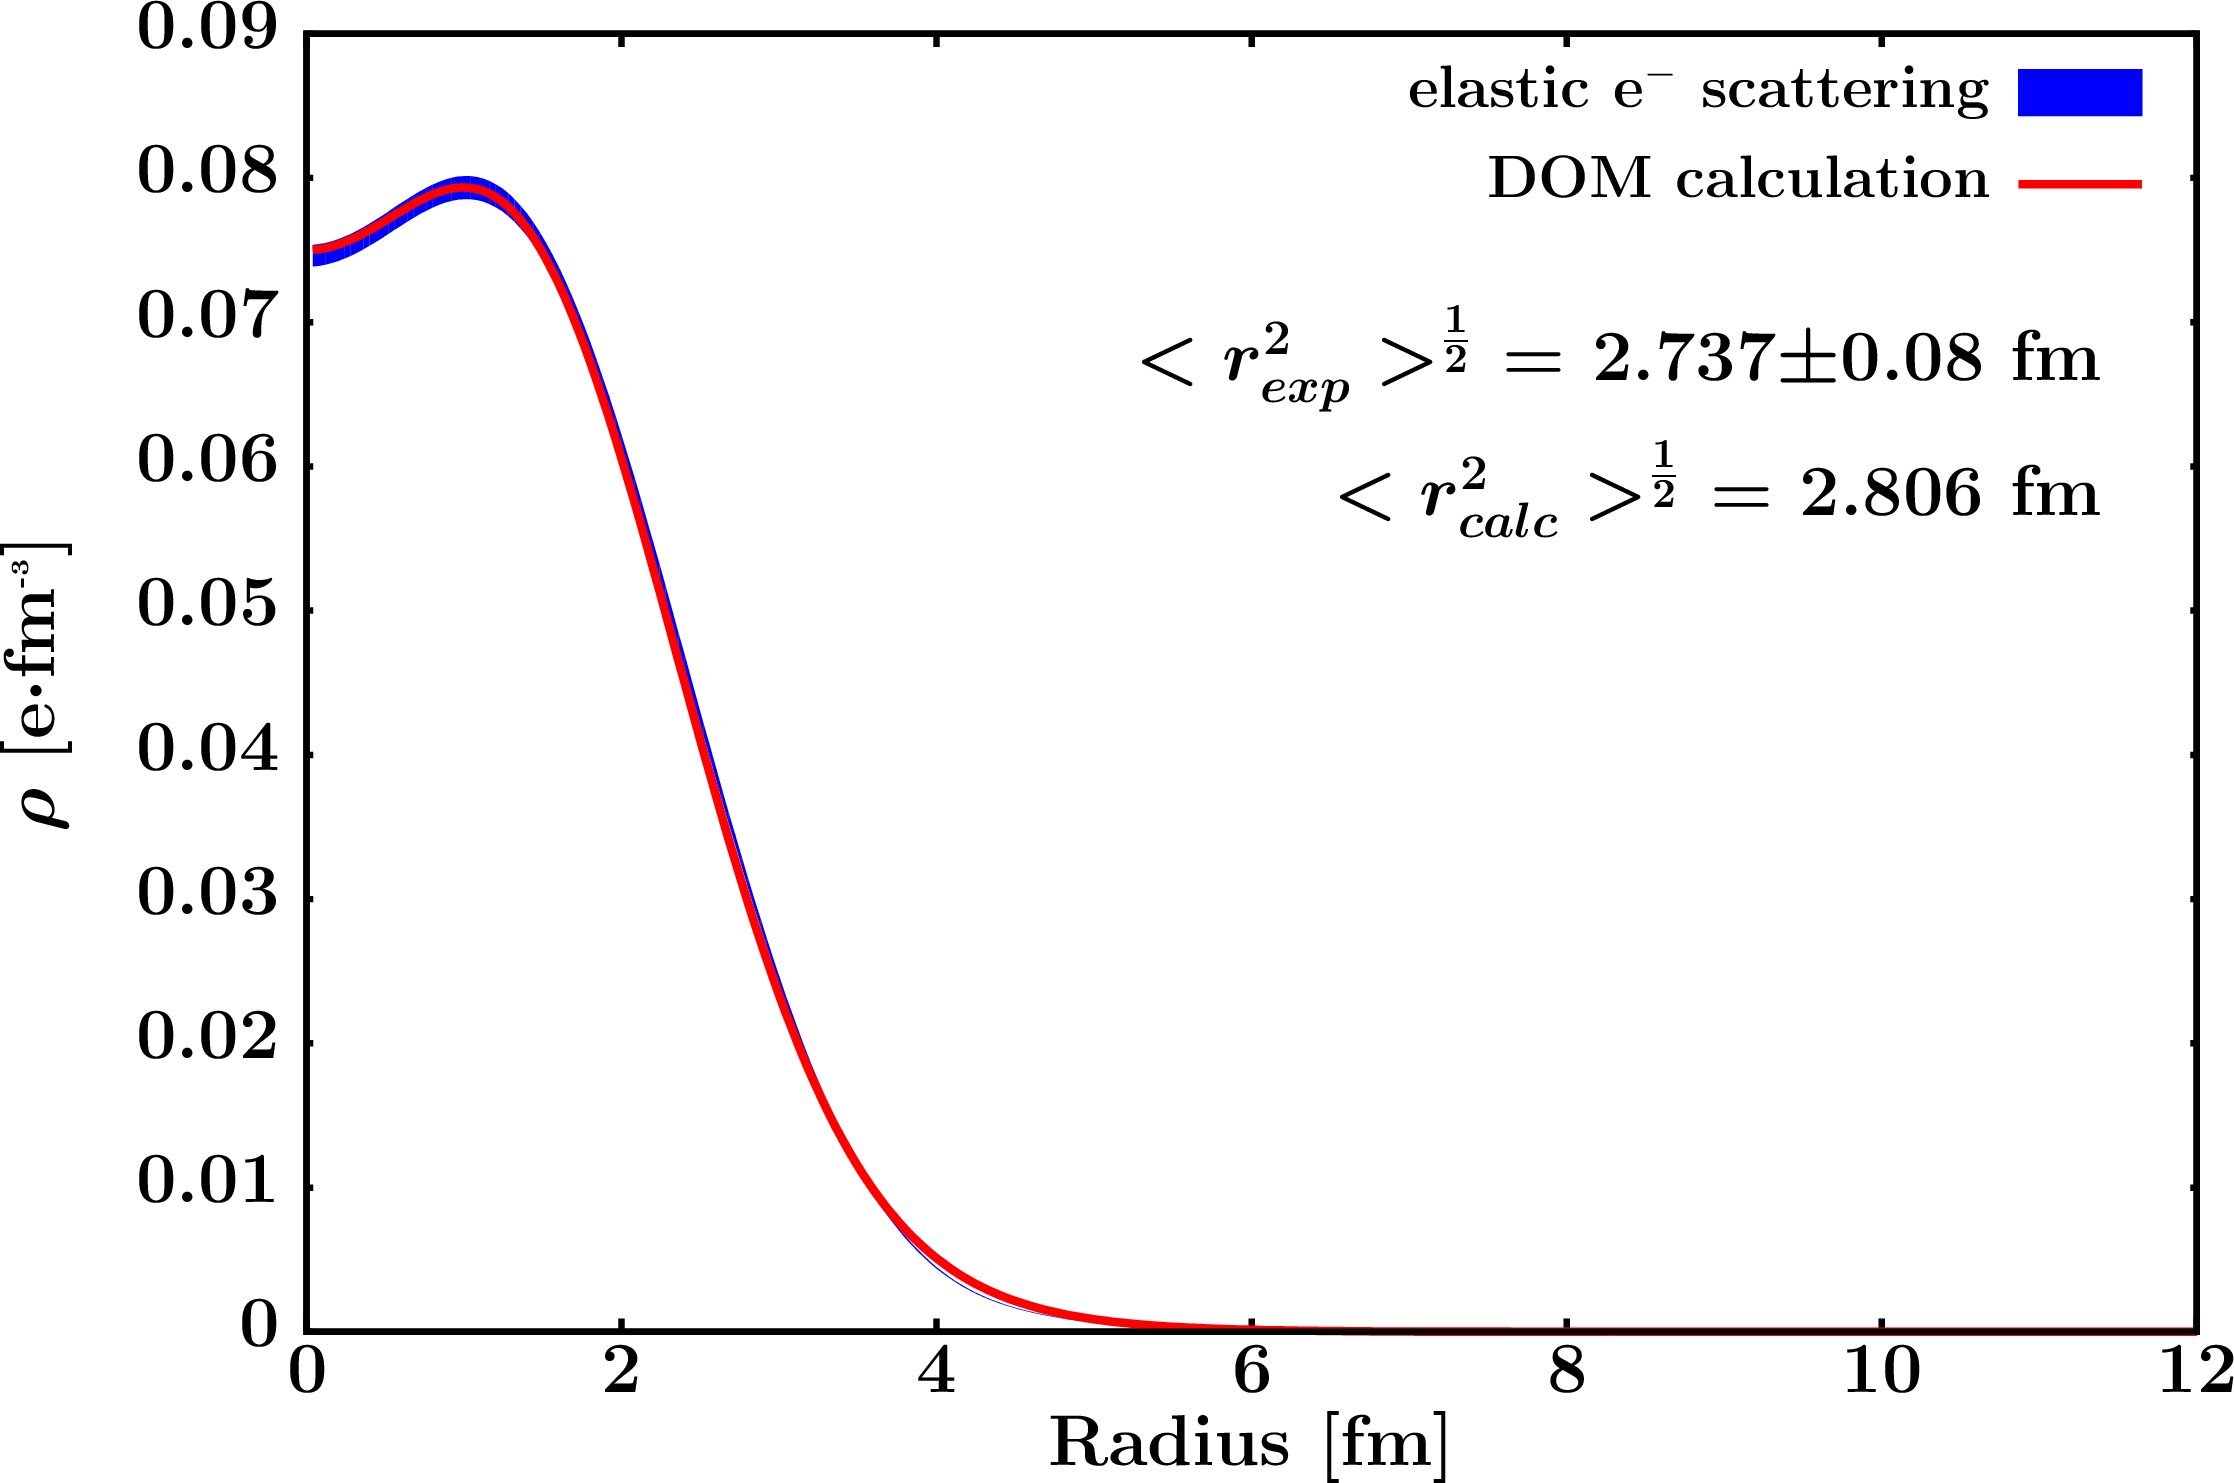
\includegraphics[width=\textwidth]{figures/o16_chargeDensity.png}
        \caption*{\oSix\ charge density}
        \label{DOMFitData_o16_chargeDensity}
    \end{minipage}\hspace{6pt}
    \begin{minipage}{0.42\textwidth}
        \centering
        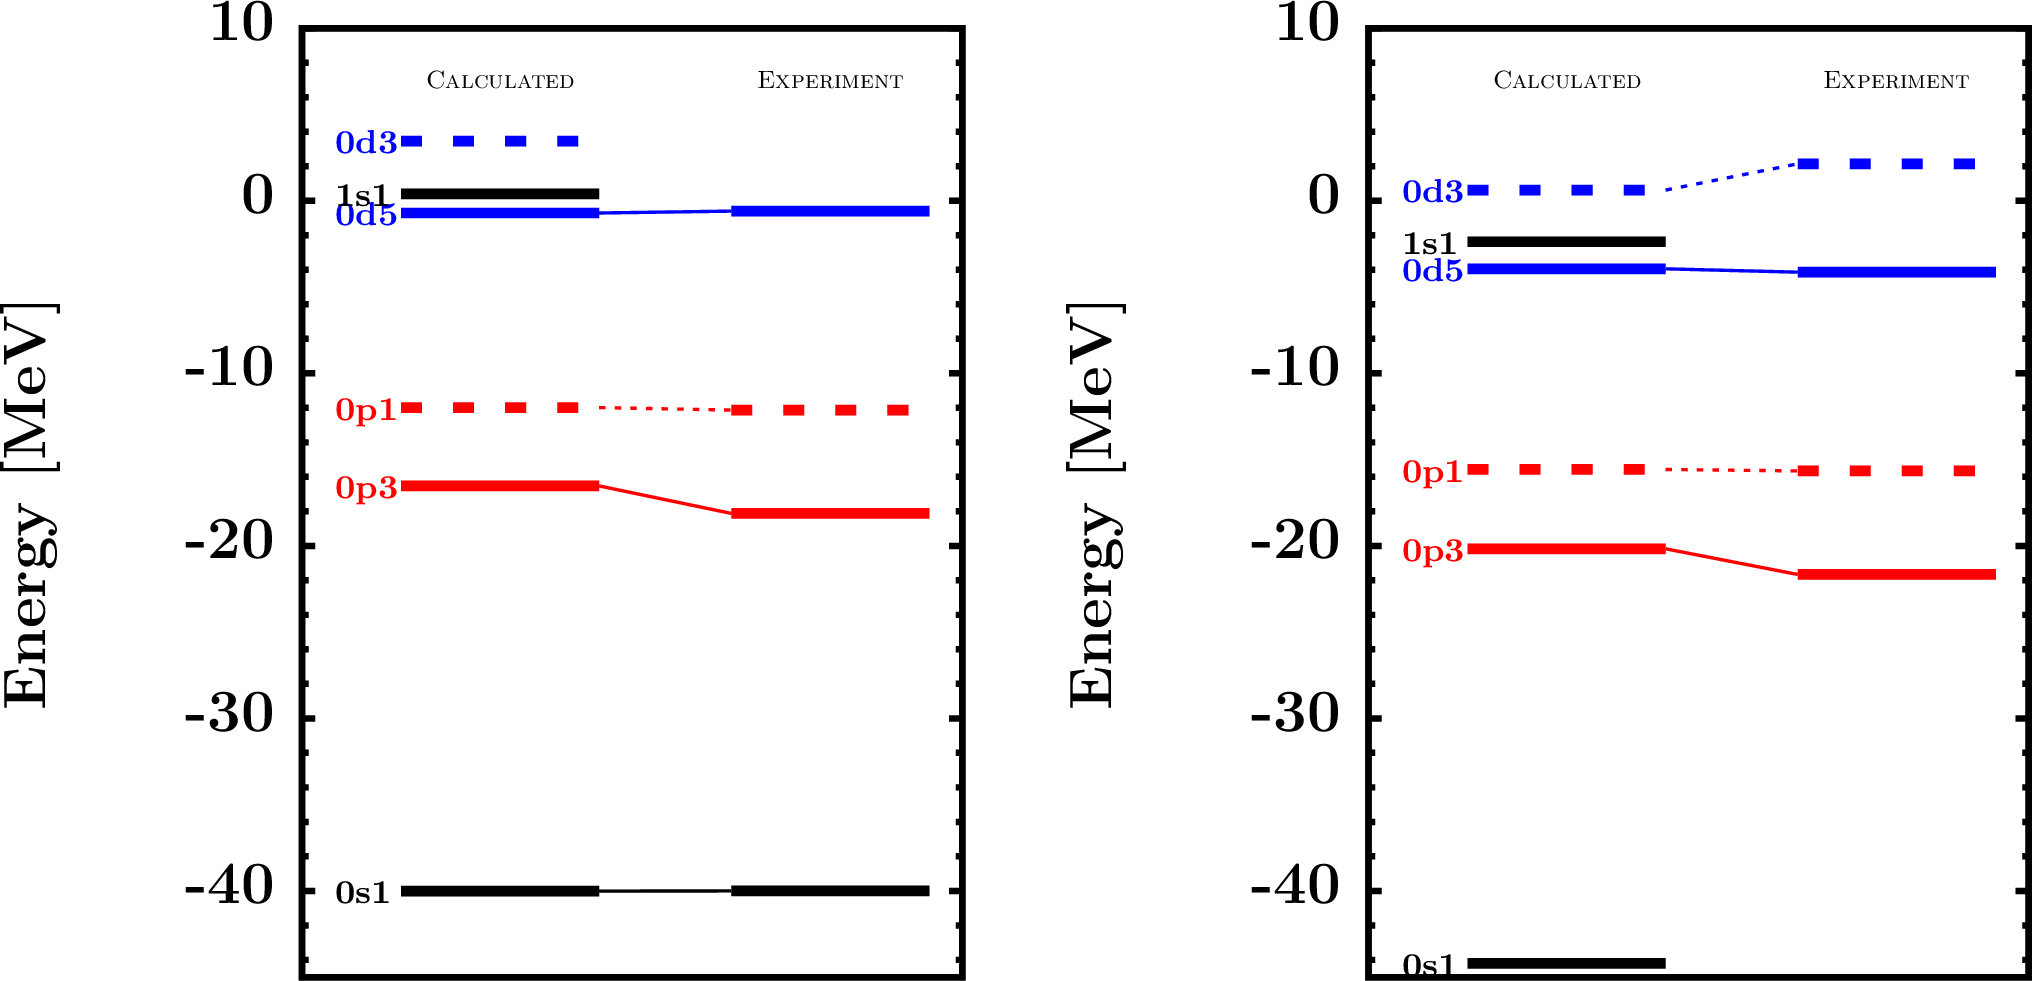
\includegraphics[width=\textwidth]{figures/o16_SPLevels.png}
        \caption*{\oSix\ single-particle levels}
        \label{DOMFitData_o16_SPLevels}
    \end{minipage}
\end{figure}
%\vspace{0.3in}
\begin{figure}[hbtp]
    \centering
    \begin{minipage}{0.42\textwidth}
        \centering
        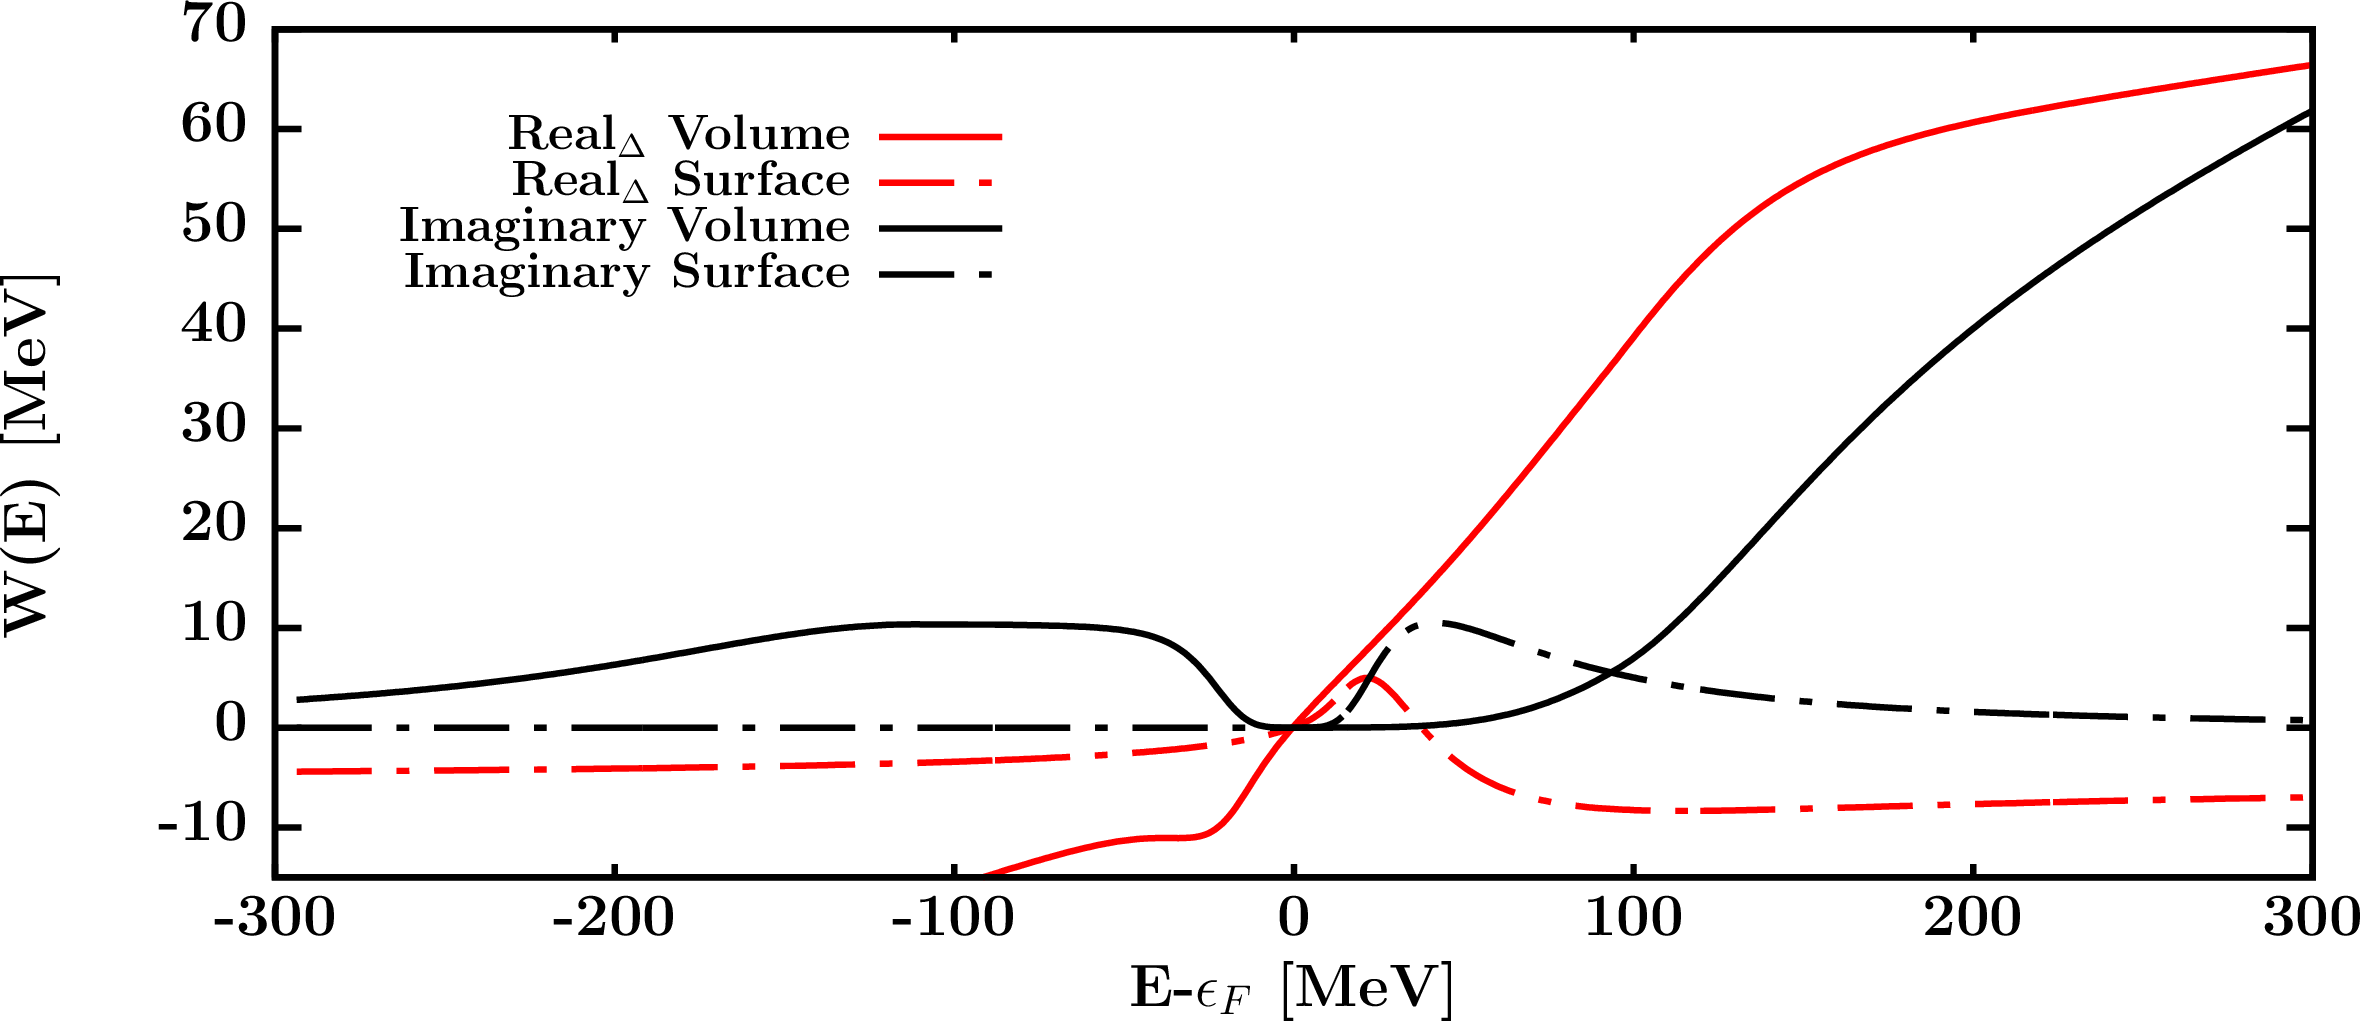
\includegraphics[width=\textwidth]{figures/o16_protonPotentials.png}
        \caption*{\footnotesize\oSix\ proton potential energy dependence}
        \label{DOMFitData_o16_proton_potentialComponent_energy}
    \end{minipage}\hspace{6pt}
    \begin{minipage}{0.42\textwidth}
        \centering
        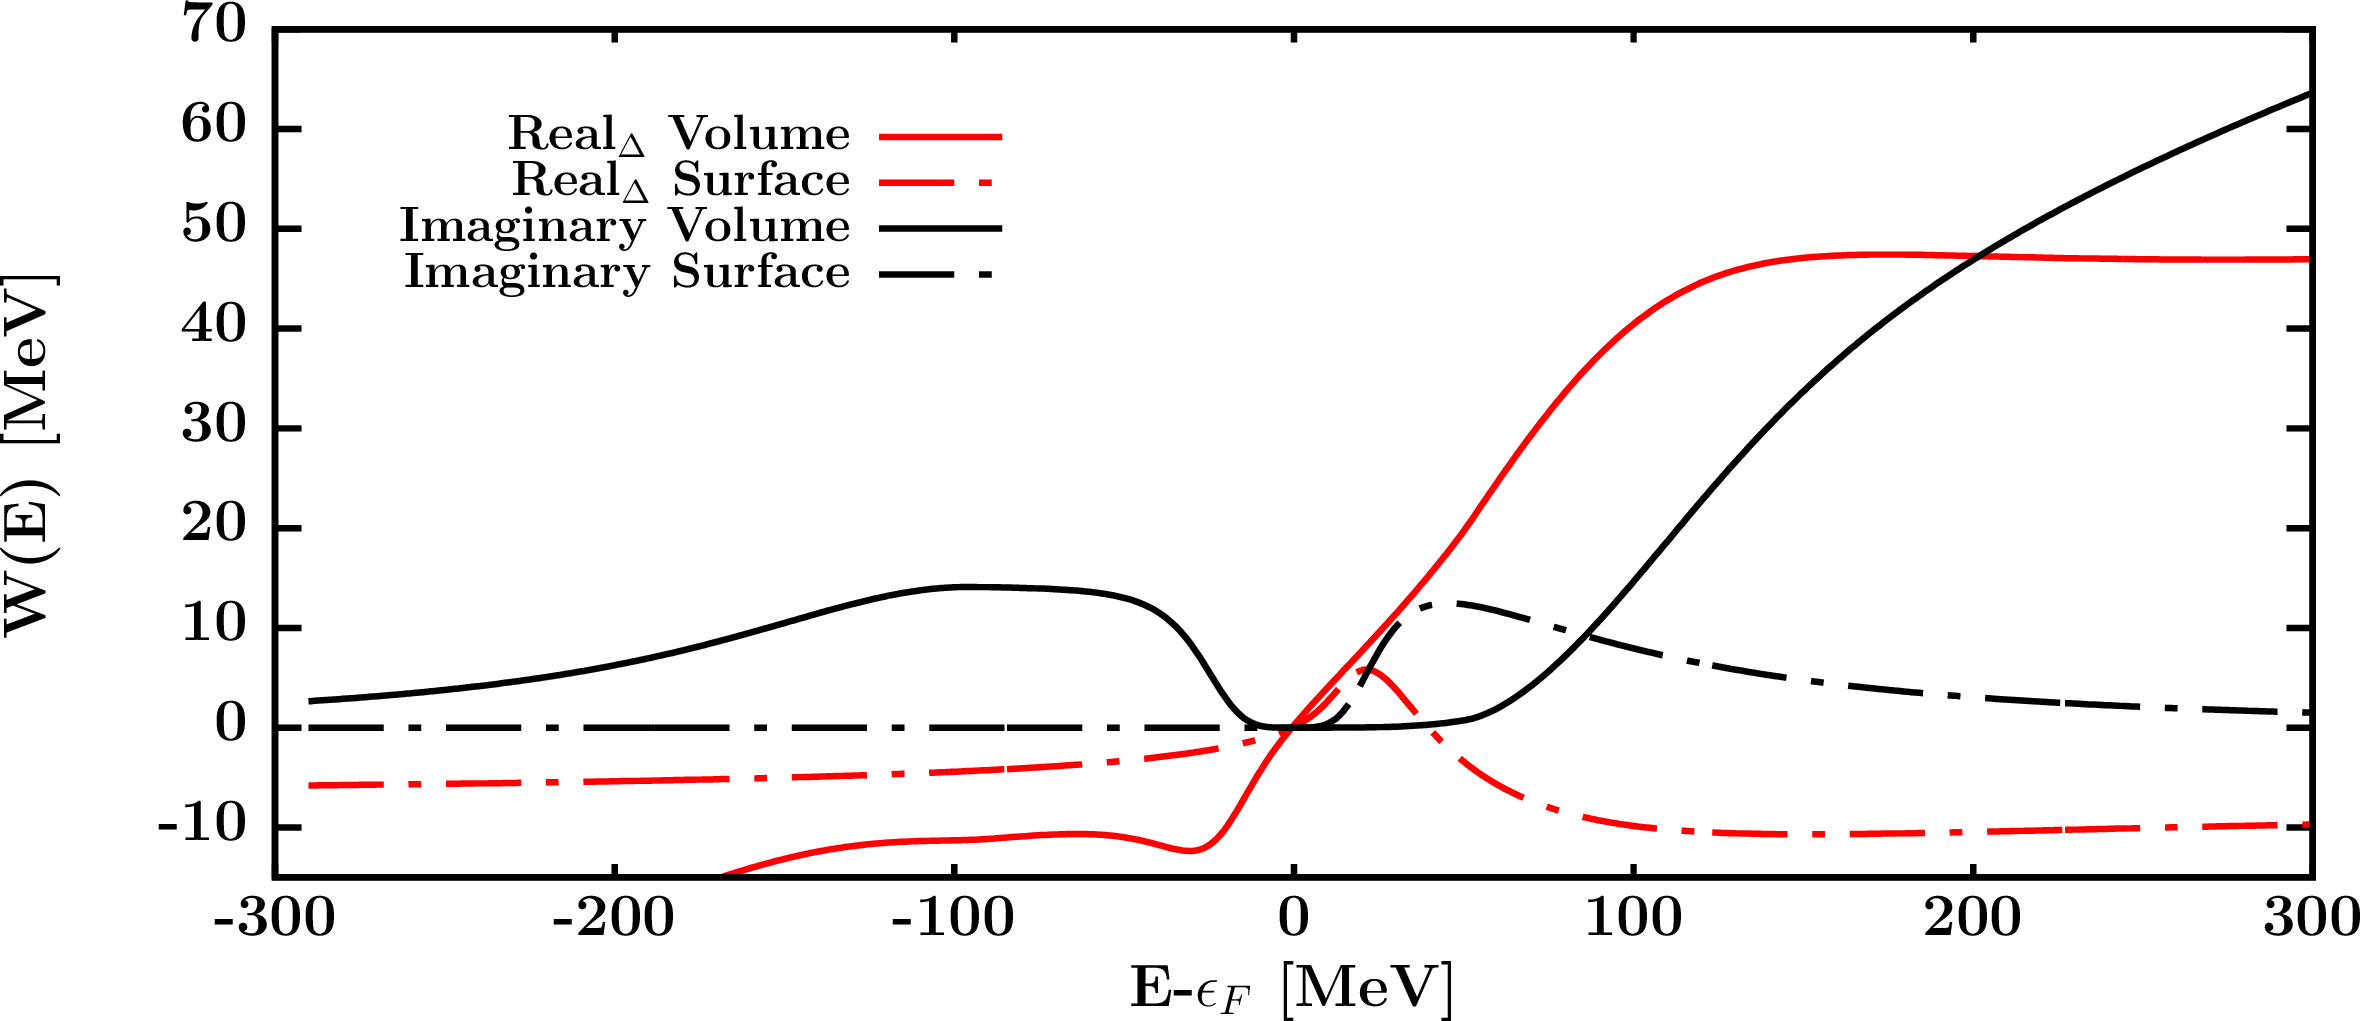
\includegraphics[width=\textwidth]{figures/o16_neutronPotentials.png}
        \caption*{\footnotesize\oSix\ neutron potential energy dependence}
        \label{DOMFitData_o16_neutron_potentialComponent_energy}
    \end{minipage}
\end{figure}
%\vspace{0.3in}
\begin{figure}[hbtp]
    \centering
    \begin{minipage}{0.42\textwidth}
        \centering
        
\includegraphics[width=\textwidth]{figures/o16_protonVolumeIntegrals.png}
        \caption*{\oSix\ proton volume integral}
        \label{DOMFitData_o16_proton_potentialIntegral}
    \end{minipage}\hspace{6pt}
    \begin{minipage}{0.42\textwidth}
        \centering
        
\includegraphics[width=\textwidth]{figures/o16_neutronVolumeIntegrals.png}
        \caption*{\oSix\ neutron volume integral}
        \label{DOMFitData_o16_neutron_potentialIntegral}
    \end{minipage}
\end{figure}
%\vspace{0.3in}
\begin{figure}[hbtp]
    \centering
    \begin{minipage}{0.42\textwidth}
        \centering
        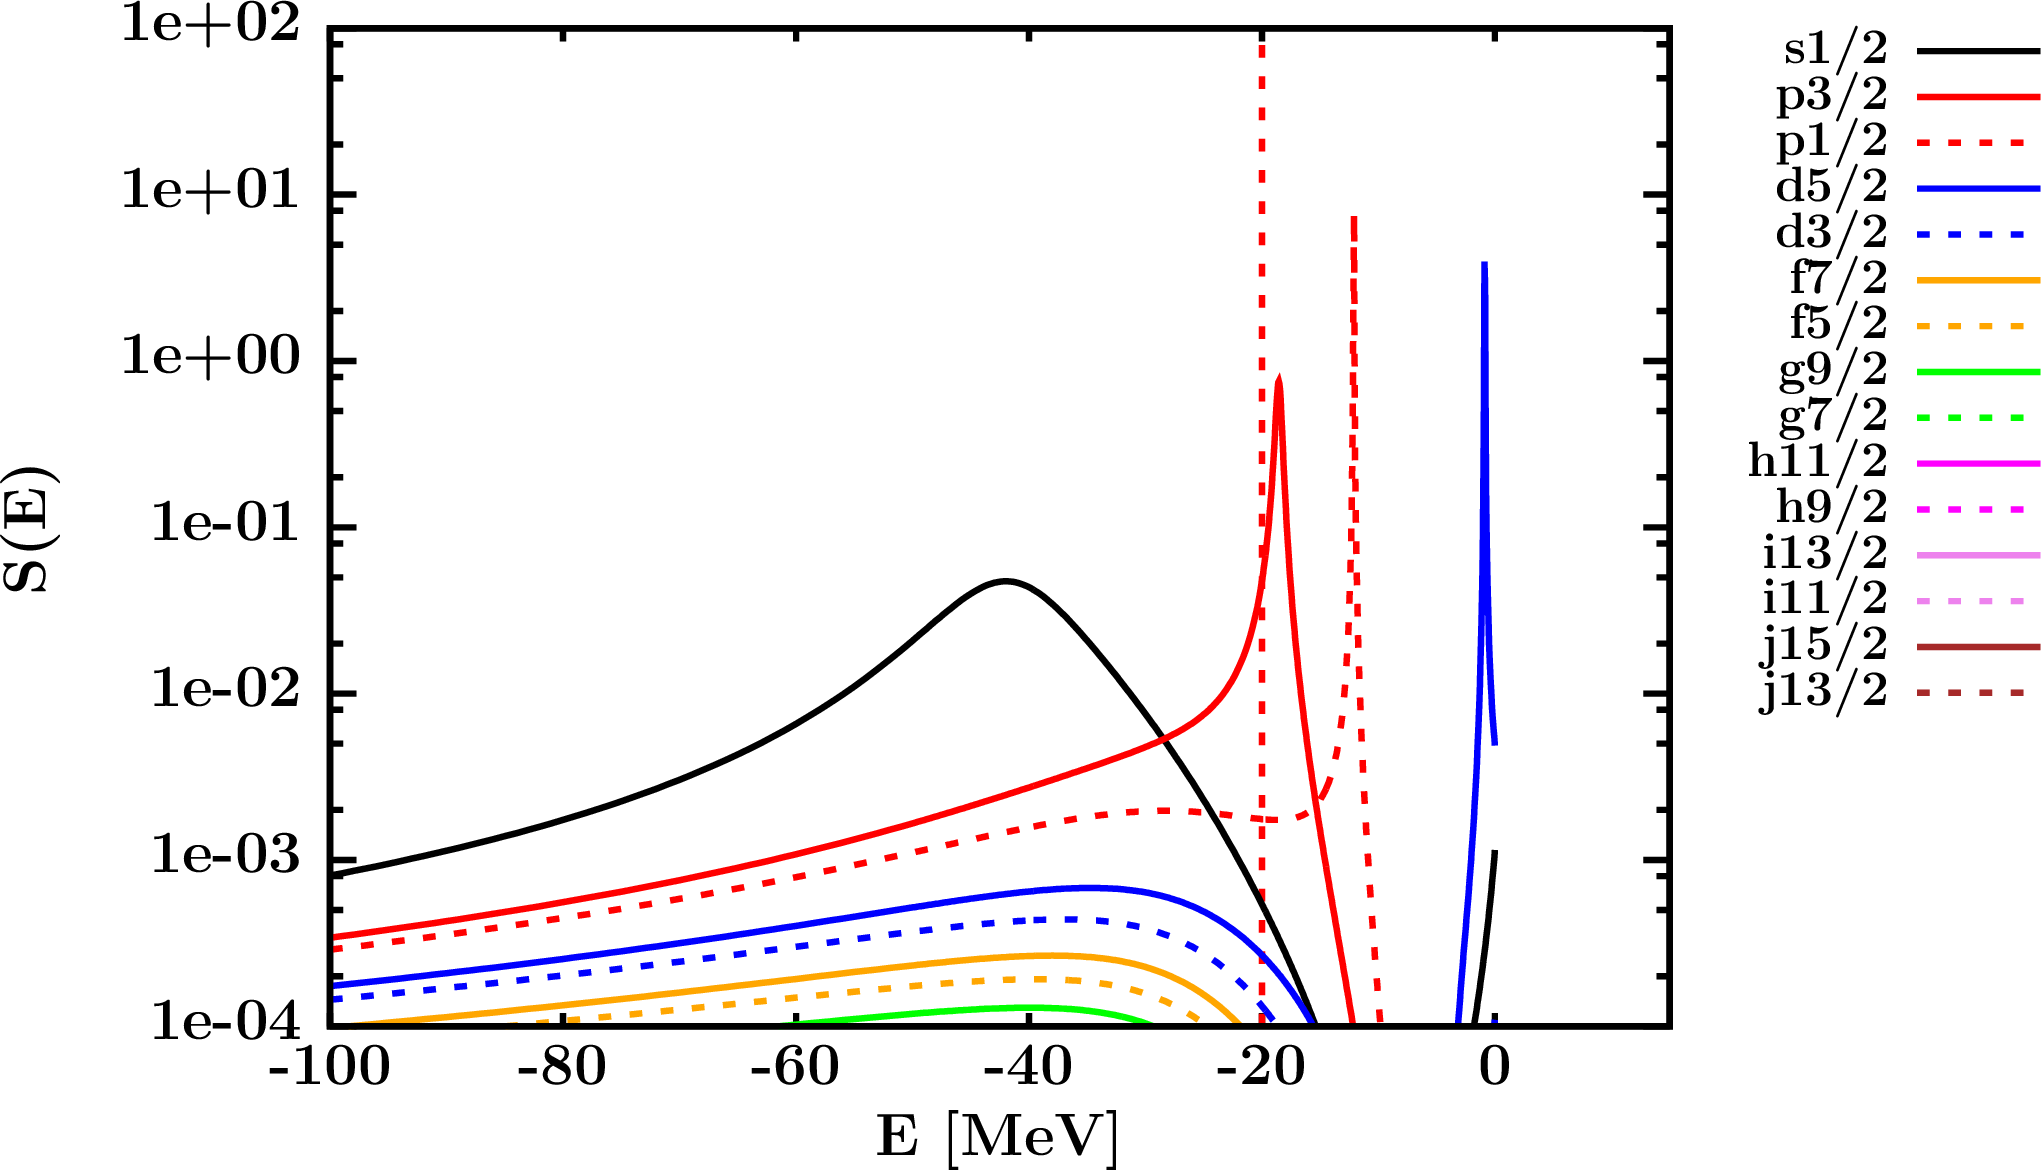
\includegraphics[width=\textwidth]{figures/o16_protonSpectralFunctions.png}
        \caption*{\oSix\ proton spectral functions}
        \label{DOMFitData_o16_proton_spectralFunctions}
    \end{minipage}\hspace{6pt}
    \begin{minipage}{0.42\textwidth}
        \centering
        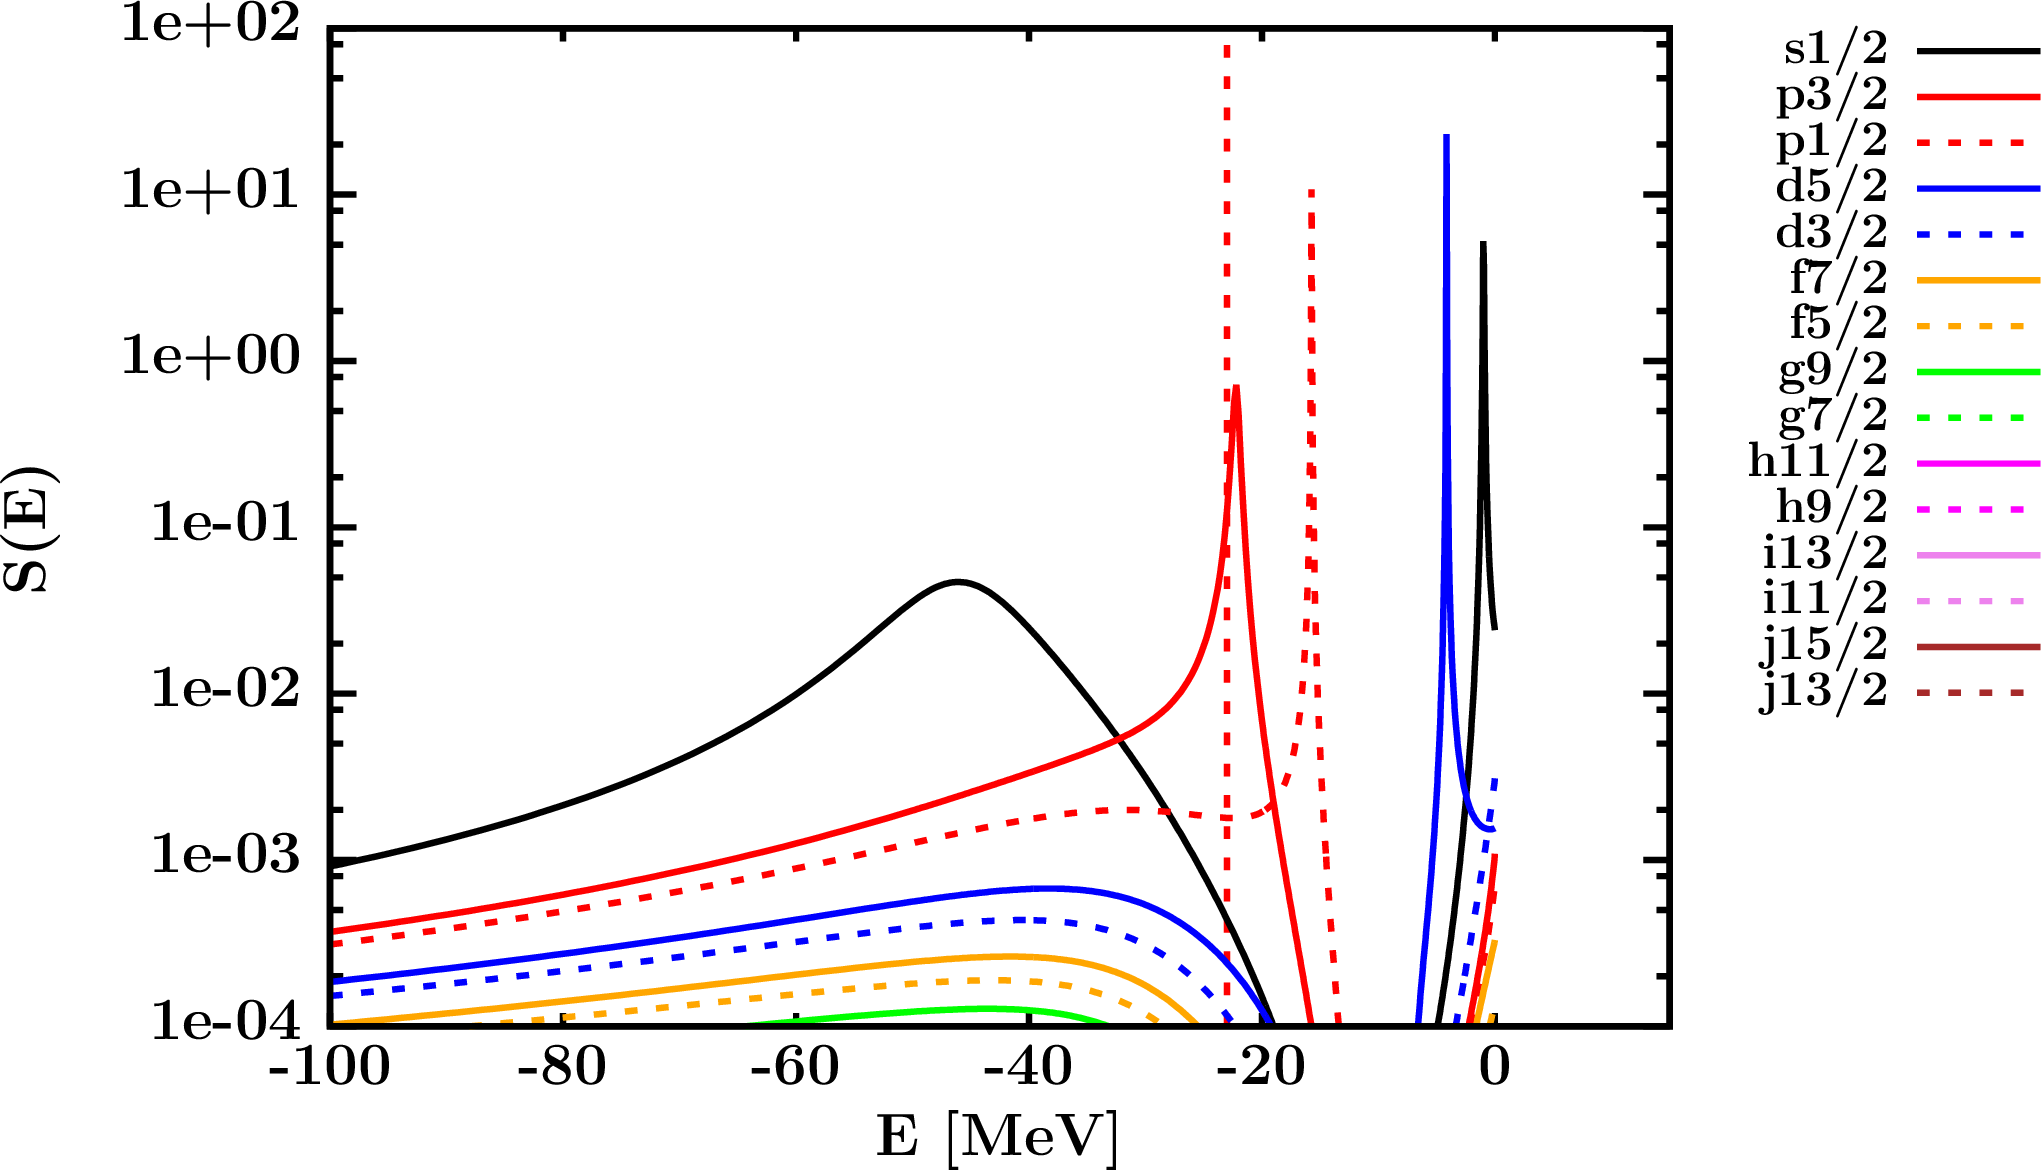
\includegraphics[width=\linewidth]{figures/o16_neutronSpectralFunctions.png}
        \caption*{\oSix\ neutron spectral functions}
        \label{DOMFitData_o16_neutron_spectralFunctions}
    \end{minipage}
\end{figure}
%\afterpage{\clearpage}
\begin{figure}[hbtp]
    \centering
    \begin{minipage}{0.45\textwidth}
        \centering
        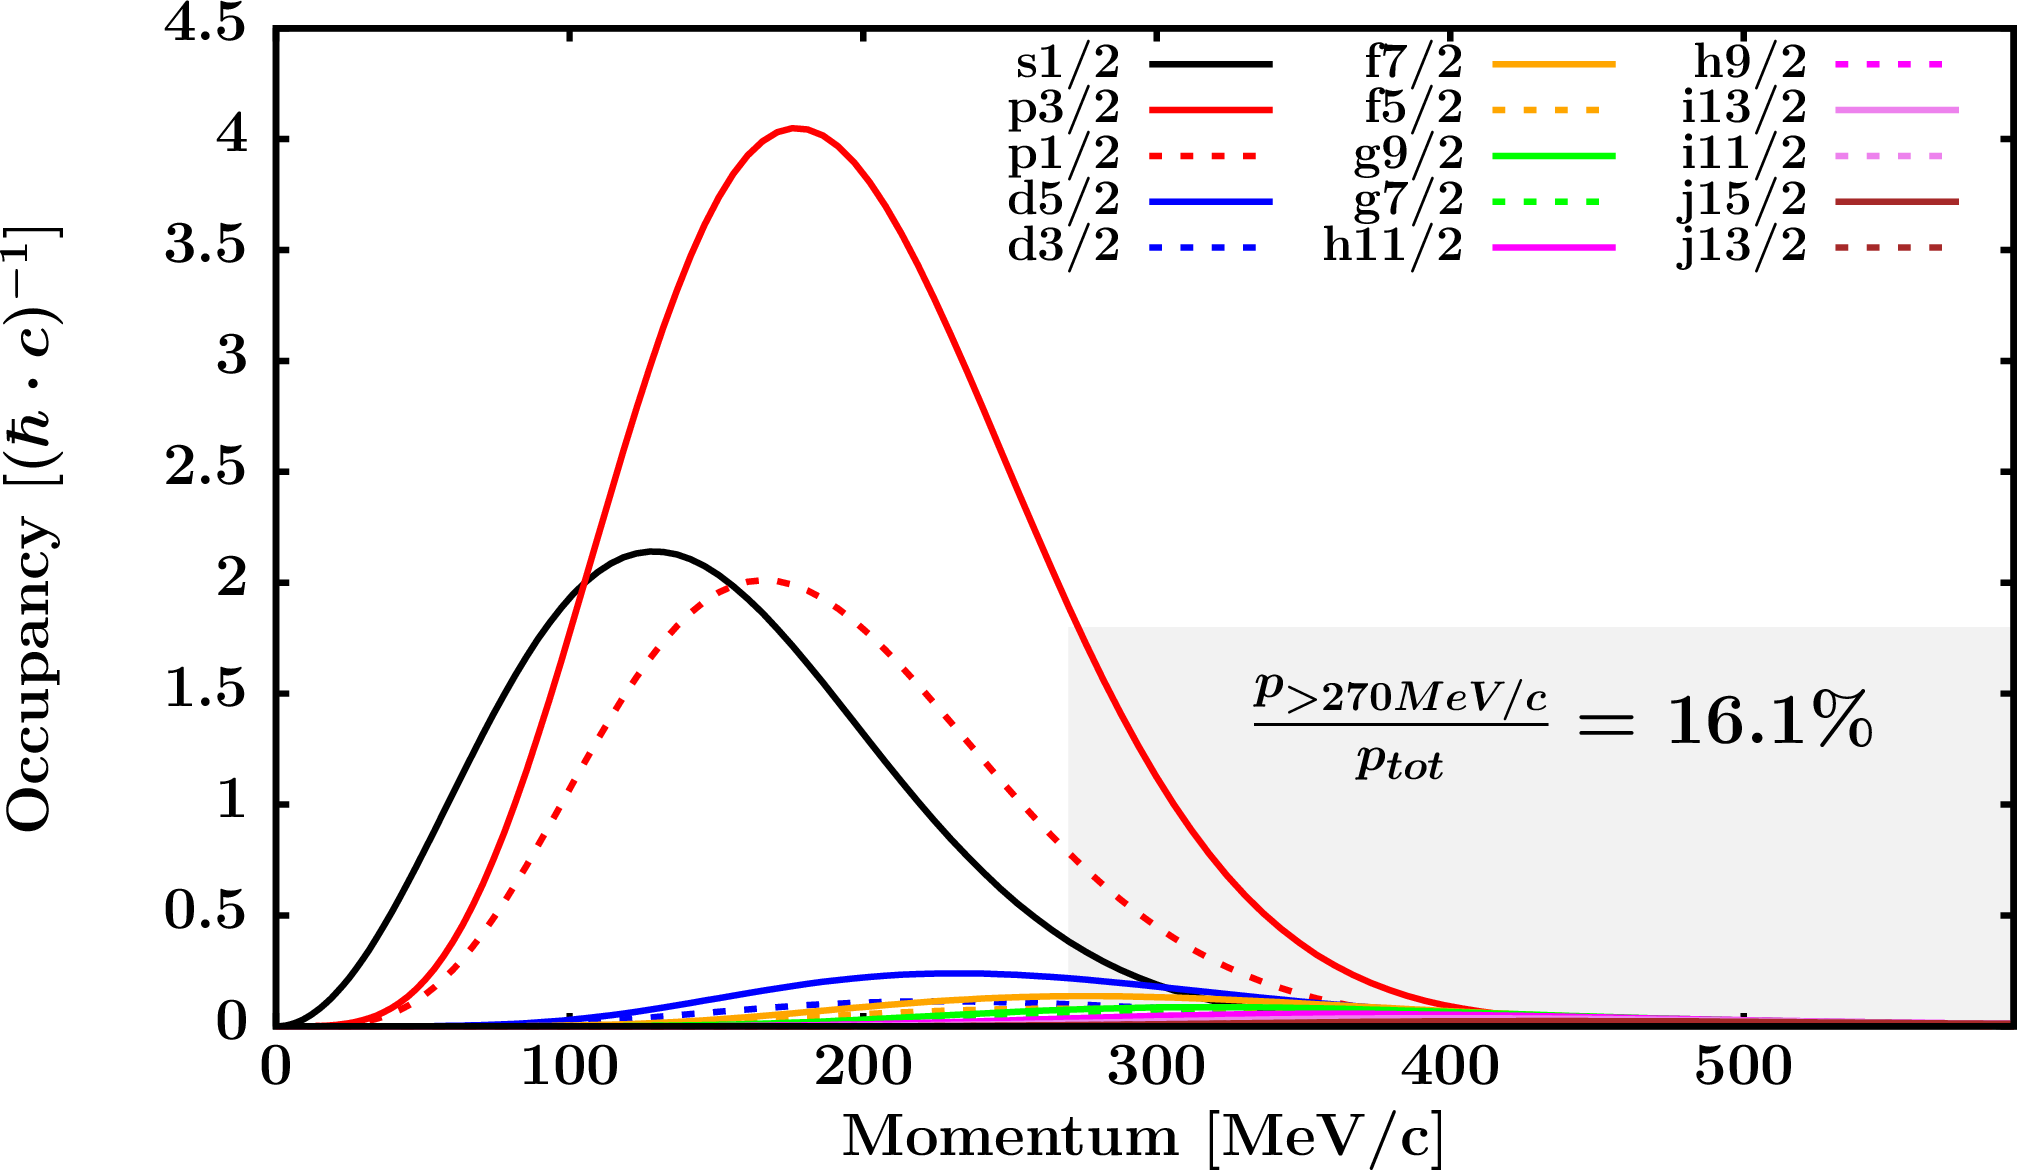
\includegraphics[width=\textwidth]{figures/o16_protonLJMomentumDistIntegral.png}
        \caption*{\oSix\ proton momentum distribution}
        \label{DOMFitData_o16_proton_momentumDist}
    \end{minipage}\hspace{6pt}
    \begin{minipage}{0.45\textwidth}
        \centering
        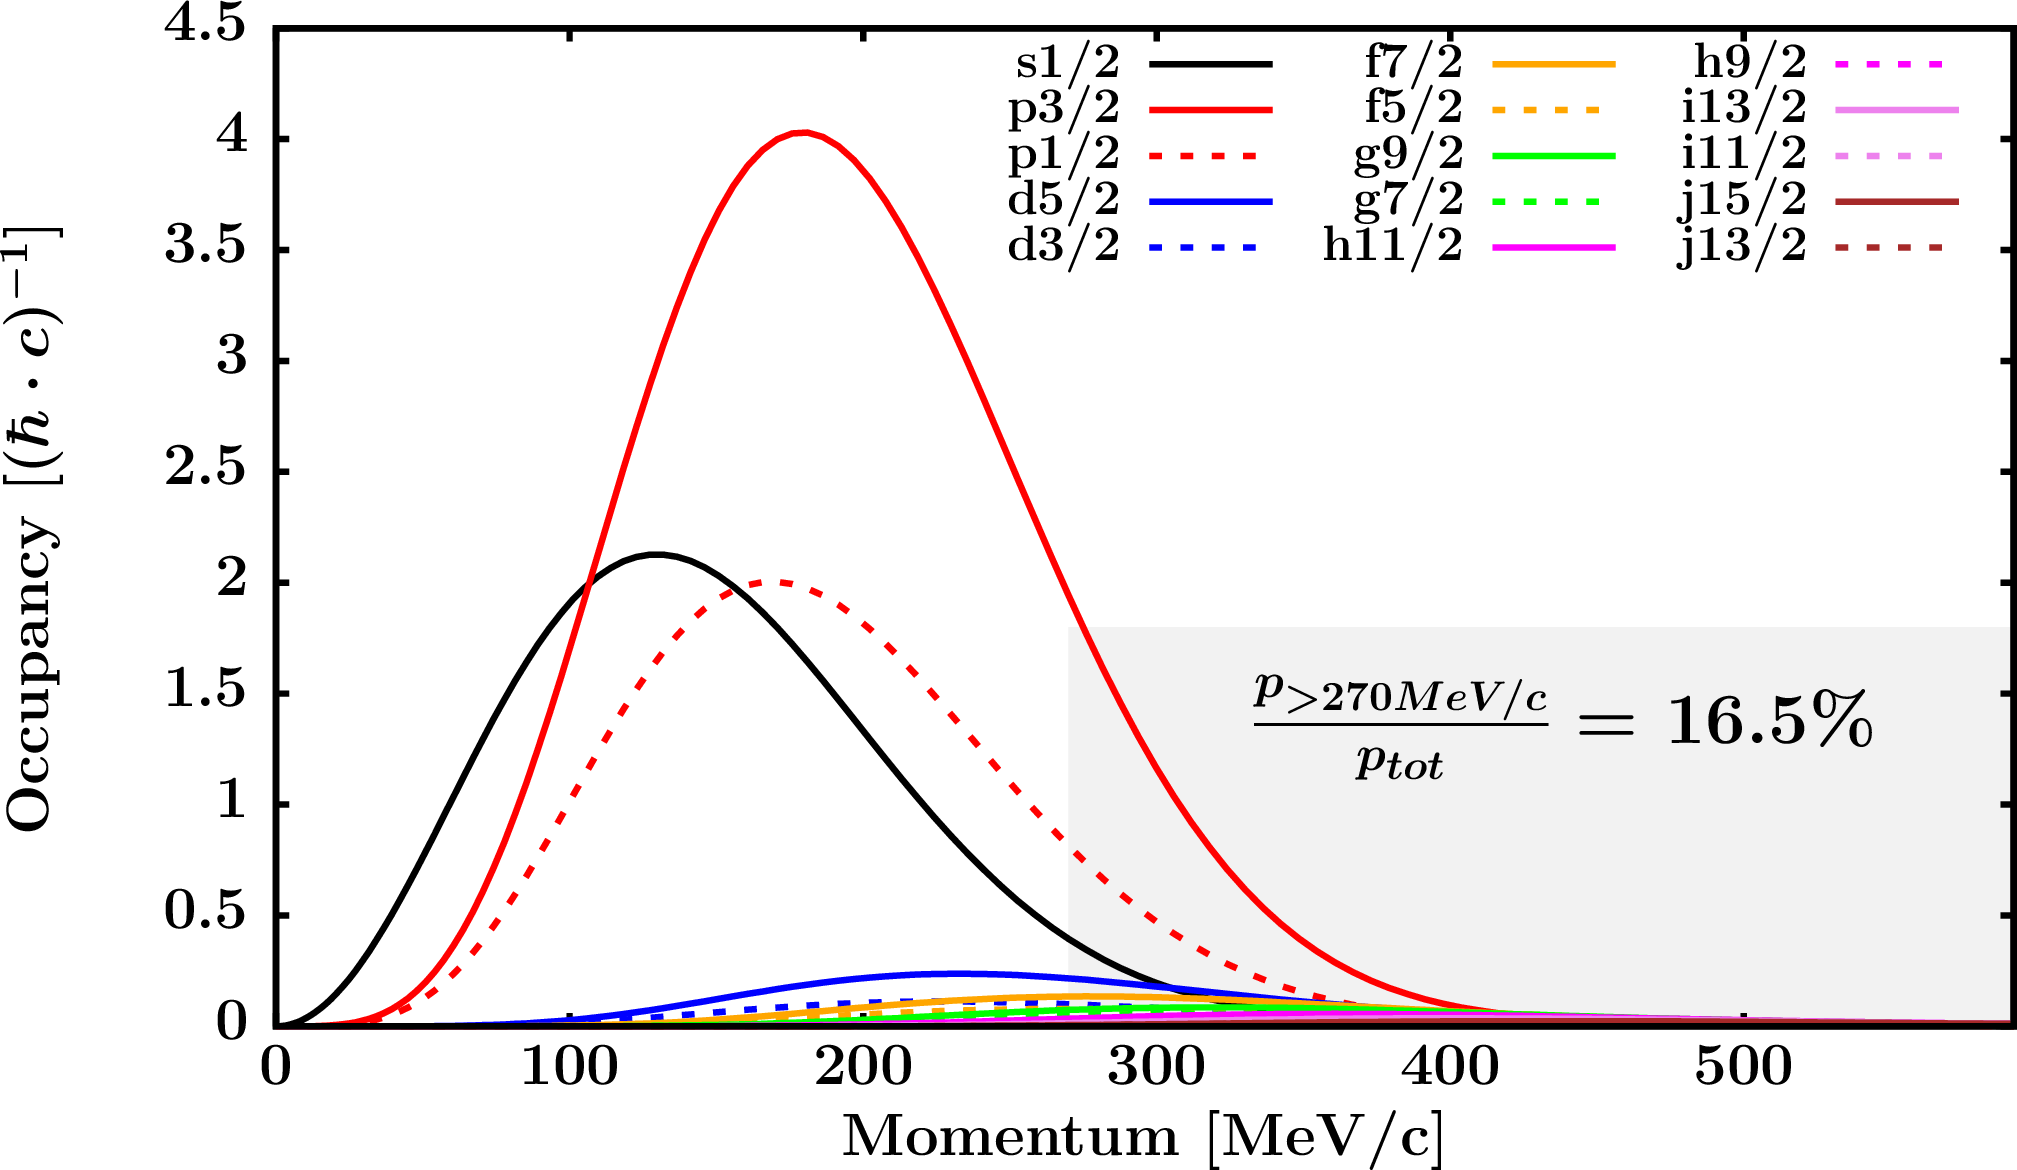
\includegraphics[width=\textwidth]{figures/o16_neutronLJMomentumDistIntegral.png}
        \caption*{\oSix\ neutron momentum distribution}
        \label{DOMFitData_o16_neutron_momentumDist}
    \end{minipage}
\end{figure}
\vspace{0.3in}
\begin{figure}[hbtp]
    \centering
    \begin{minipage}{0.45\textwidth}
        \centering
        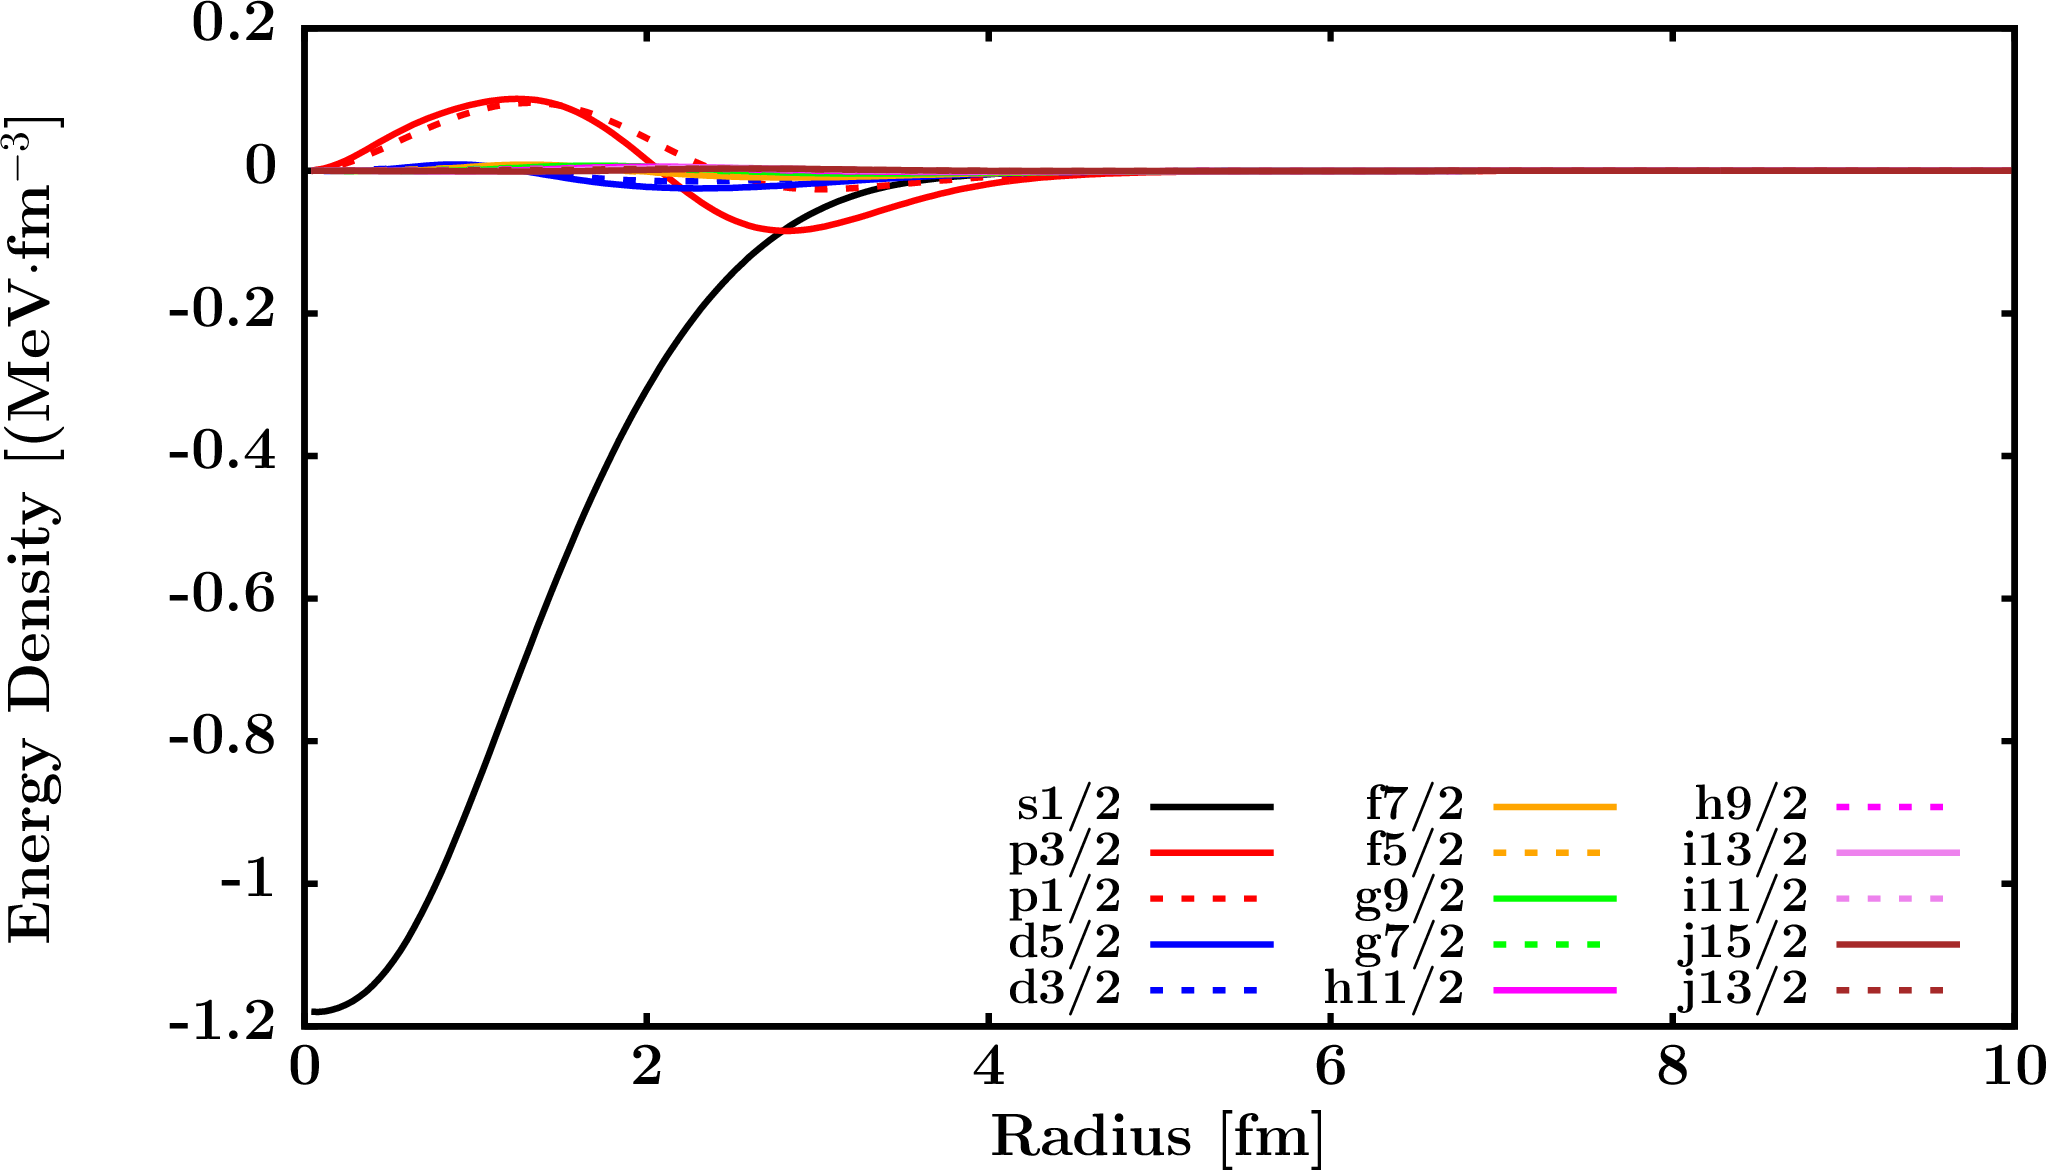
\includegraphics[width=\textwidth]{figures/o16_EnergyDist.png}
        \caption*{\oSix\ energy distribution by LJ}
        \label{DOMFitData_o16_proton_energyDistInt}
    \end{minipage}\hspace{6pt}
    \begin{minipage}{0.45\textwidth}
        \centering
        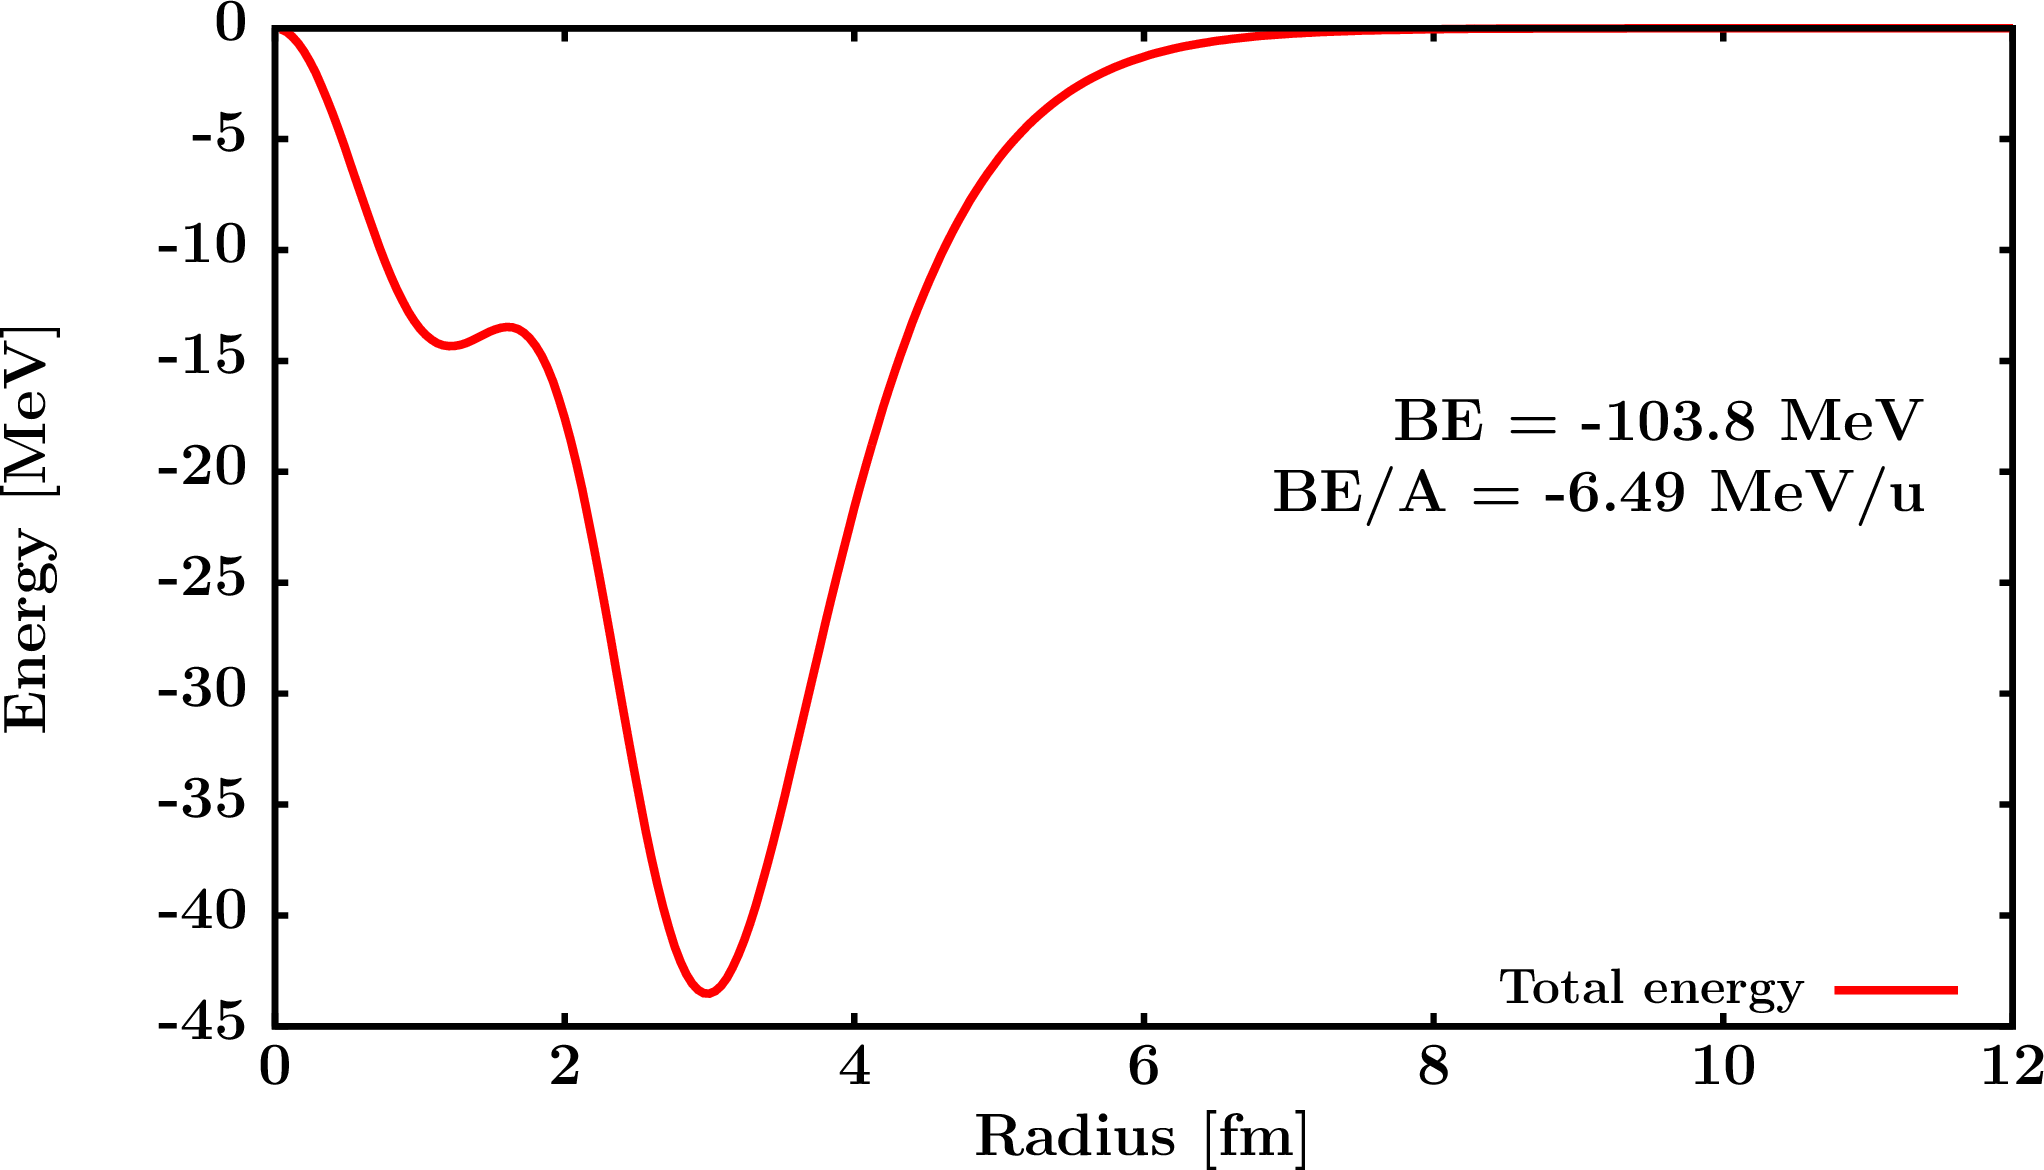
\includegraphics[width=\textwidth]{figures/o16_EnergyDistIntegral.png}
        \caption*{\oSix\ energy distribution integral}
        \label{DOMFitData_o16_neutron_energyDistInt}
    \end{minipage}
\end{figure}
\vspace{0.4in}
\begin{figure}[hbtp]
    \centering
    \begin{minipage}{0.70\textwidth}
        \centering
        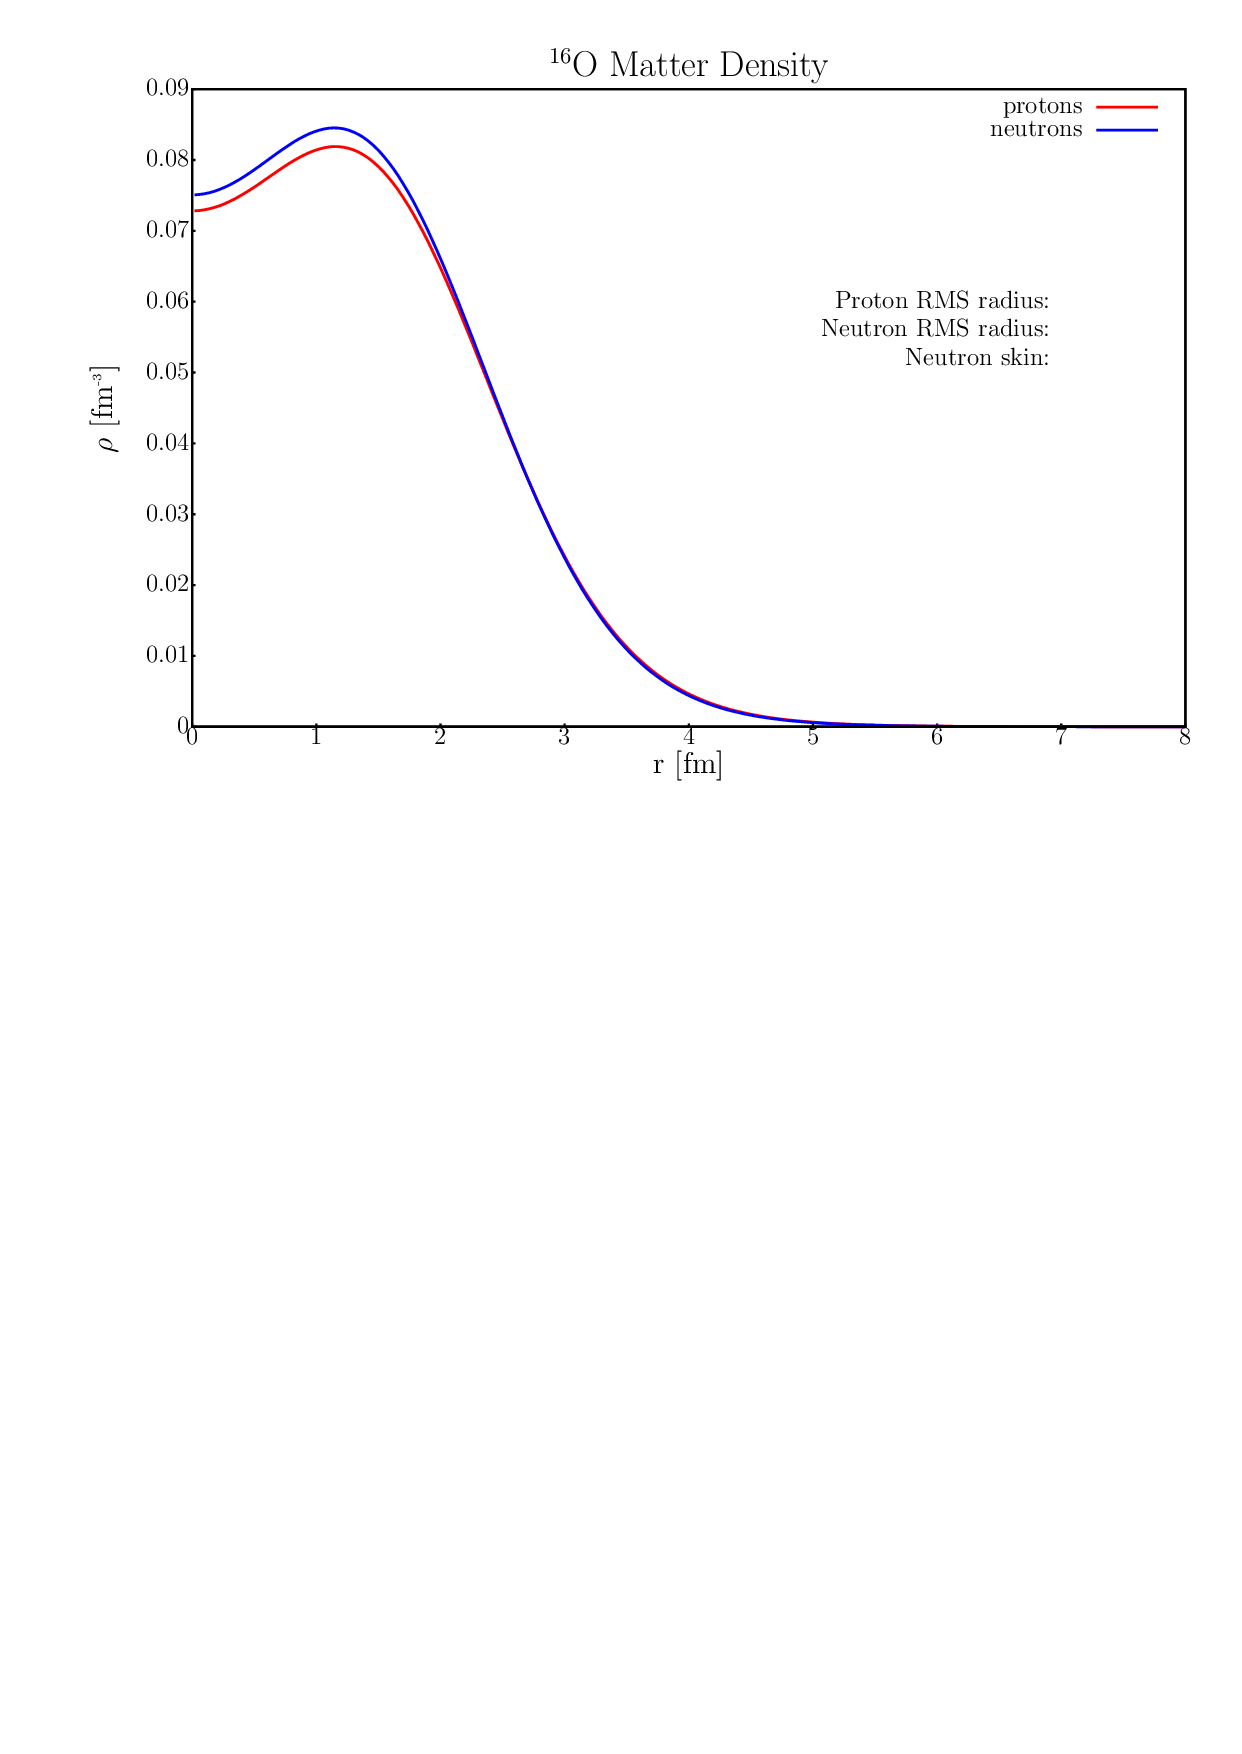
\includegraphics[width=\linewidth]{figures/o16_matterDensity.png}
        \caption*{\oSix\ matter density distribution}
        \label{DOMFitData_o16_matterDensity}
    \end{minipage}
\end{figure}

\section{DOM fit of \oEight}
\label{o18DOMOutput}
\begin{figure}[hbtp]
    \centering
    \begin{minipage}{0.47\textwidth}
        \centering
        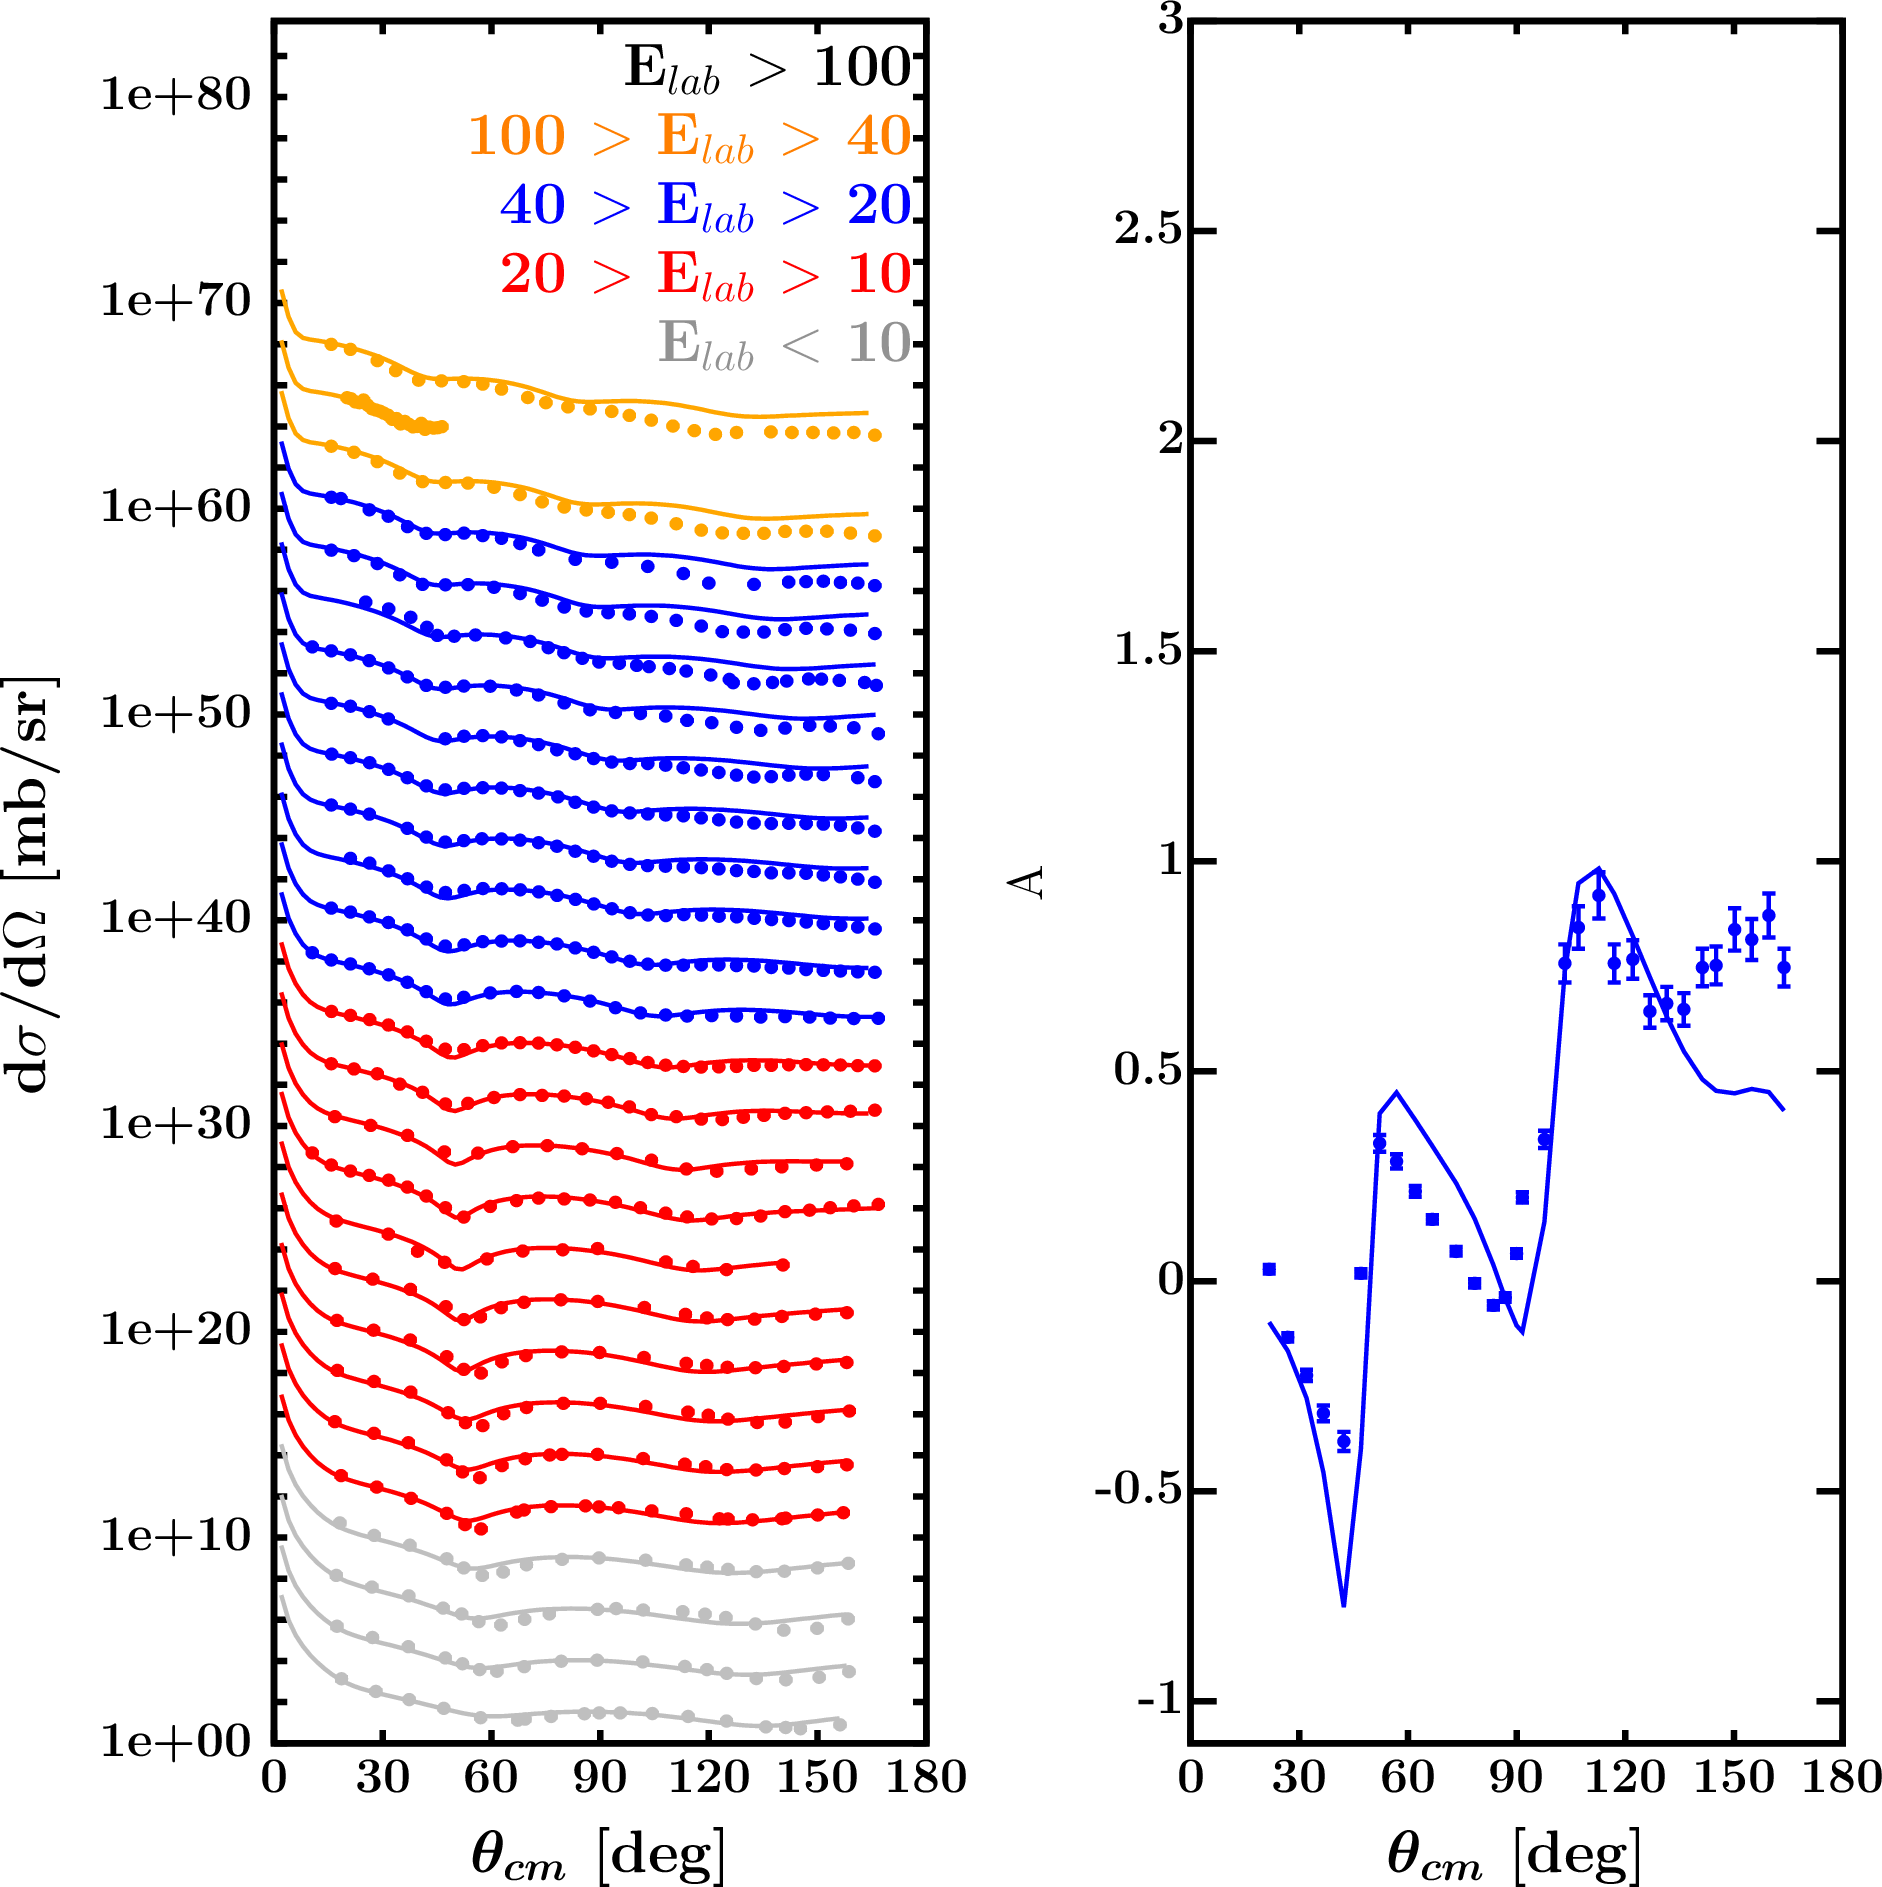
\includegraphics[width=\textwidth]{figures/o18_protonElastic.png}
        \caption*{\oEight\ proton elastic scattering}
        \label{DOMFitData_o18_proton_elastic}
    \end{minipage}\hspace{6pt}
    \begin{minipage}{0.47\textwidth}
        \centering
        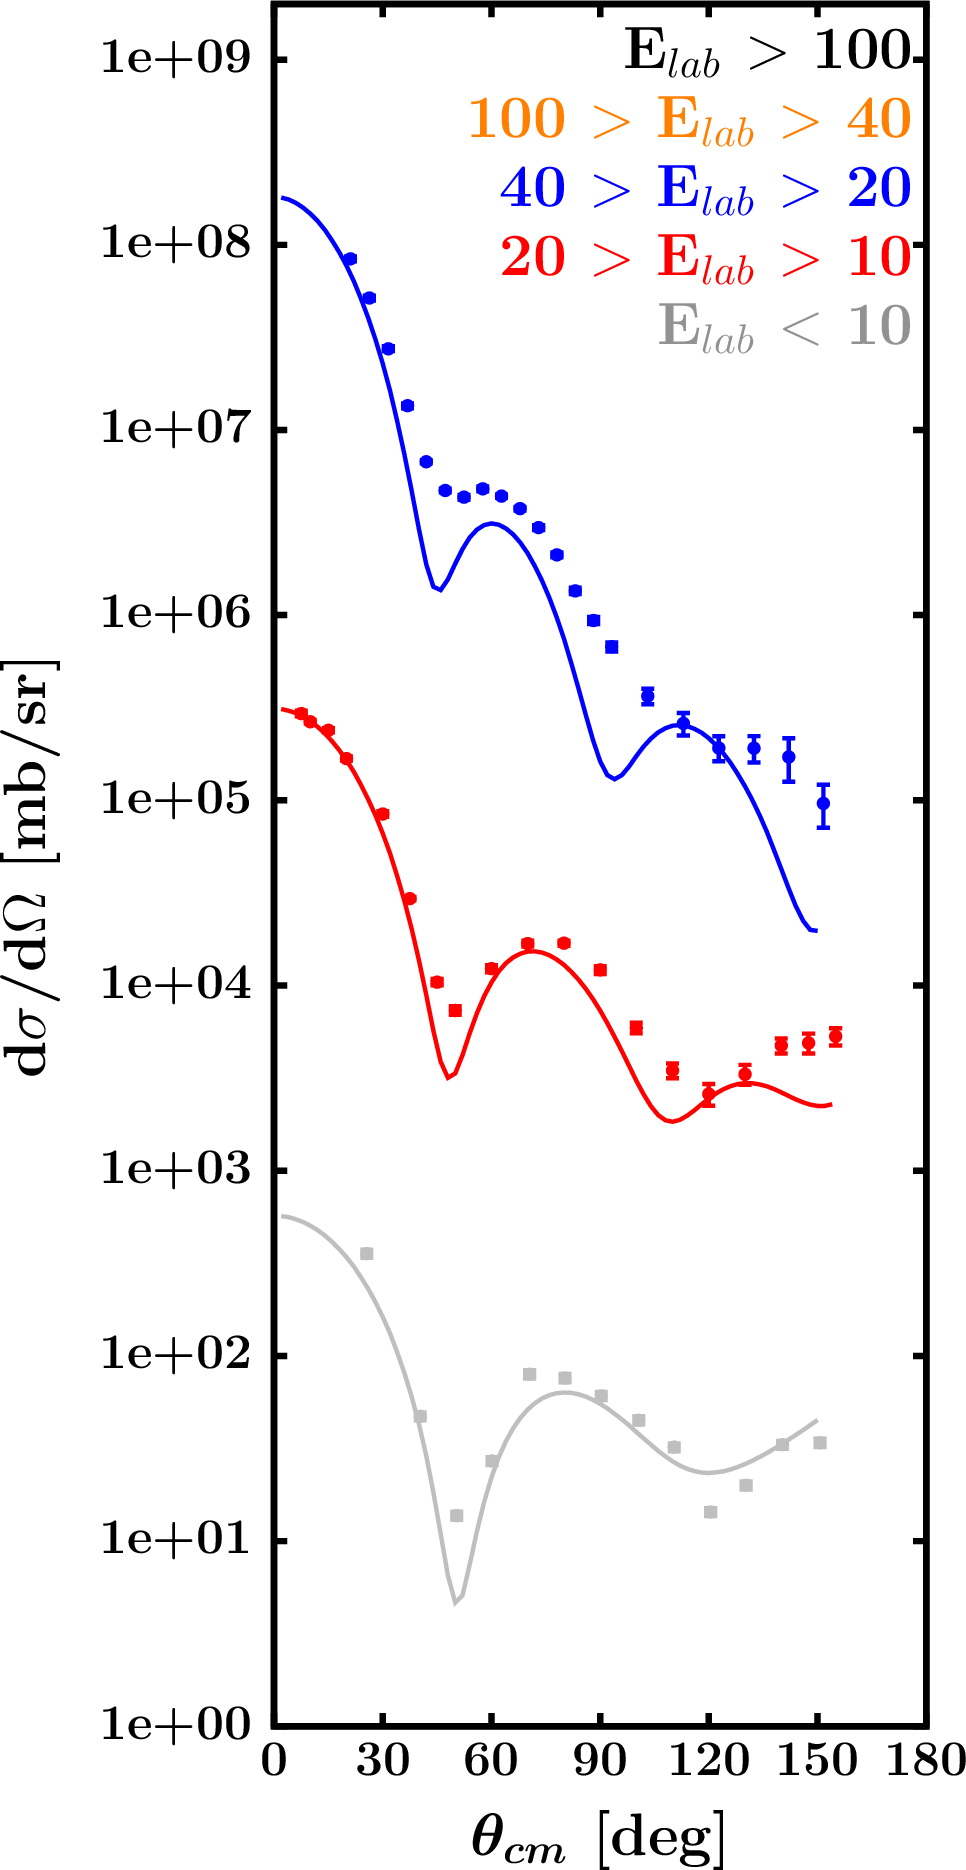
\includegraphics[width=0.52\textwidth]{figures/o18_neutronElastic.png}
        \caption*{\oEight\ neutron elastic scattering}
        \label{DOMFitData_o18_neutron_elastic}
    \end{minipage}
\end{figure}
\vspace{0.70in}
\begin{figure}[hbtp]
    \centering
    \begin{minipage}{0.47\textwidth}
        \centering
        %
\includegraphics[width=\linewidth]{figures/o18_protonInelastic.png}
        No \oEight\ proton \rxn\\ data were available
        \label{DOMFitData_o18_proton_inelastic}
    \end{minipage}\hspace{6pt}
    \begin{minipage}{0.47\textwidth}
        \centering
        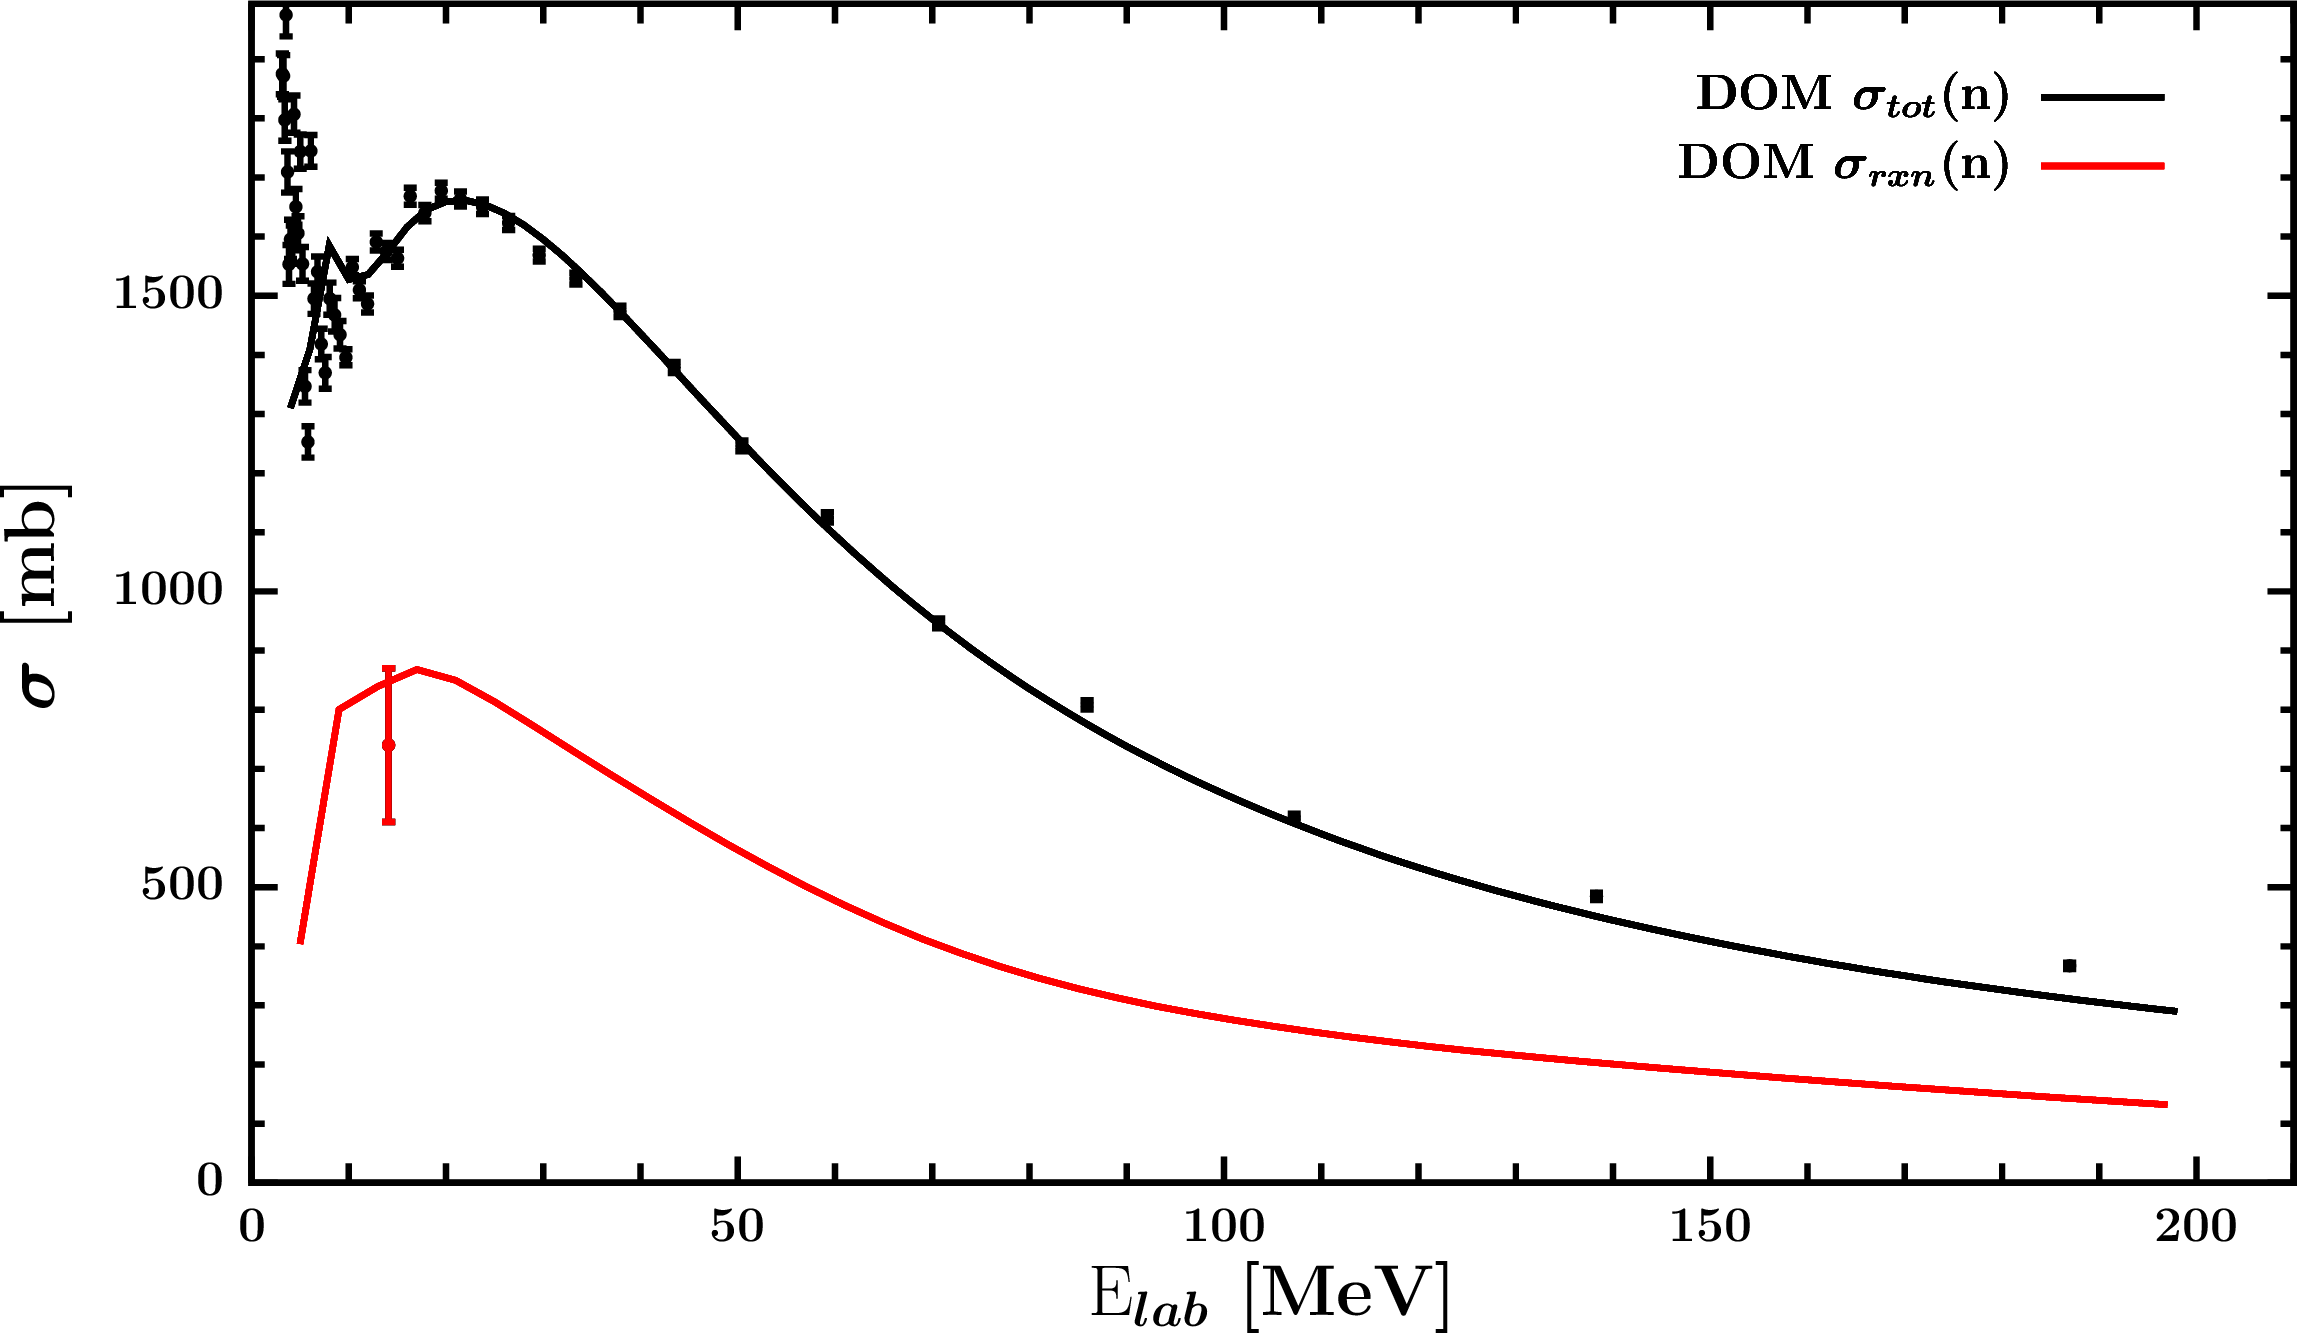
\includegraphics[width=\textwidth]{figures/o18_neutronInelastic.png}
        \caption*{\oEight\ neutron \rxn\ and \tot}
        \label{DOMFitData_o18_neutron_inelastic}
    \end{minipage}
\end{figure}
%\afterpage{\clearpage}
\begin{figure}[hbtp]
    \centering
    \begin{minipage}{0.42\textwidth}
        \centering
        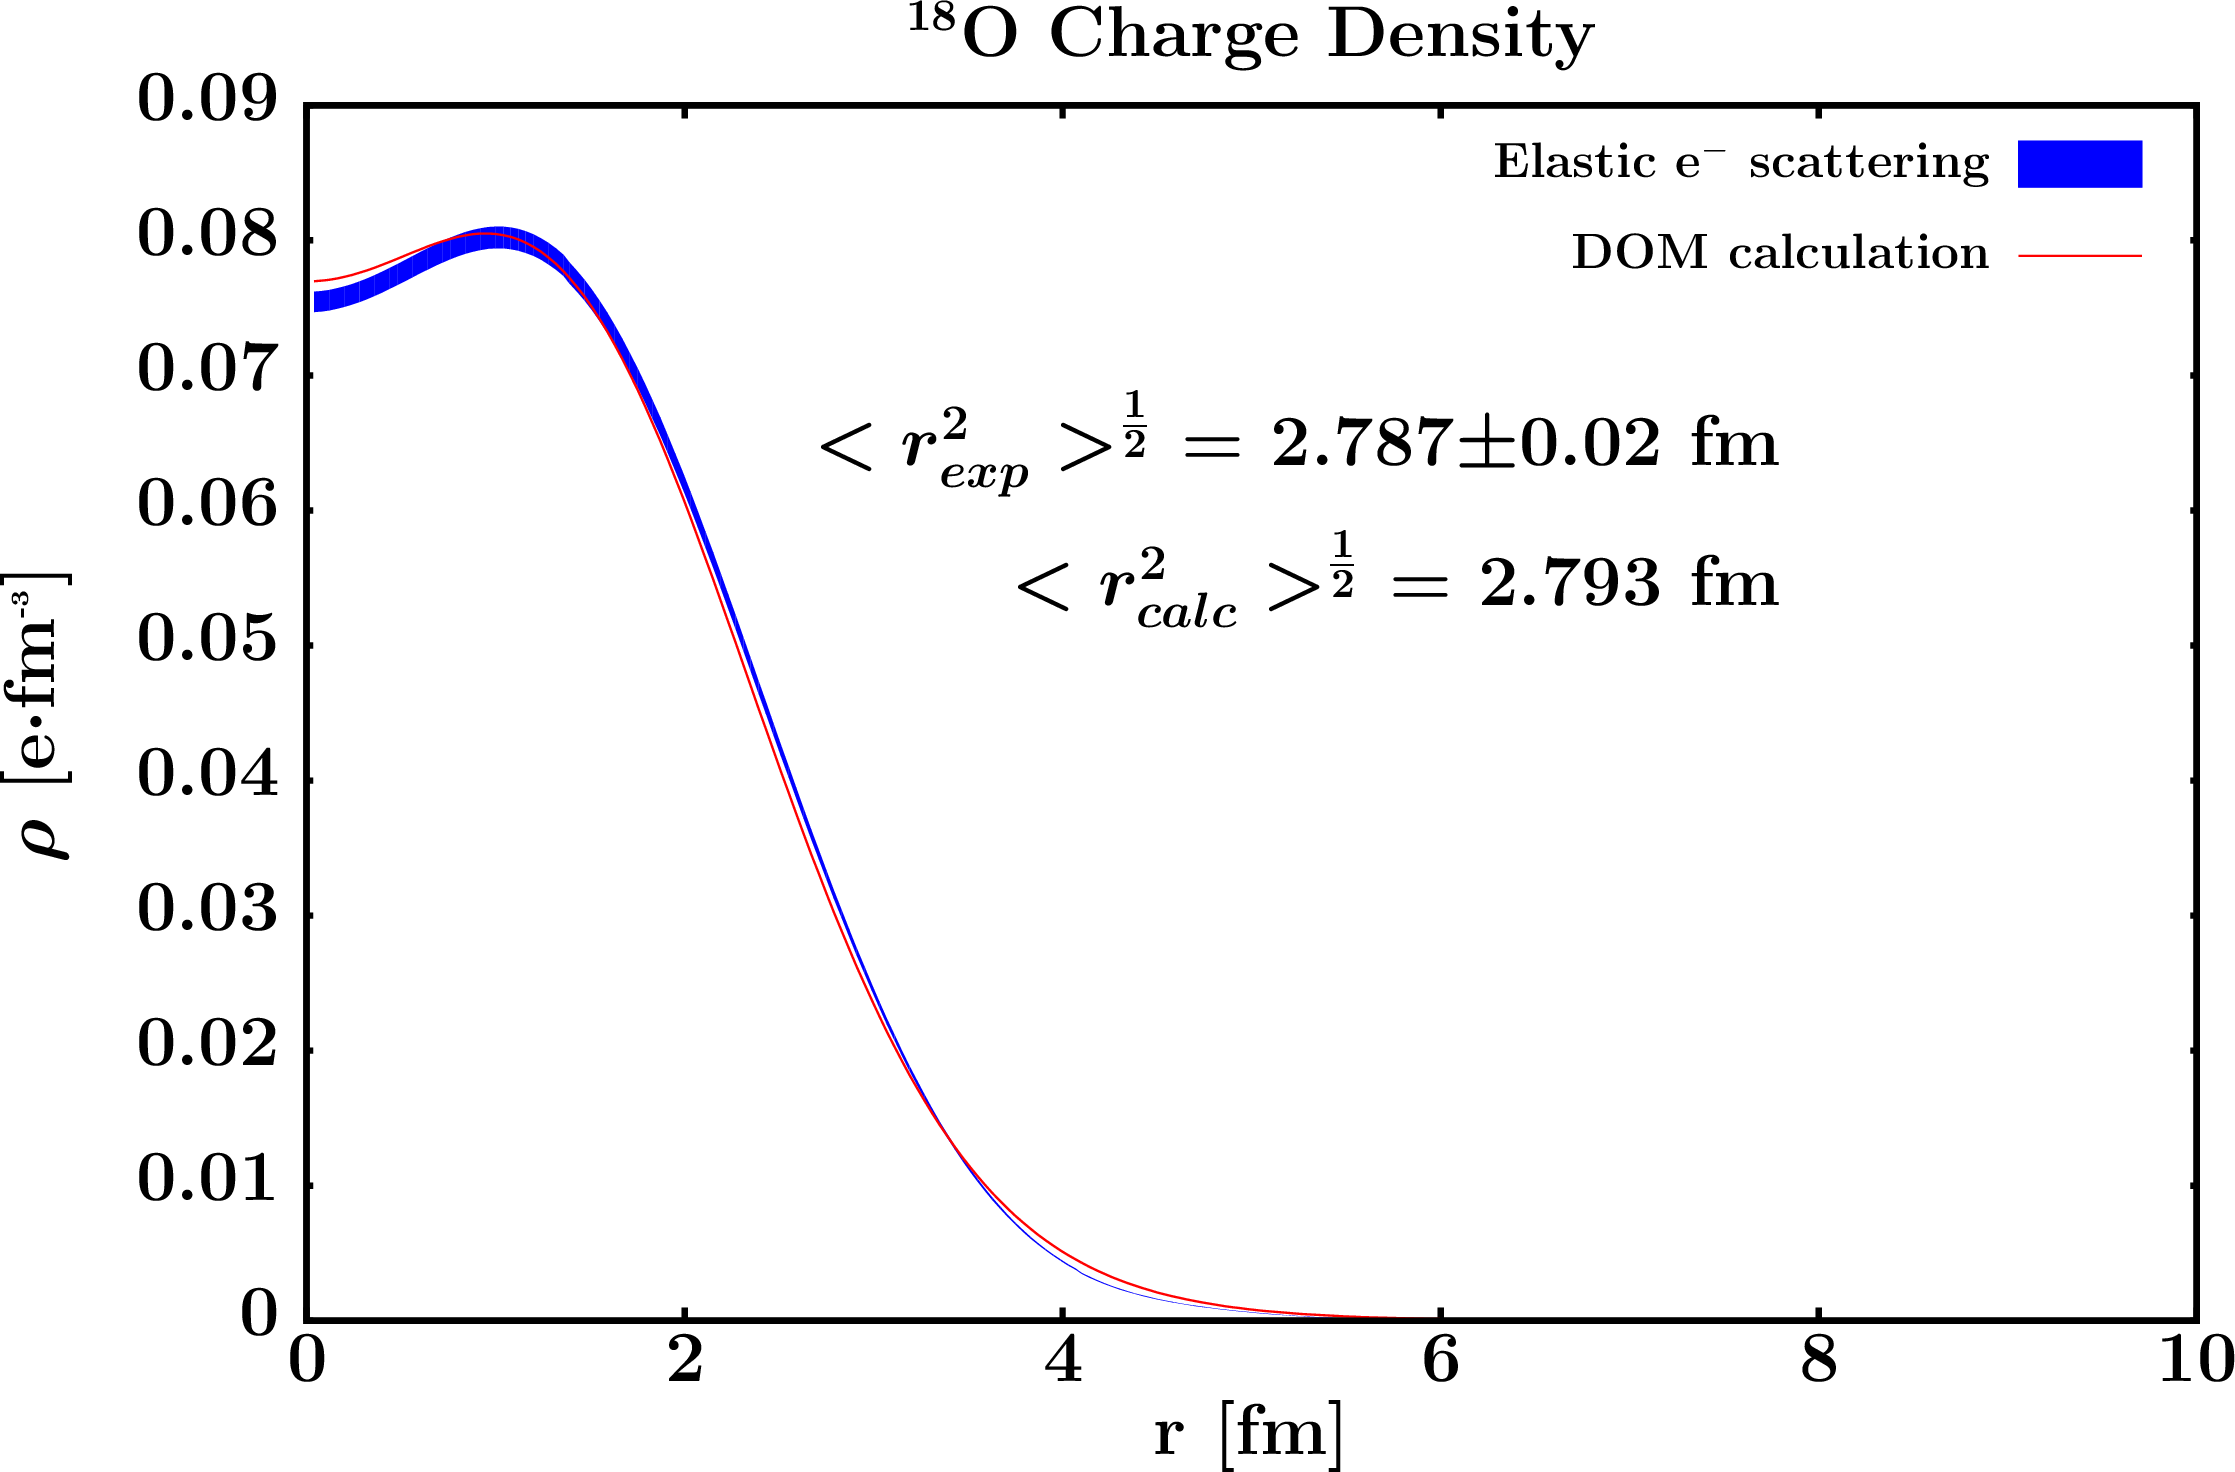
\includegraphics[width=\textwidth]{figures/o18_chargeDensity.png}
        \caption*{\oEight\ charge density}
        \label{DOMFitData_o18_chargeDensity}
    \end{minipage}\hspace{6pt}
    \begin{minipage}{0.42\textwidth}
        \centering
        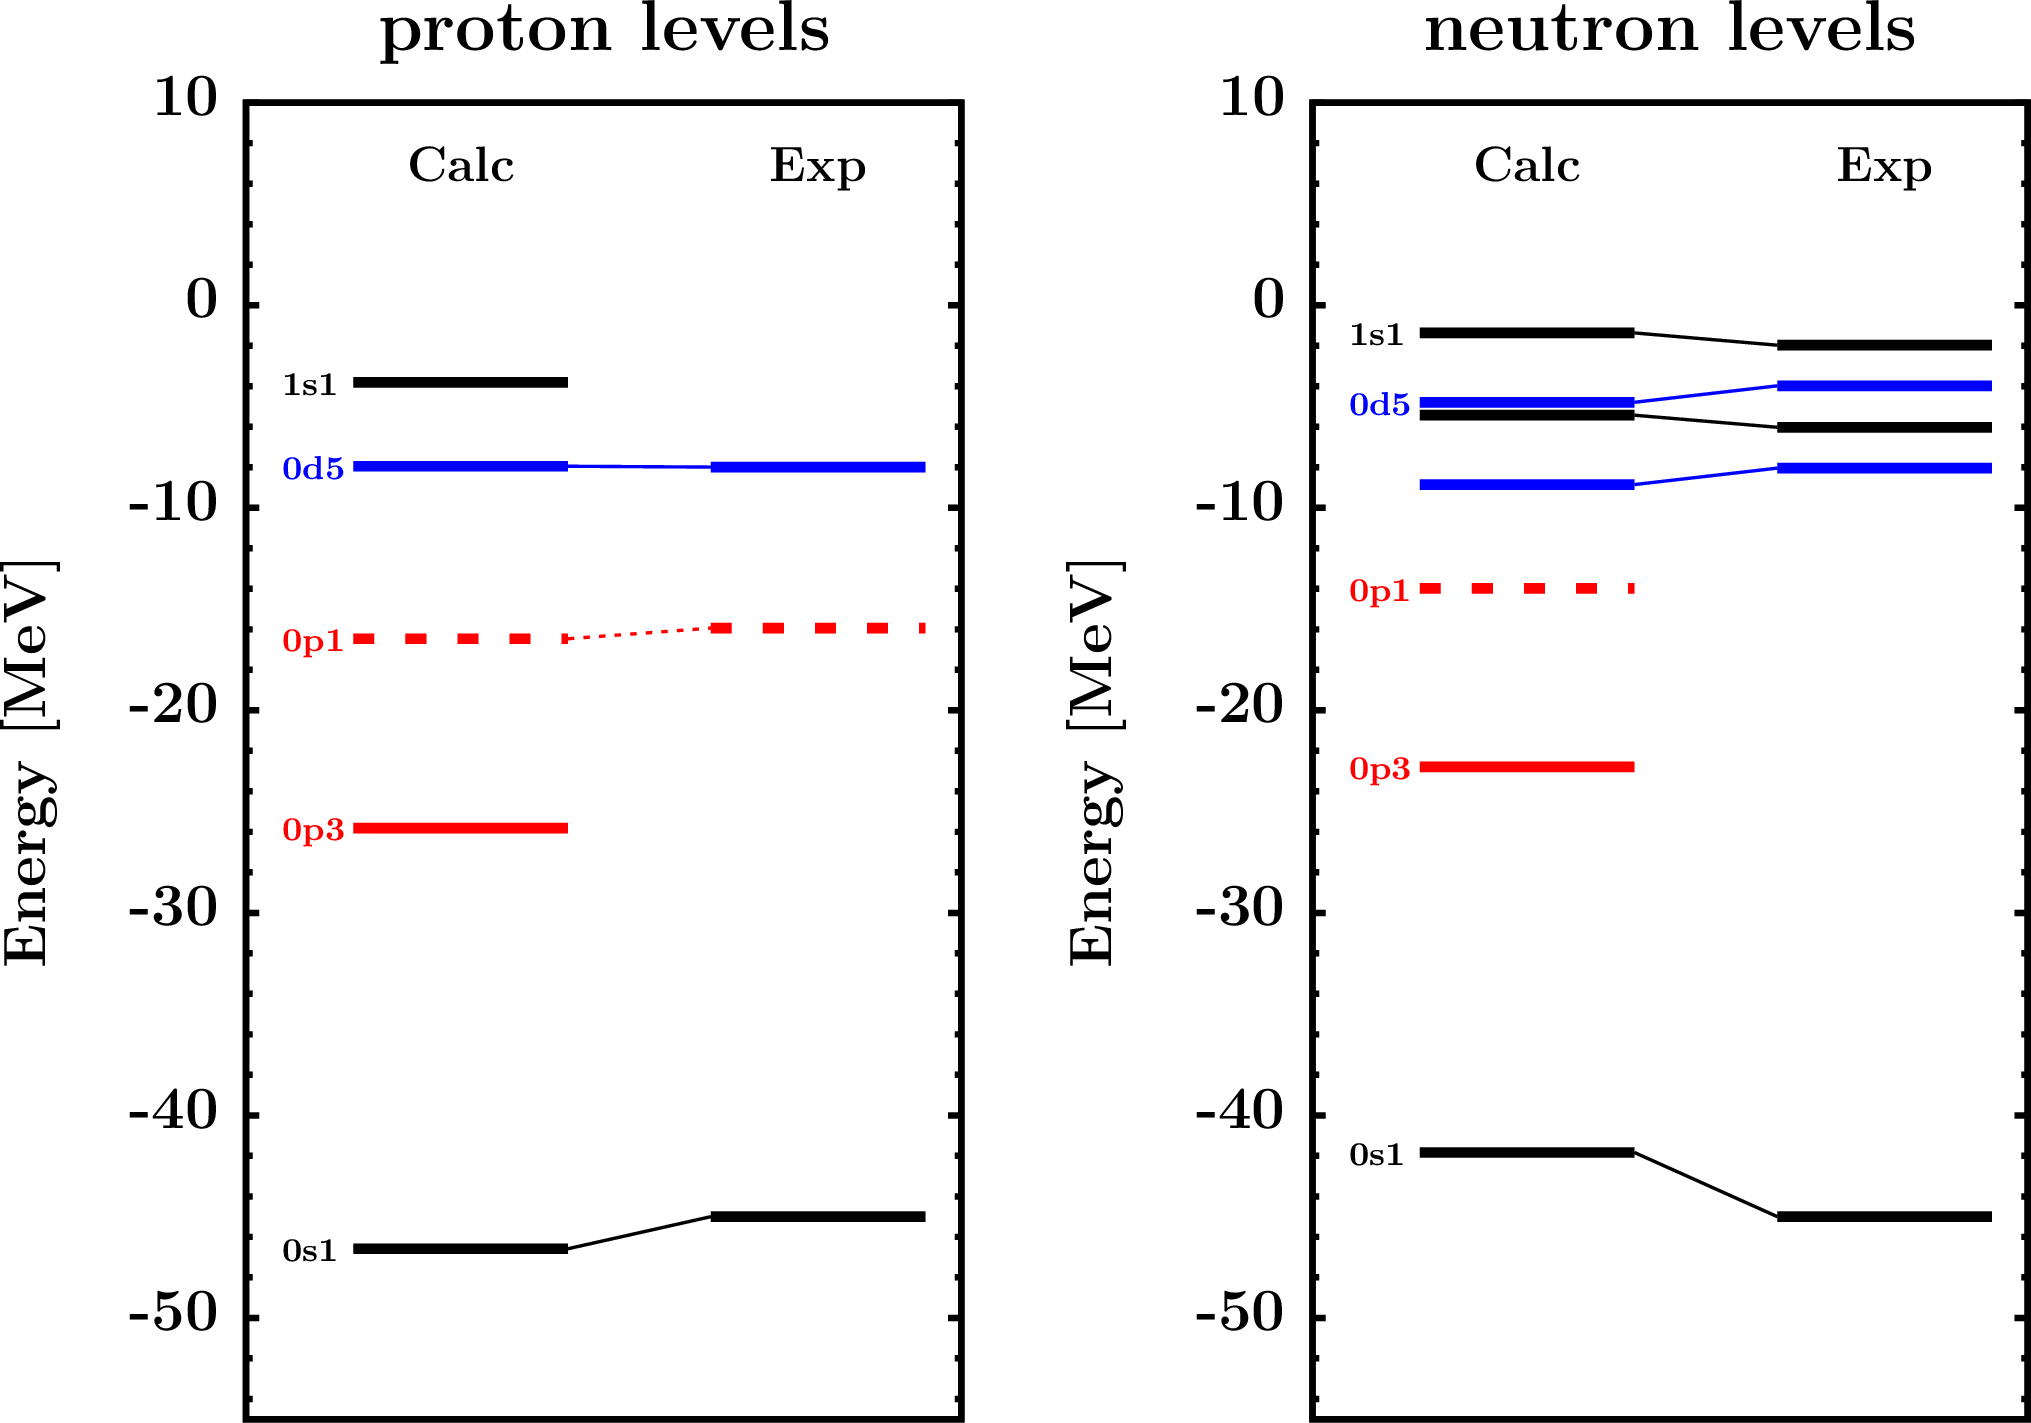
\includegraphics[width=\textwidth]{figures/o18_SPLevels.png}
        \caption*{\oEight\ single-particle levels}
        \label{DOMFitData_o18_SPLevels}
    \end{minipage}
\end{figure}
%\vspace{0.3in}
\begin{figure}[hbtp]
    \centering
    \begin{minipage}{0.42\textwidth}
        \centering
        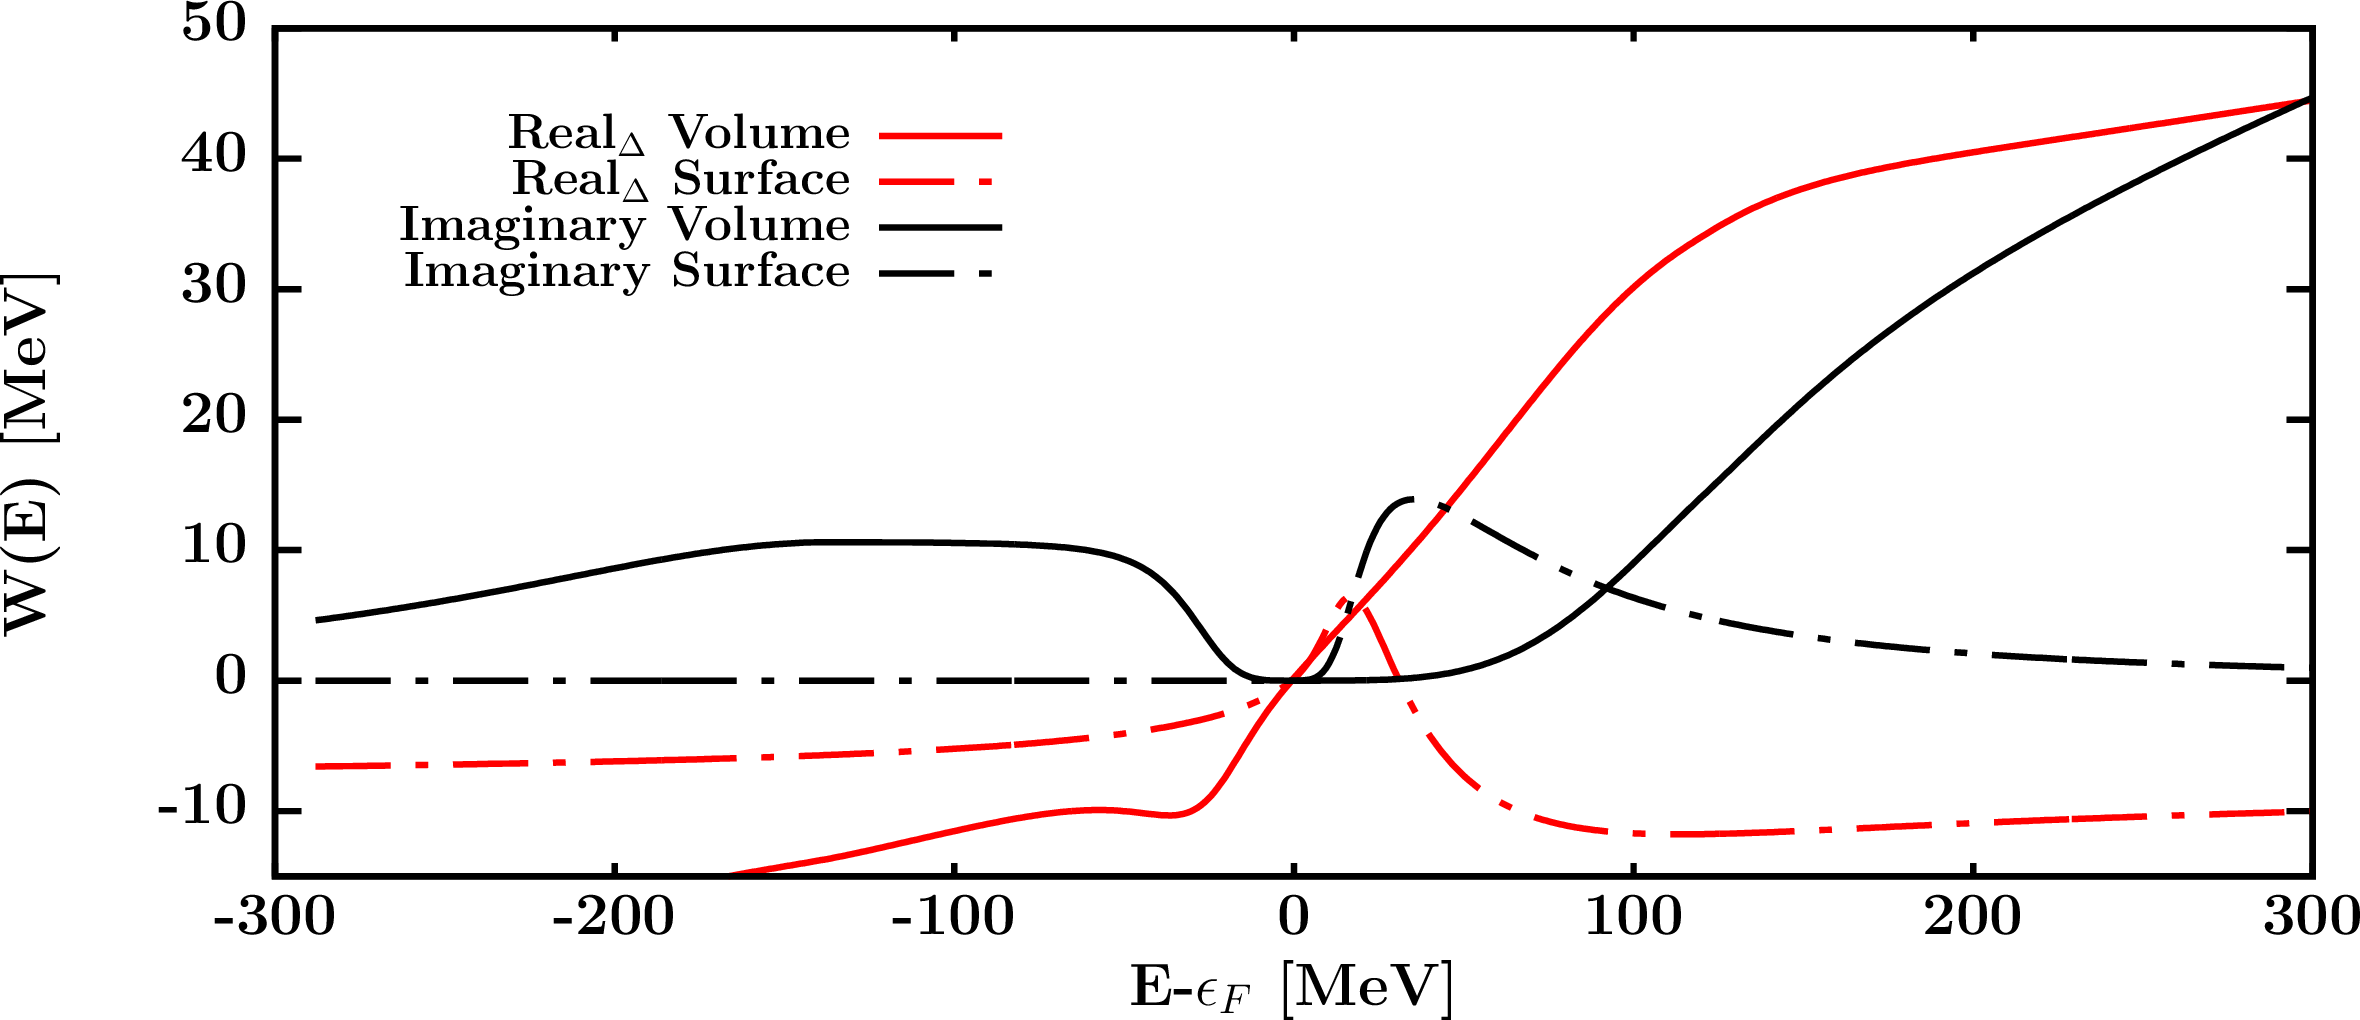
\includegraphics[width=\textwidth]{figures/o18_protonPotentials.png}
        \caption*{\footnotesize\oEight\ proton potential energy dependence}
        \label{DOMFitData_o18_proton_potentialComponent_energy}
    \end{minipage}\hspace{6pt}
    \begin{minipage}{0.42\textwidth}
        \centering
        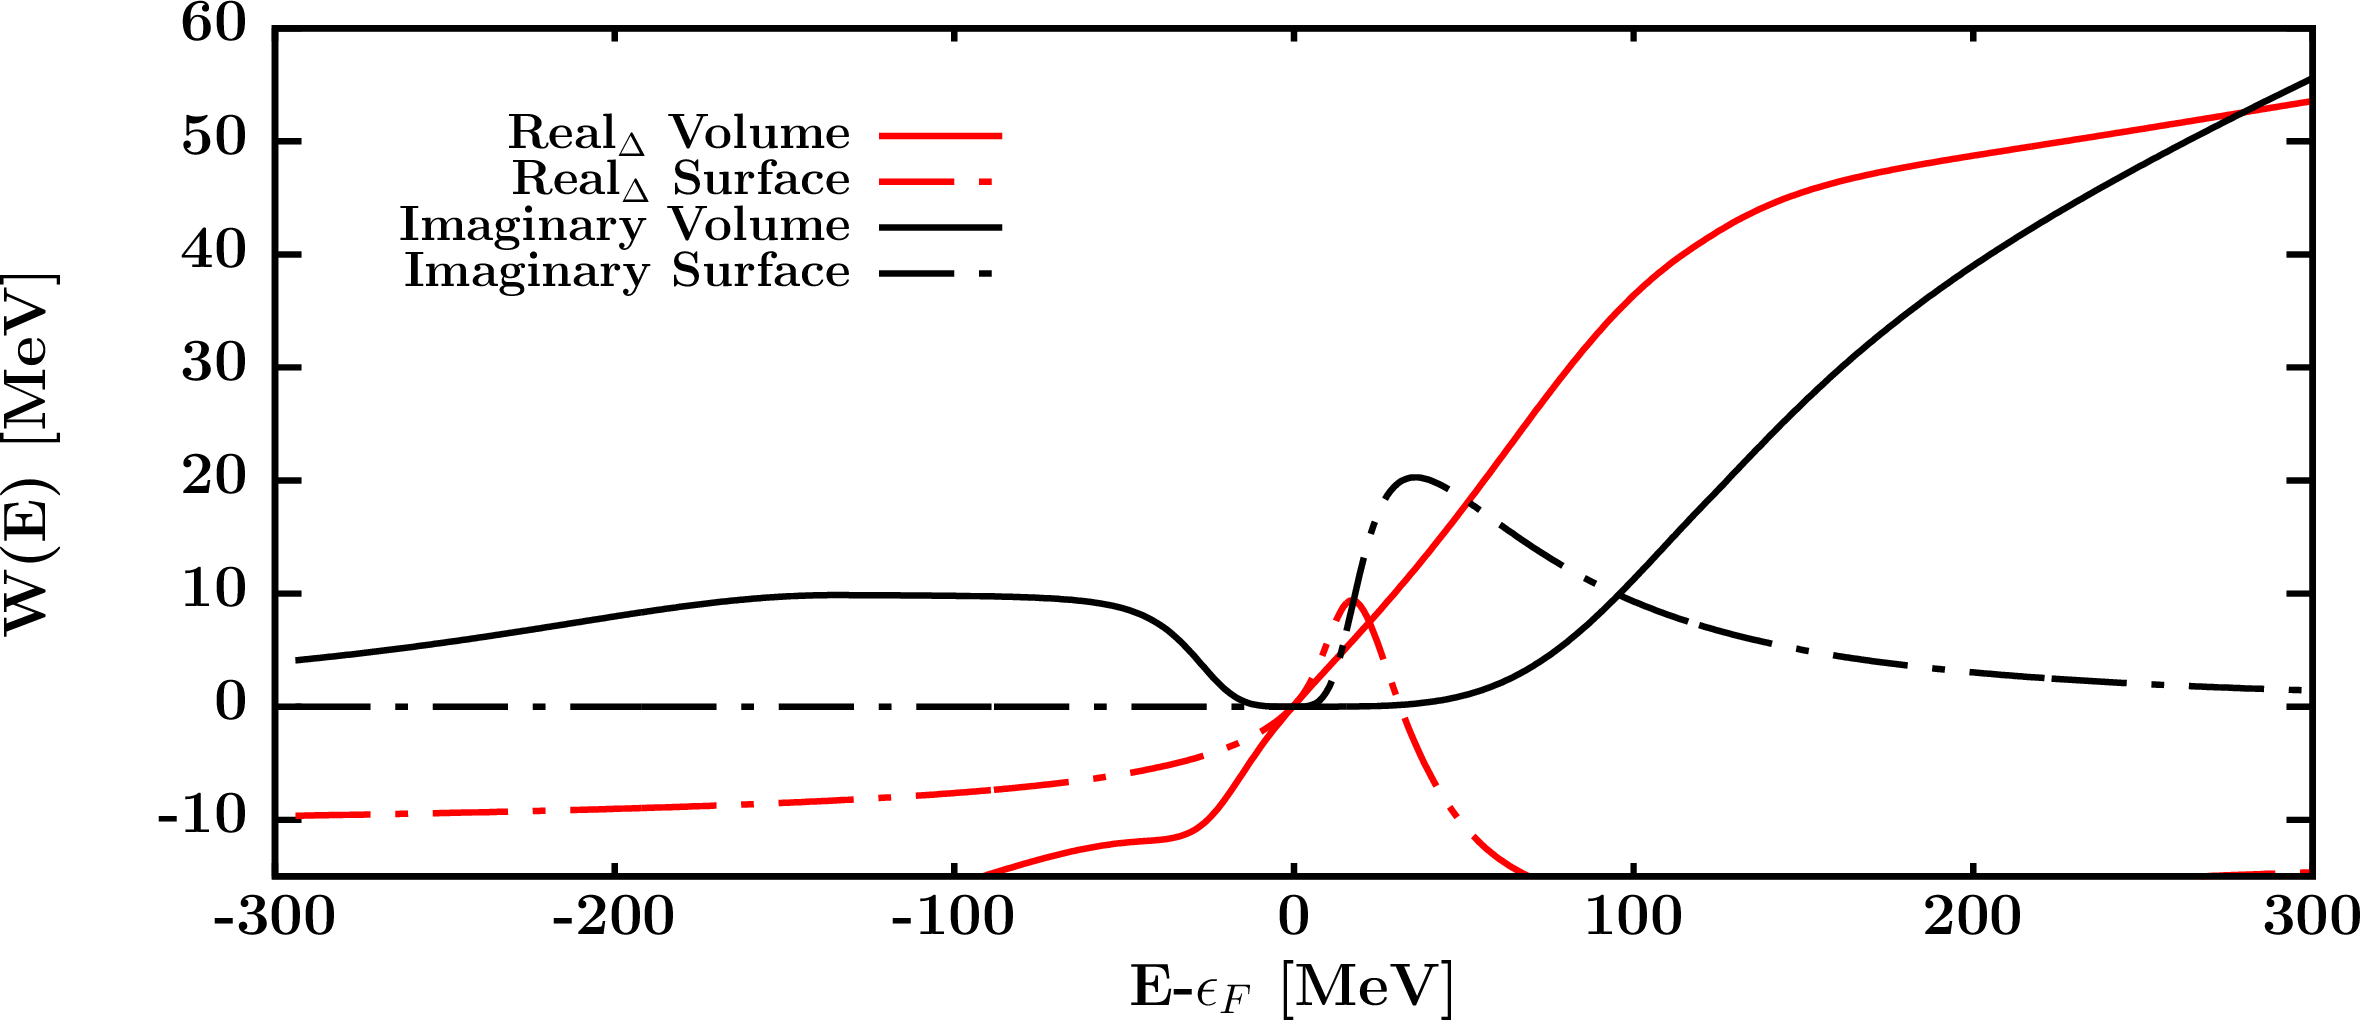
\includegraphics[width=\textwidth]{figures/o18_neutronPotentials.png}
        \caption*{\footnotesize\oEight\ neutron potential energy dependence}
        \label{DOMFitData_o18_neutron_potentialComponent_energy}
    \end{minipage}
\end{figure}
%\vspace{0.3in}
\begin{figure}[hbtp]
    \centering
    \begin{minipage}{0.42\textwidth}
        \centering
        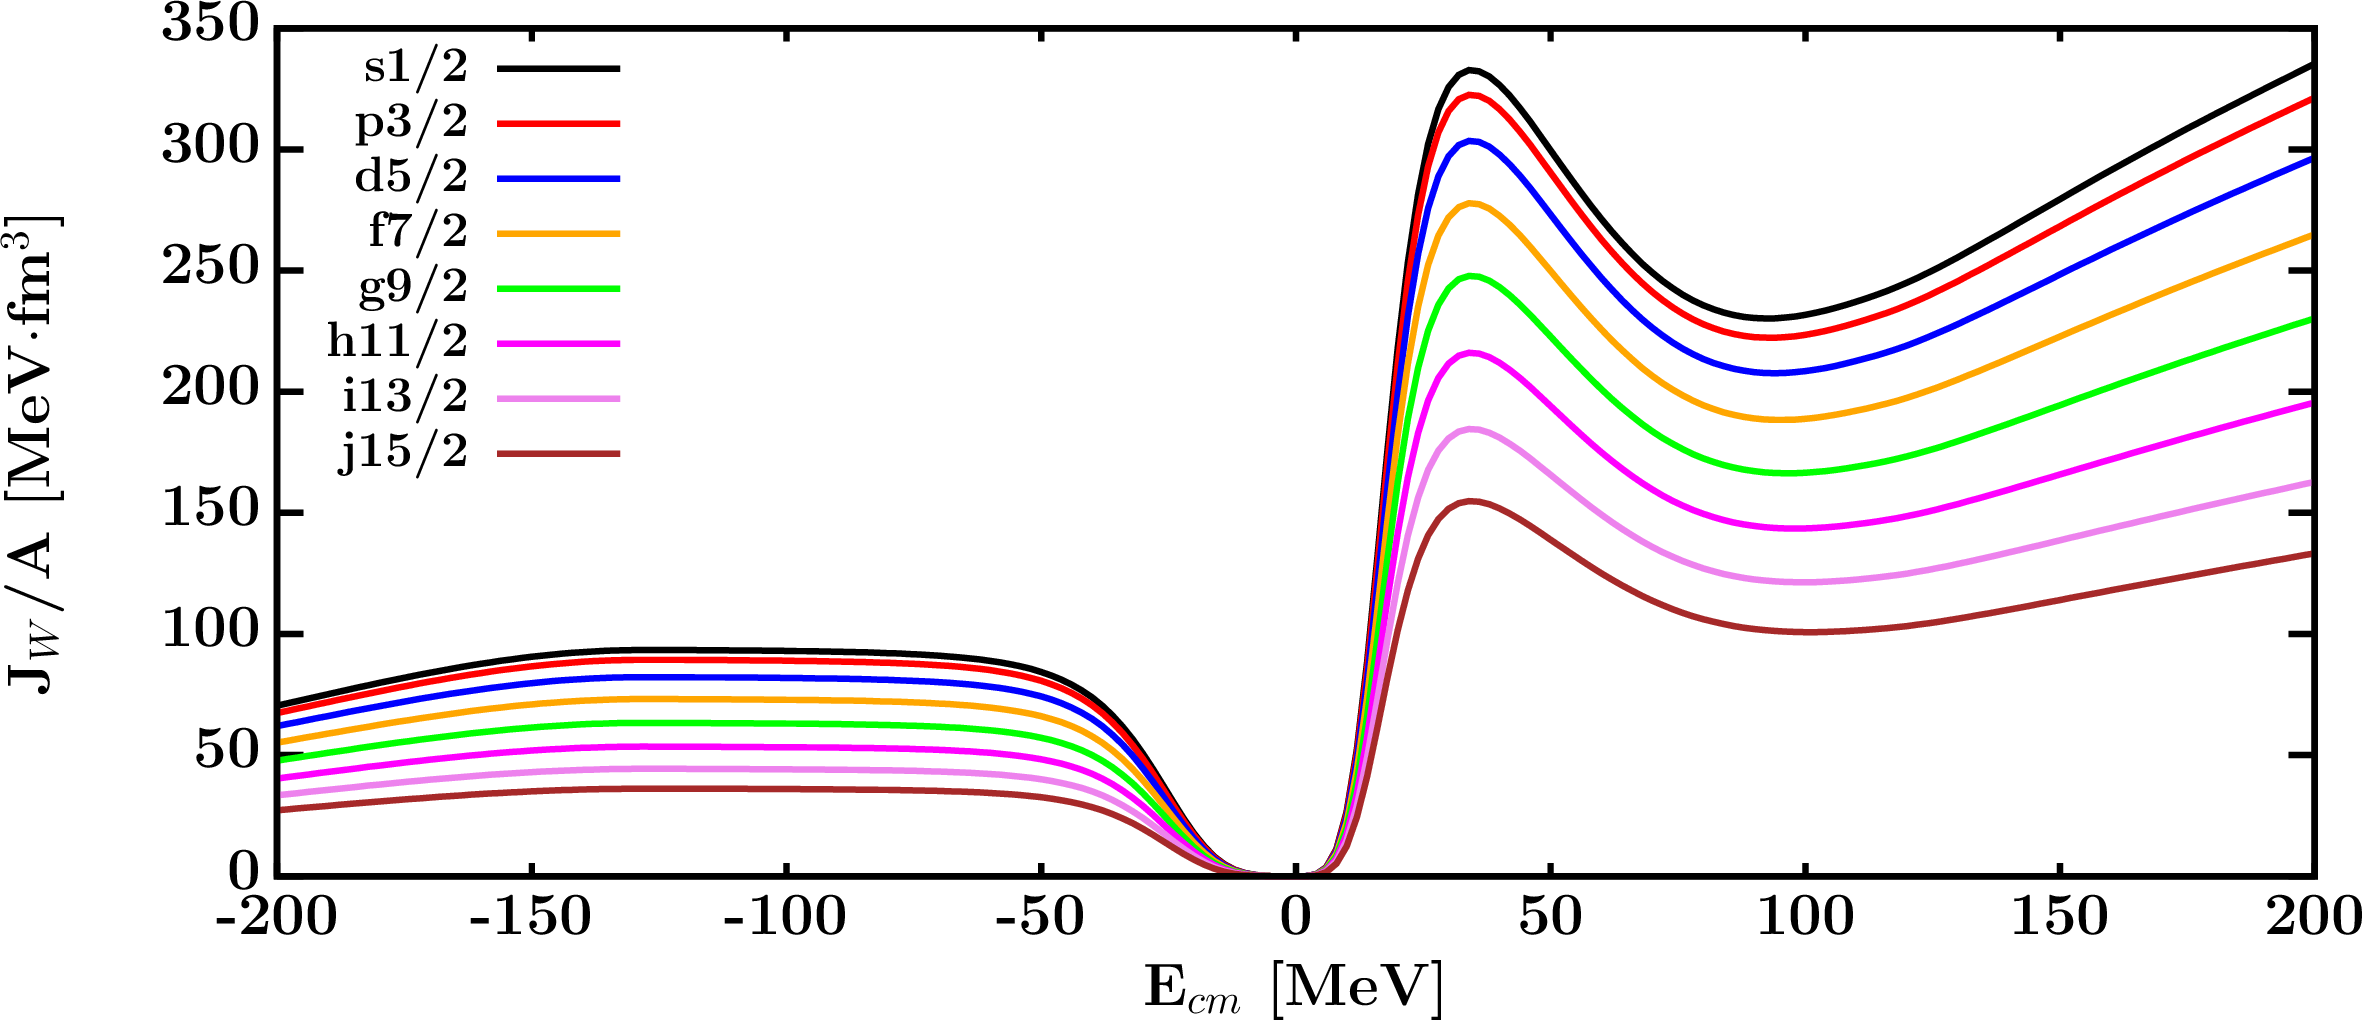
\includegraphics[width=\textwidth]{figures/o18_protonVolumeIntegrals.png}
        \caption*{\oEight\ proton volume integral}
        \label{DOMFitData_o18_proton_potentialIntegral}
    \end{minipage}\hspace{6pt}
    \begin{minipage}{0.42\textwidth}
        \centering
        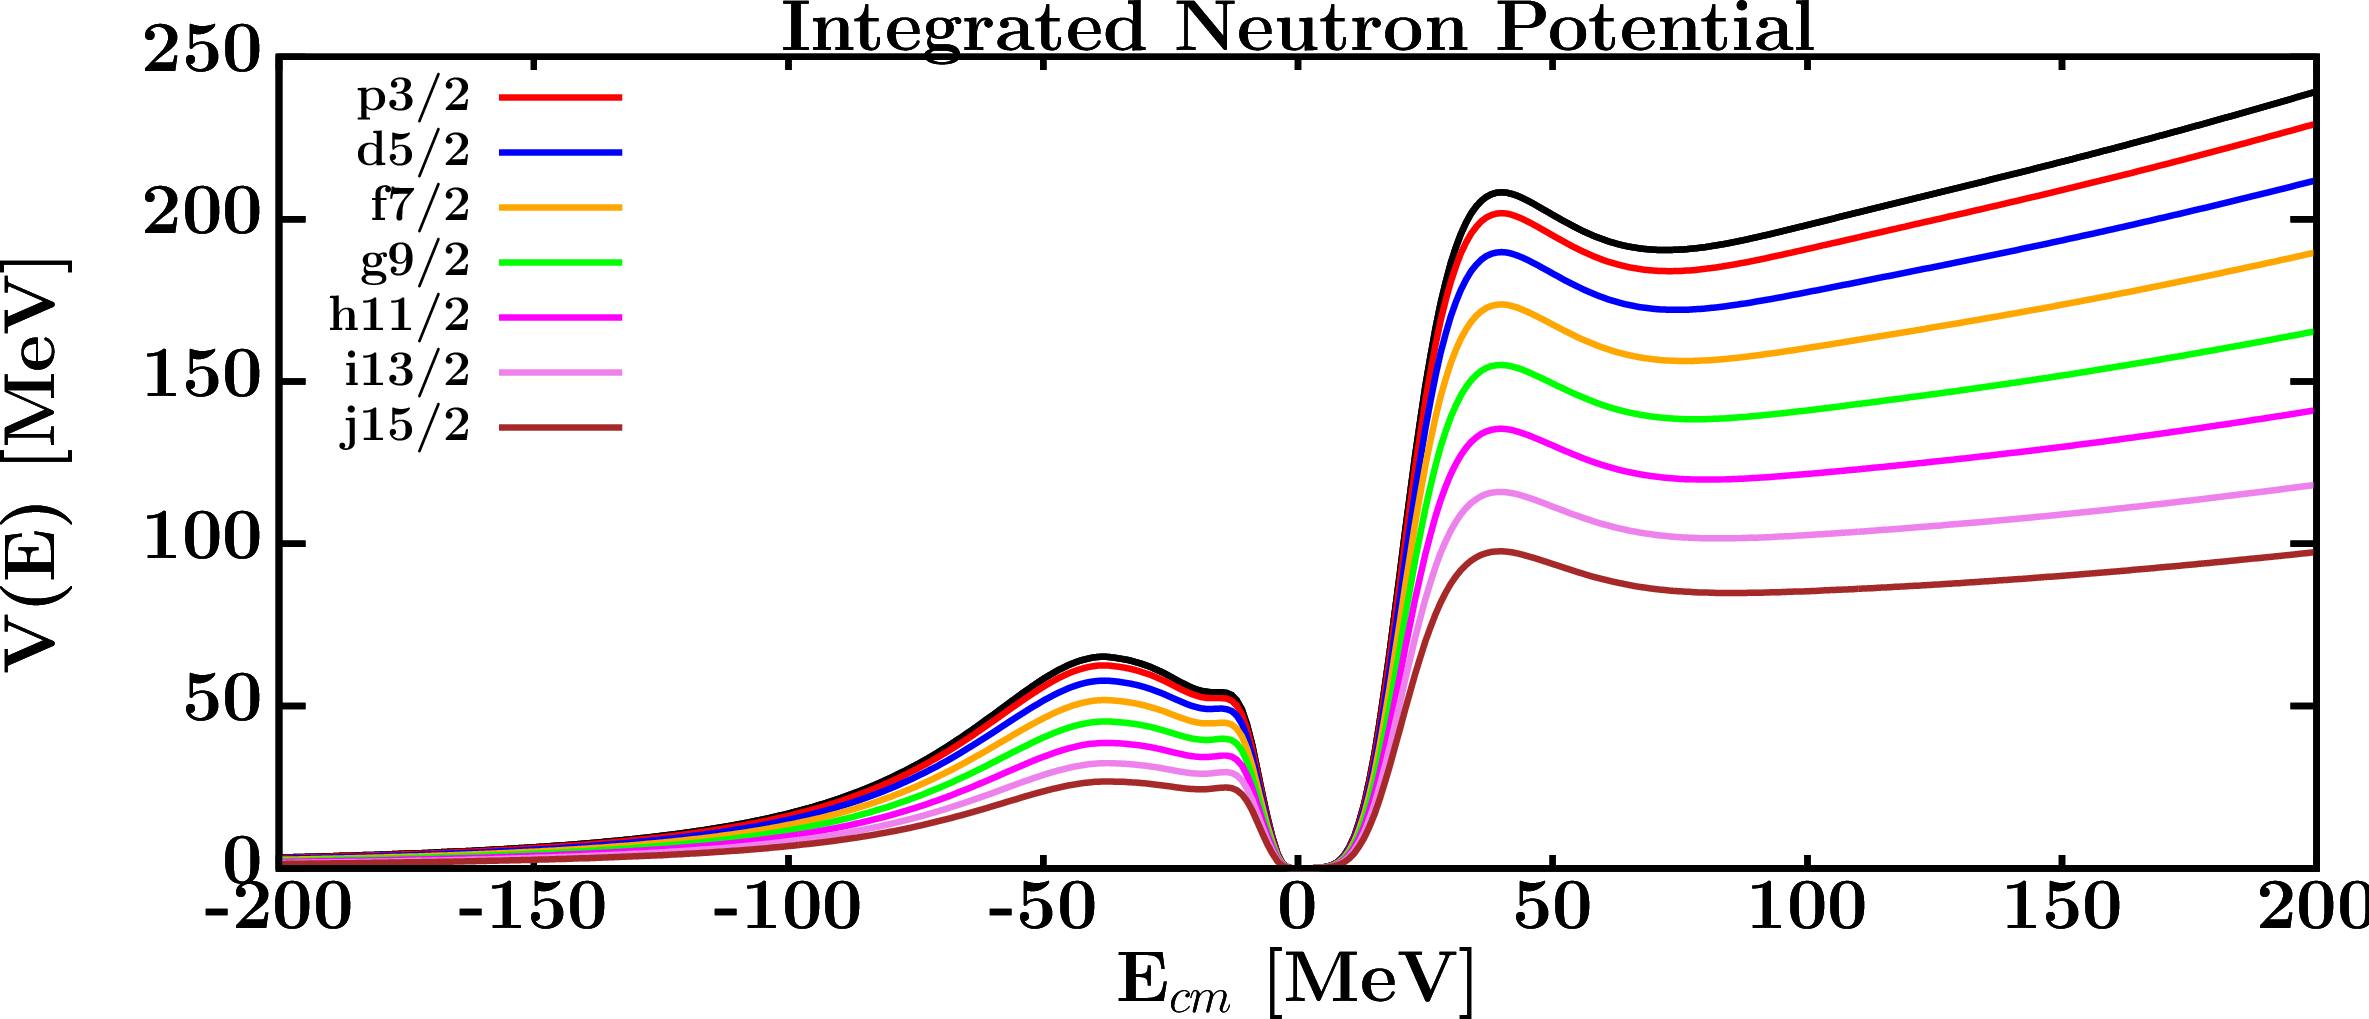
\includegraphics[width=\textwidth]{figures/o18_neutronVolumeIntegrals.png}
        \caption*{\oEight\ neutron volume integral}
        \label{DOMFitData_o18_neutron_potentialIntegral}
    \end{minipage}
\end{figure}
%\vspace{0.3in}
\begin{figure}[hbtp]
    \centering
    \begin{minipage}{0.42\textwidth}
        \centering
        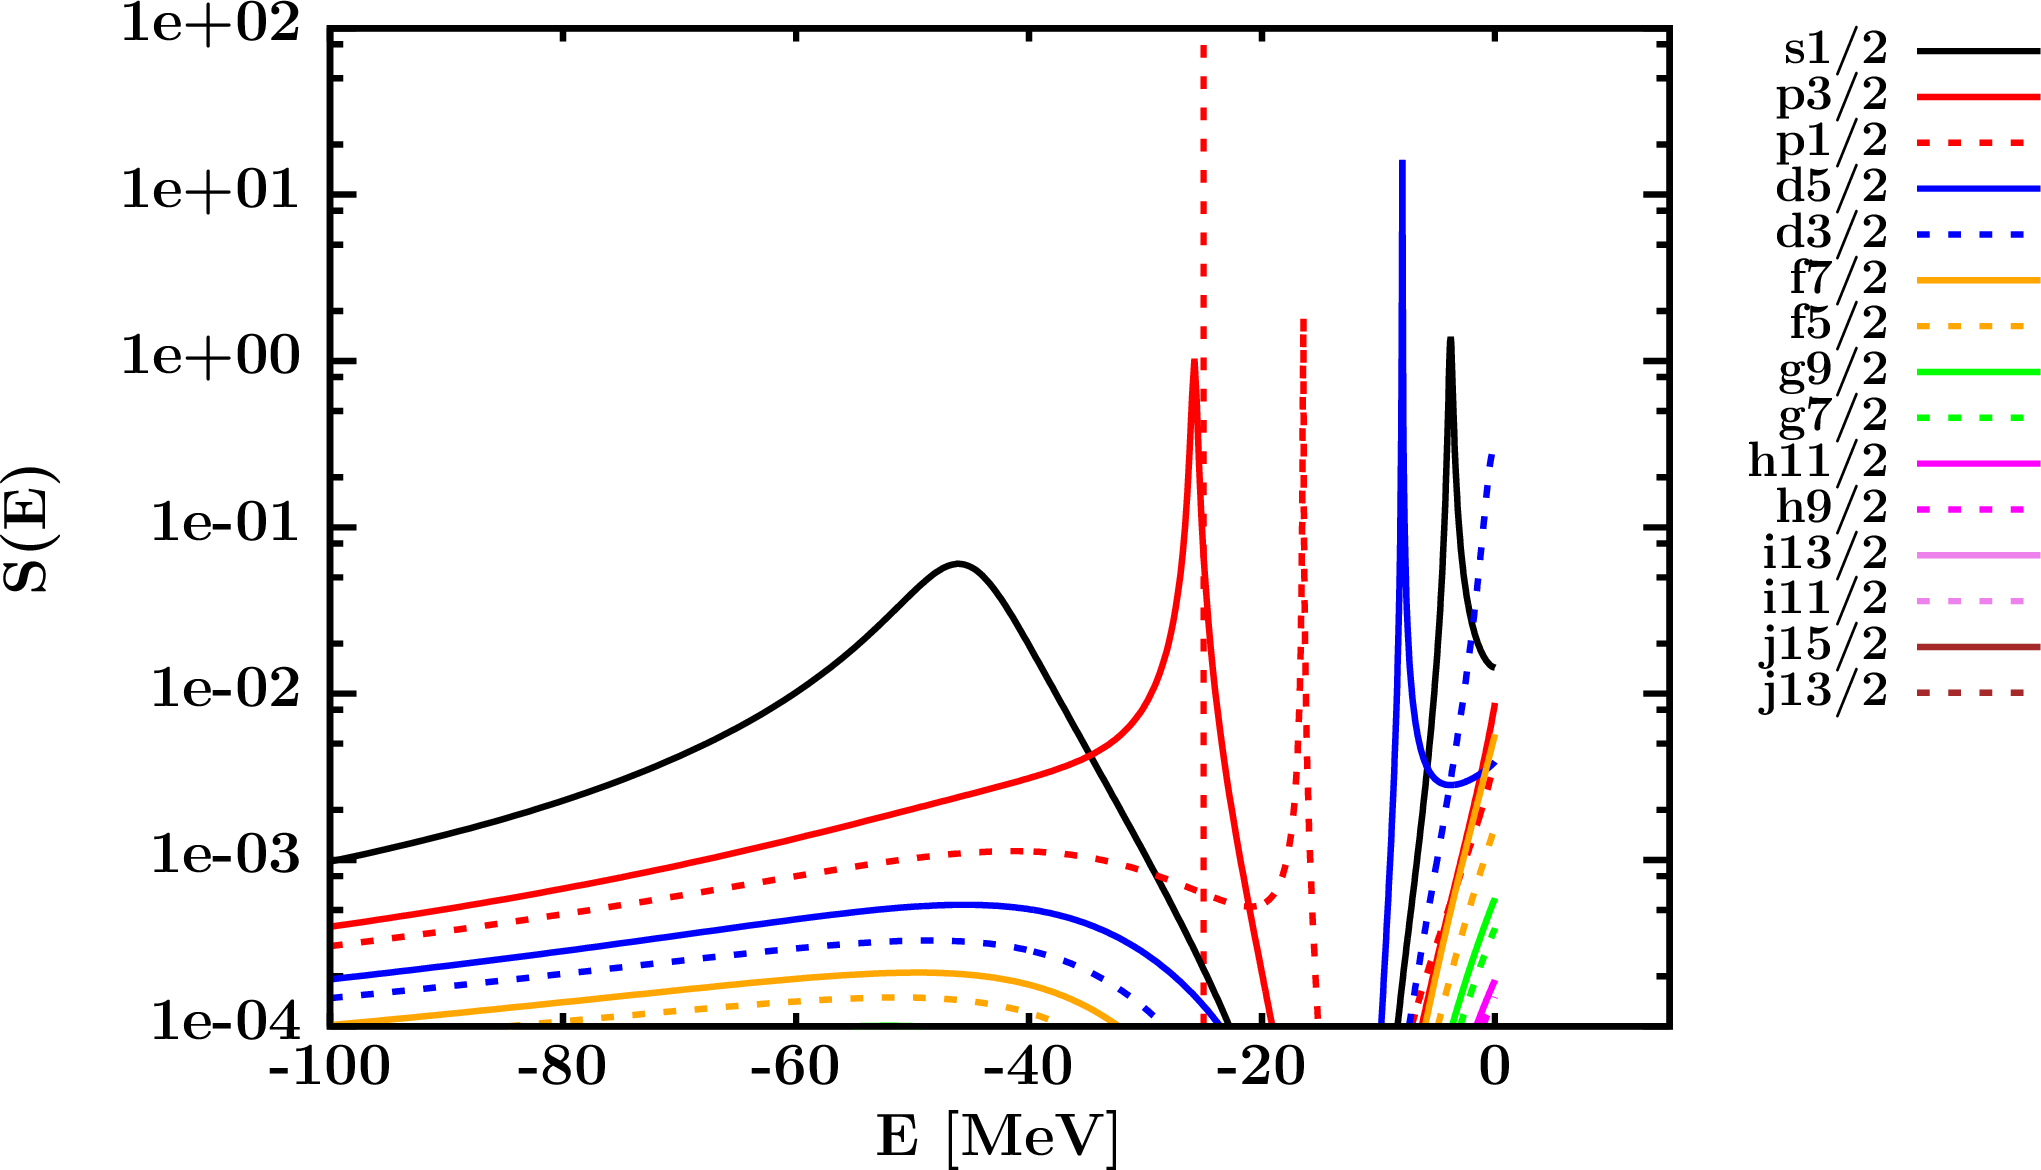
\includegraphics[width=\textwidth]{figures/o18_protonSpectralFunctions.png}
        \caption*{\oEight\ proton spectral functions}
        \label{DOMFitData_o18_proton_spectralFunctions}
    \end{minipage}\hspace{6pt}
    \begin{minipage}{0.42\textwidth}
        \centering
        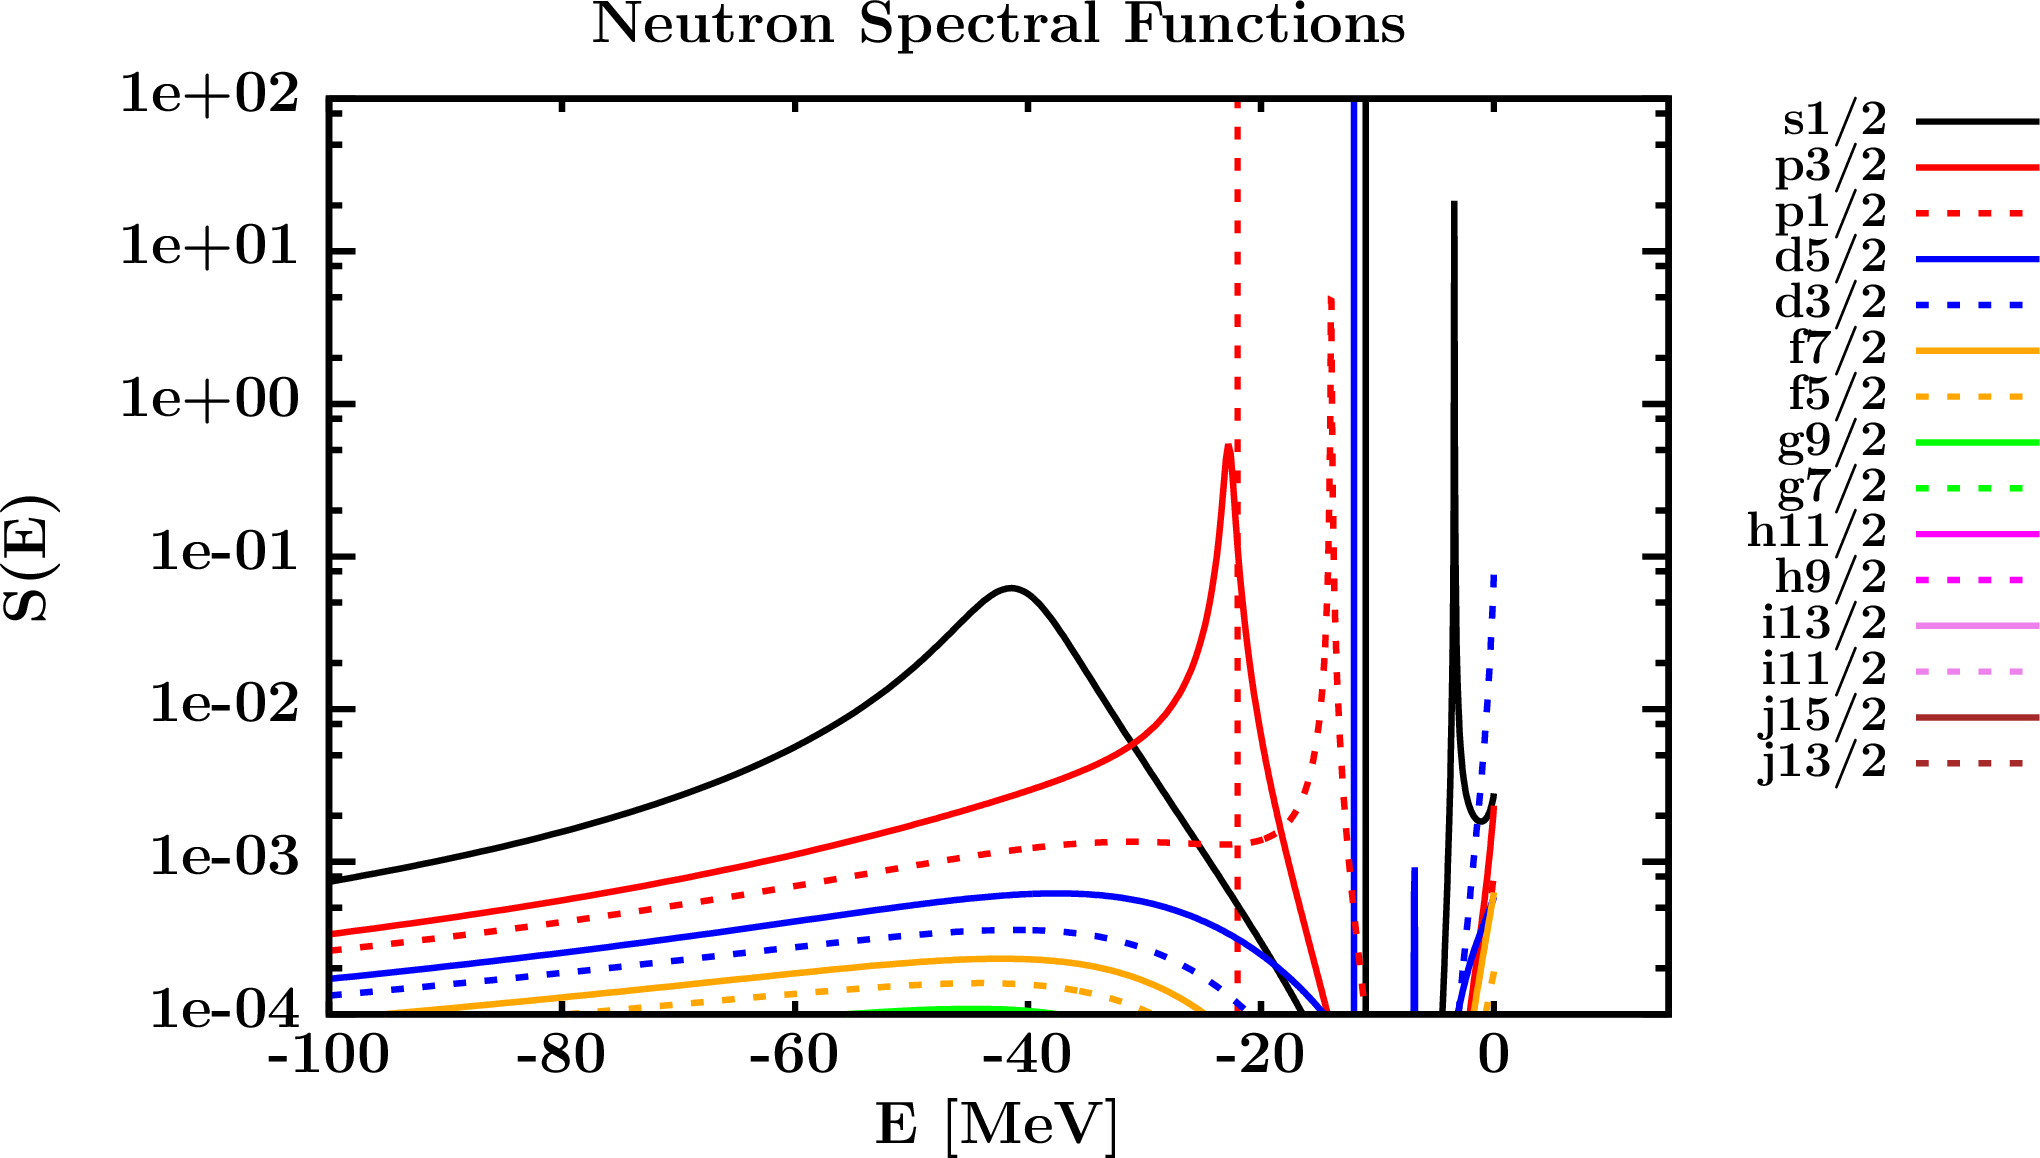
\includegraphics[width=\linewidth]{figures/o18_neutronSpectralFunctions.png}
        \caption*{\oEight\ neutron spectral functions}
        \label{DOMFitData_o18_neutron_spectralFunctions}
    \end{minipage}
\end{figure}
%\afterpage{\clearpage}
\begin{figure}[hbtp]
    \centering
    \begin{minipage}{0.45\textwidth}
        \centering
        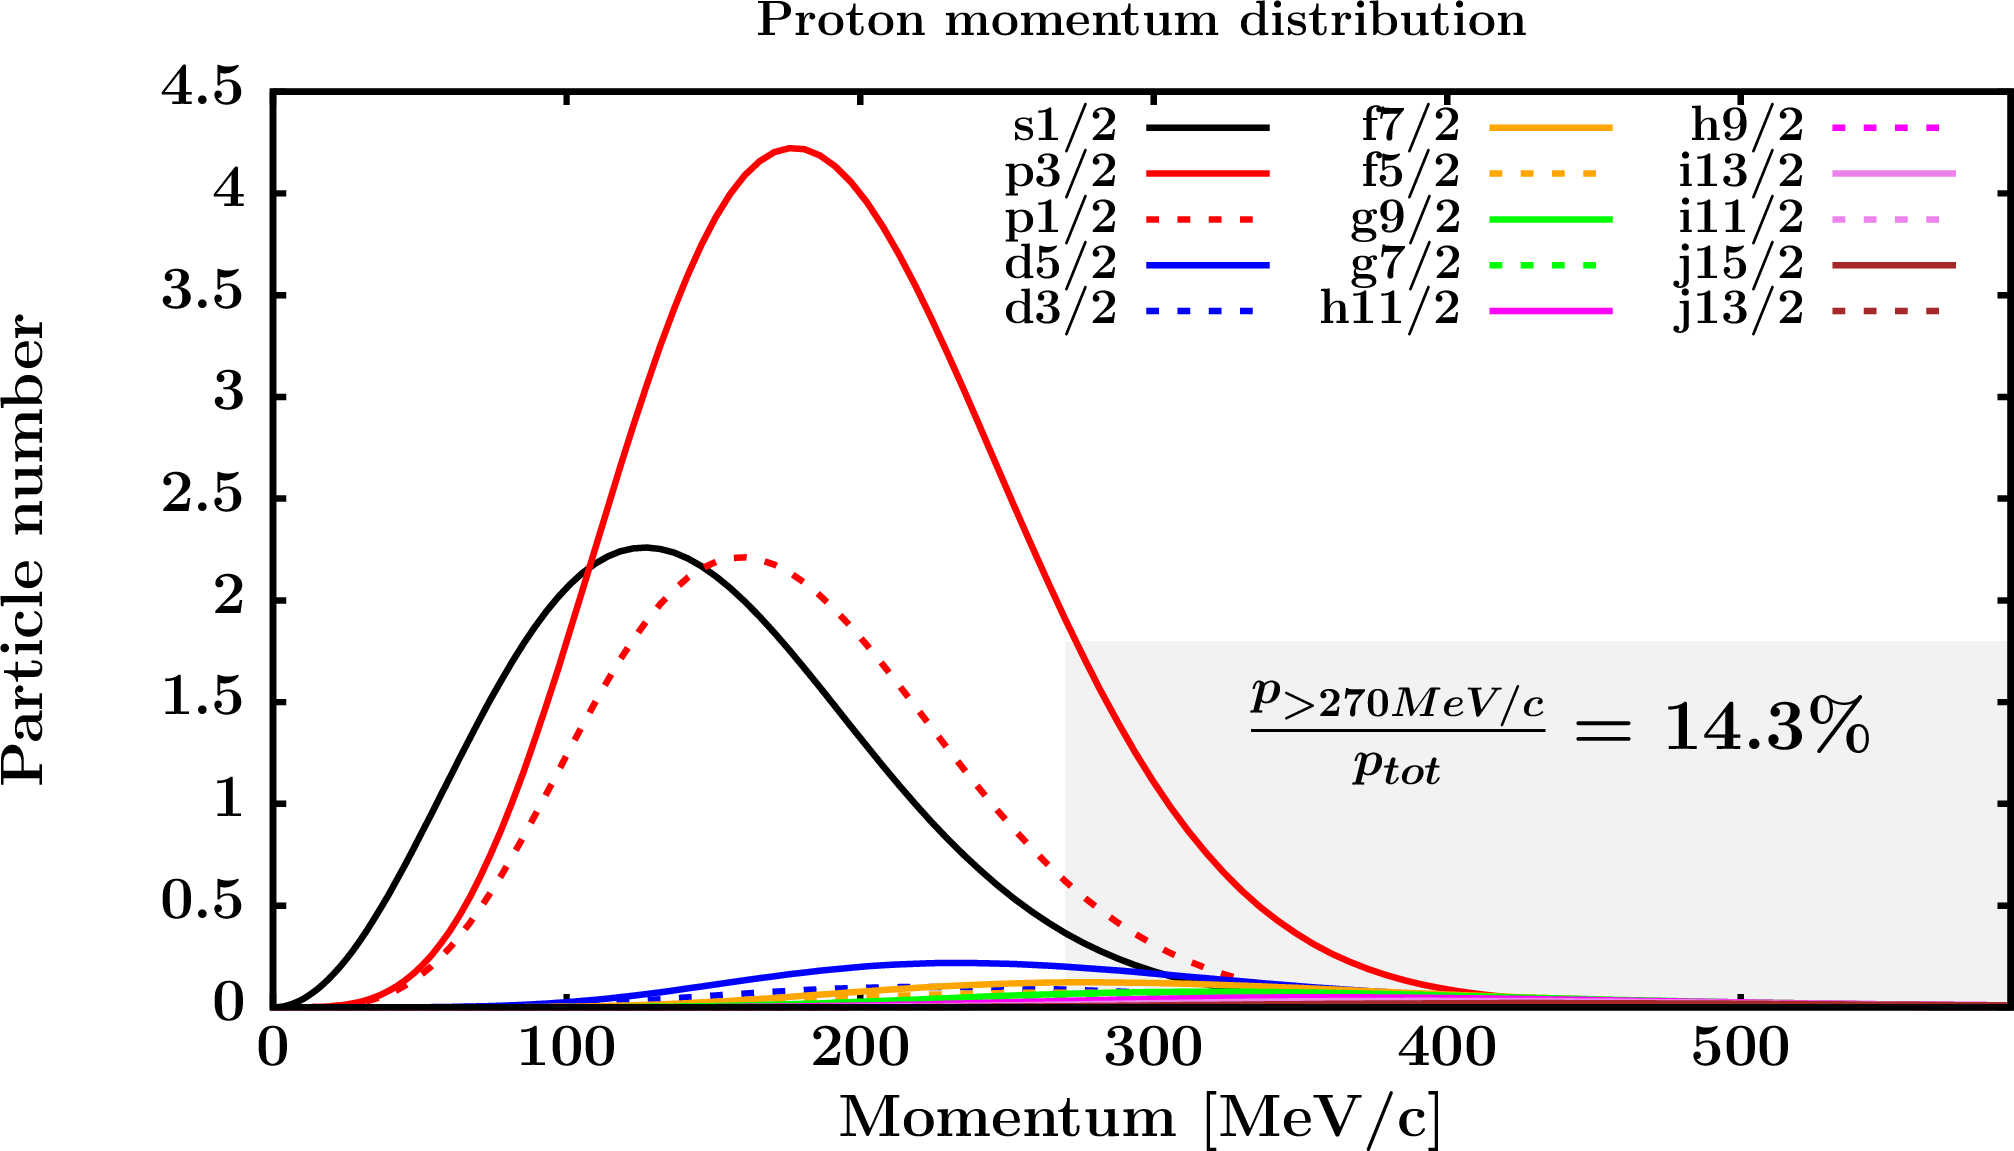
\includegraphics[width=\textwidth]{figures/o18_protonLJMomentumDistIntegral.png}
        \caption*{\oEight\ proton momentum distribution}
        \label{DOMFitData_o18_proton_momentumDist}
    \end{minipage}\hspace{6pt}
    \begin{minipage}{0.45\textwidth}
        \centering
        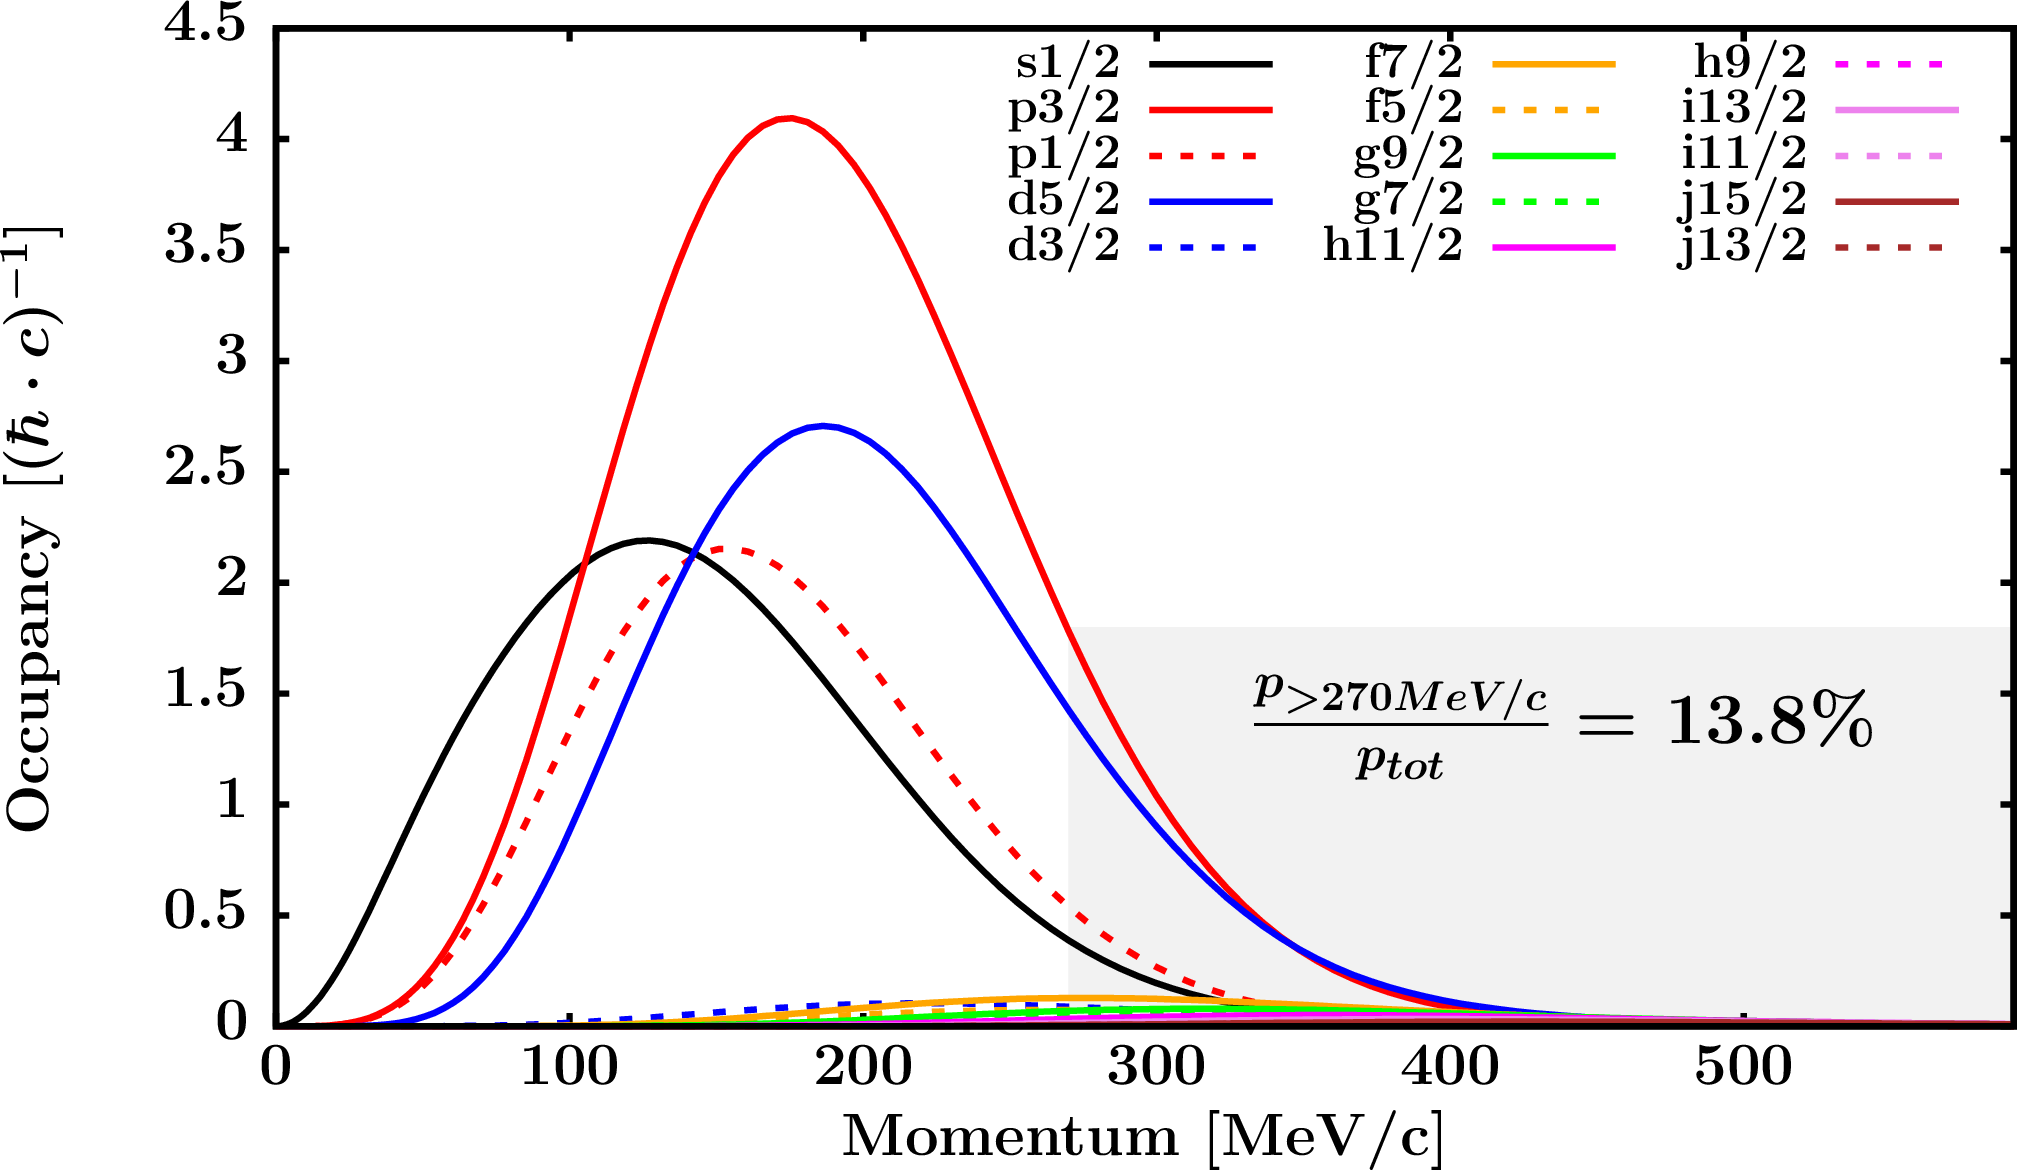
\includegraphics[width=\textwidth]{figures/o18_neutronLJMomentumDistIntegral.png}
        \caption*{\oEight\ neutron momentum distribution}
        \label{DOMFitData_o18_neutron_momentumDist}
    \end{minipage}
\end{figure}
\vspace{0.3in}
\begin{figure}[hbtp]
    \centering
    \begin{minipage}{0.45\textwidth}
        \centering
        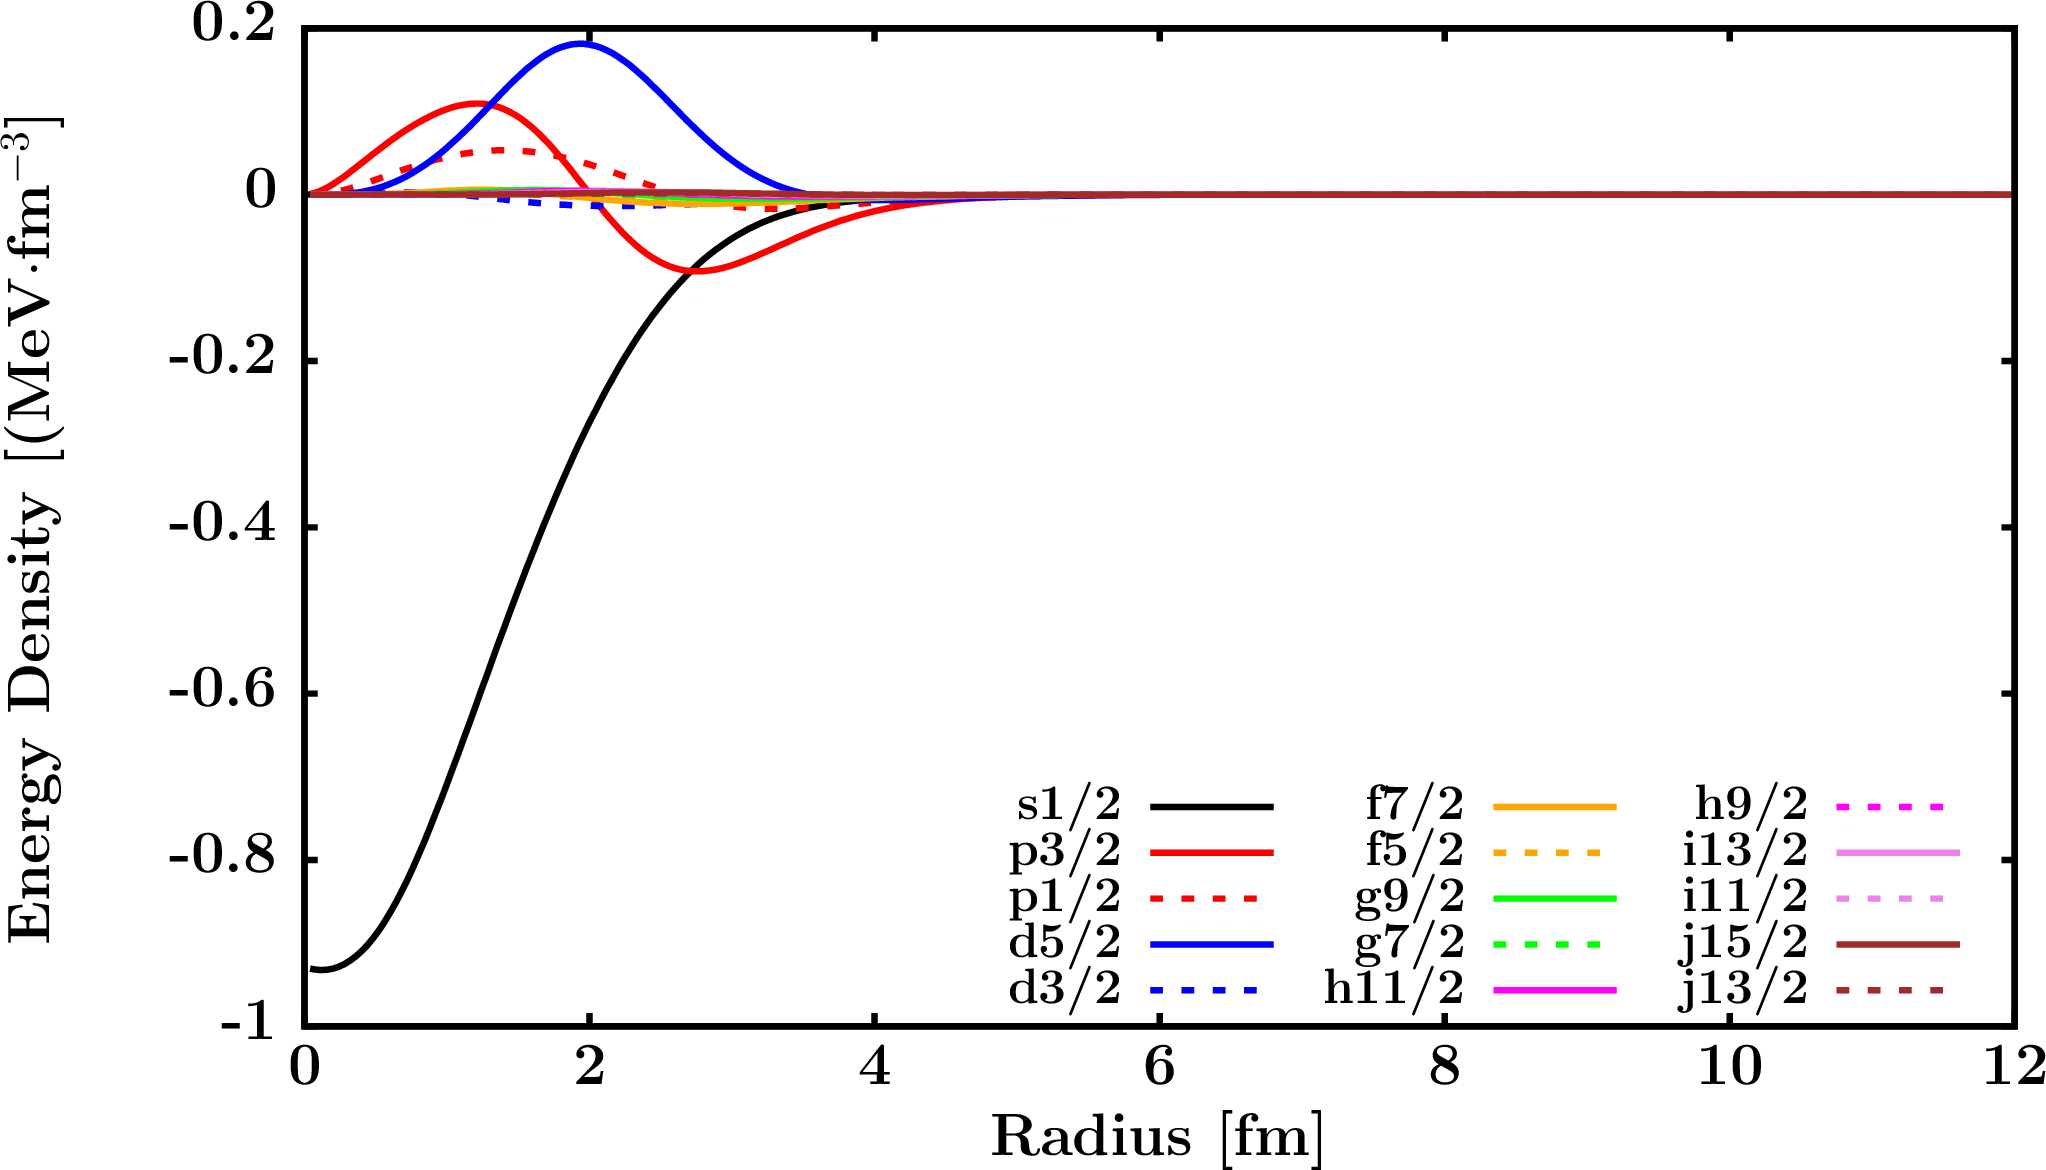
\includegraphics[width=\textwidth]{figures/o18_EnergyDist.png}
        \caption*{\oEight\ energy distribution by LJ}
        \label{DOMFitData_o18_proton_energyDistInt}
    \end{minipage}\hspace{6pt}
    \begin{minipage}{0.45\textwidth}
        \centering
        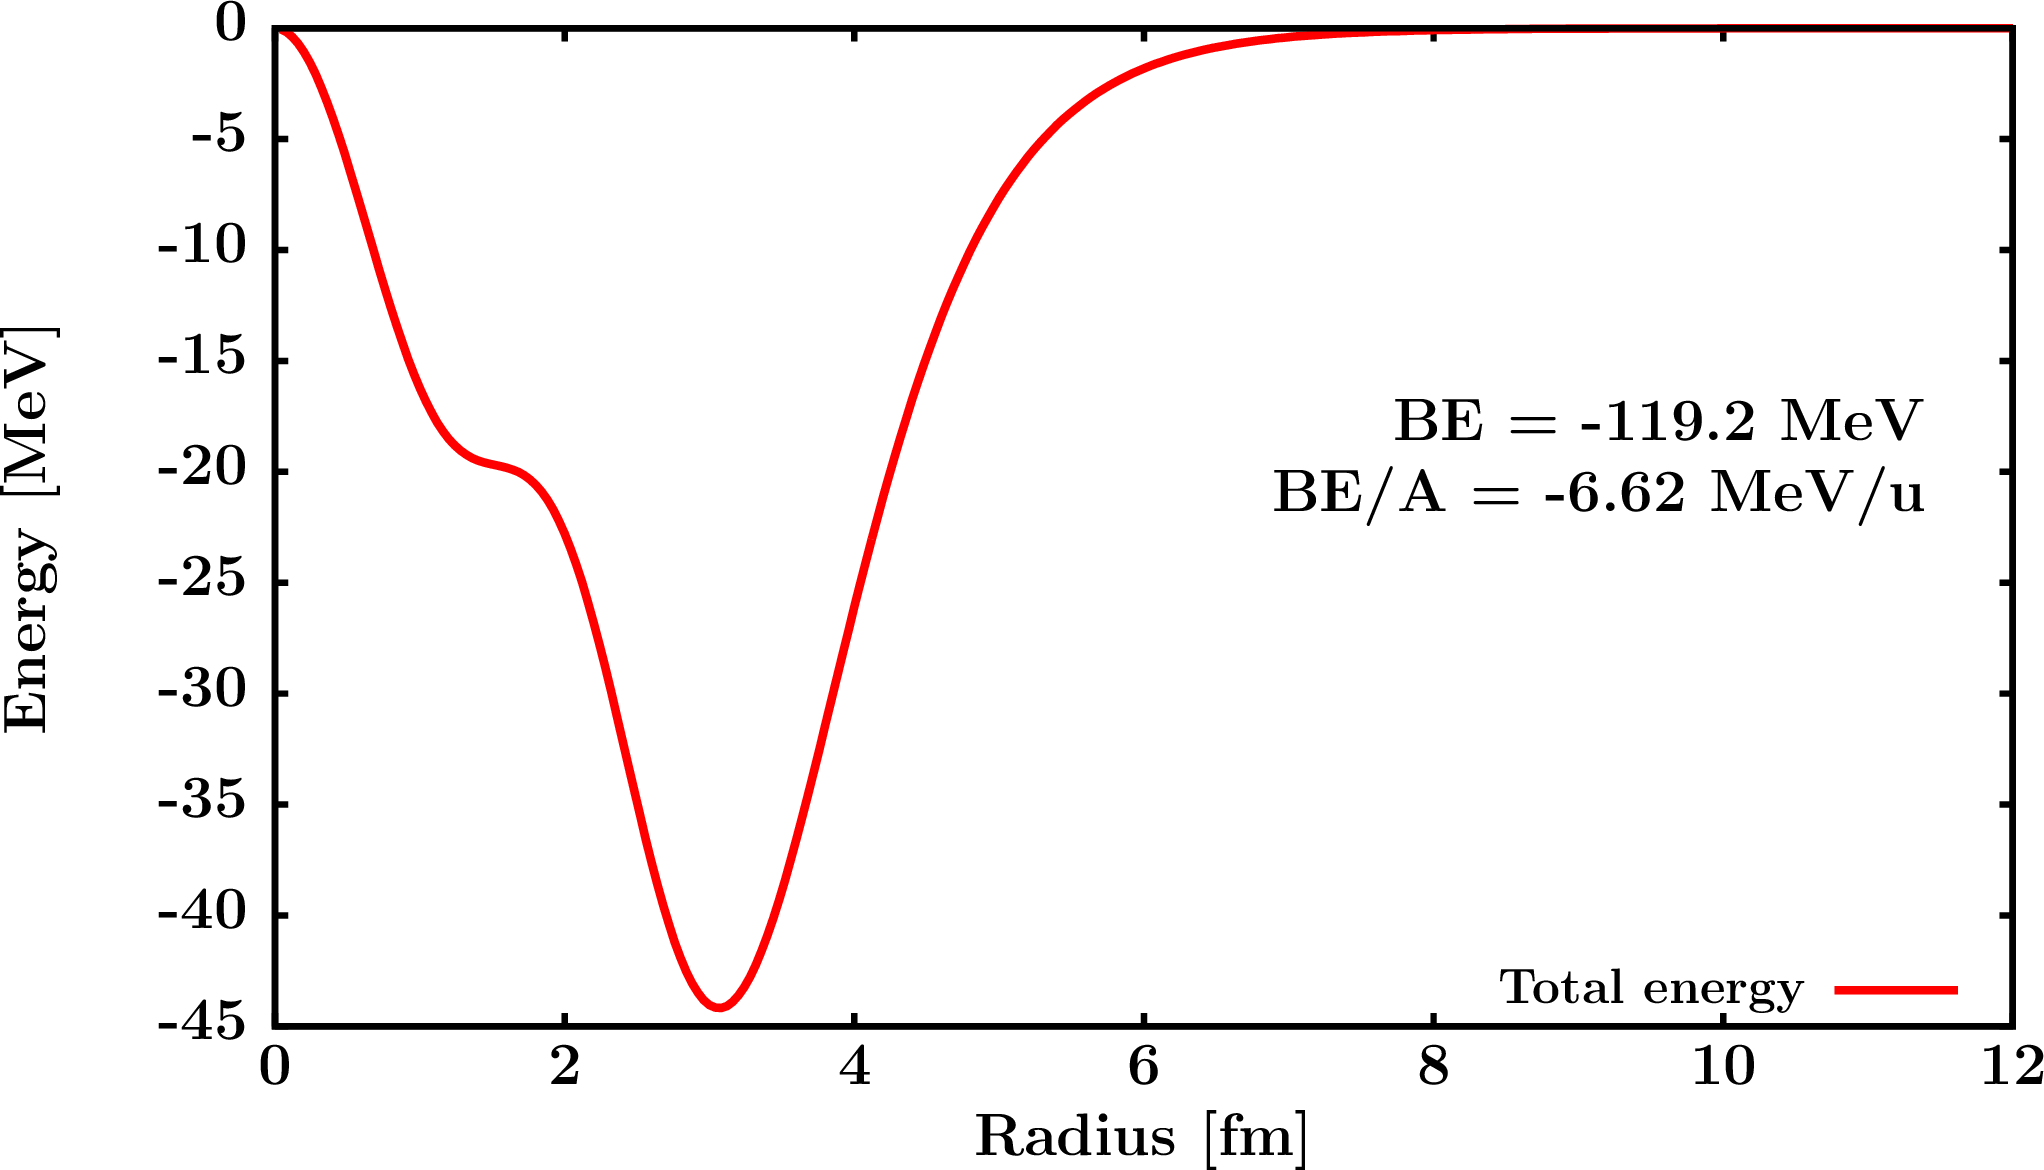
\includegraphics[width=\textwidth]{figures/o18_EnergyDistIntegral.png}
        \caption*{\oEight\ energy distribution integral}
        \label{DOMFitData_o18_neutron_energyDistInt}
    \end{minipage}
\end{figure}
\vspace{0.4in}
\begin{figure}[hbtp]
    \centering
    \begin{minipage}{0.70\textwidth}
        \centering
        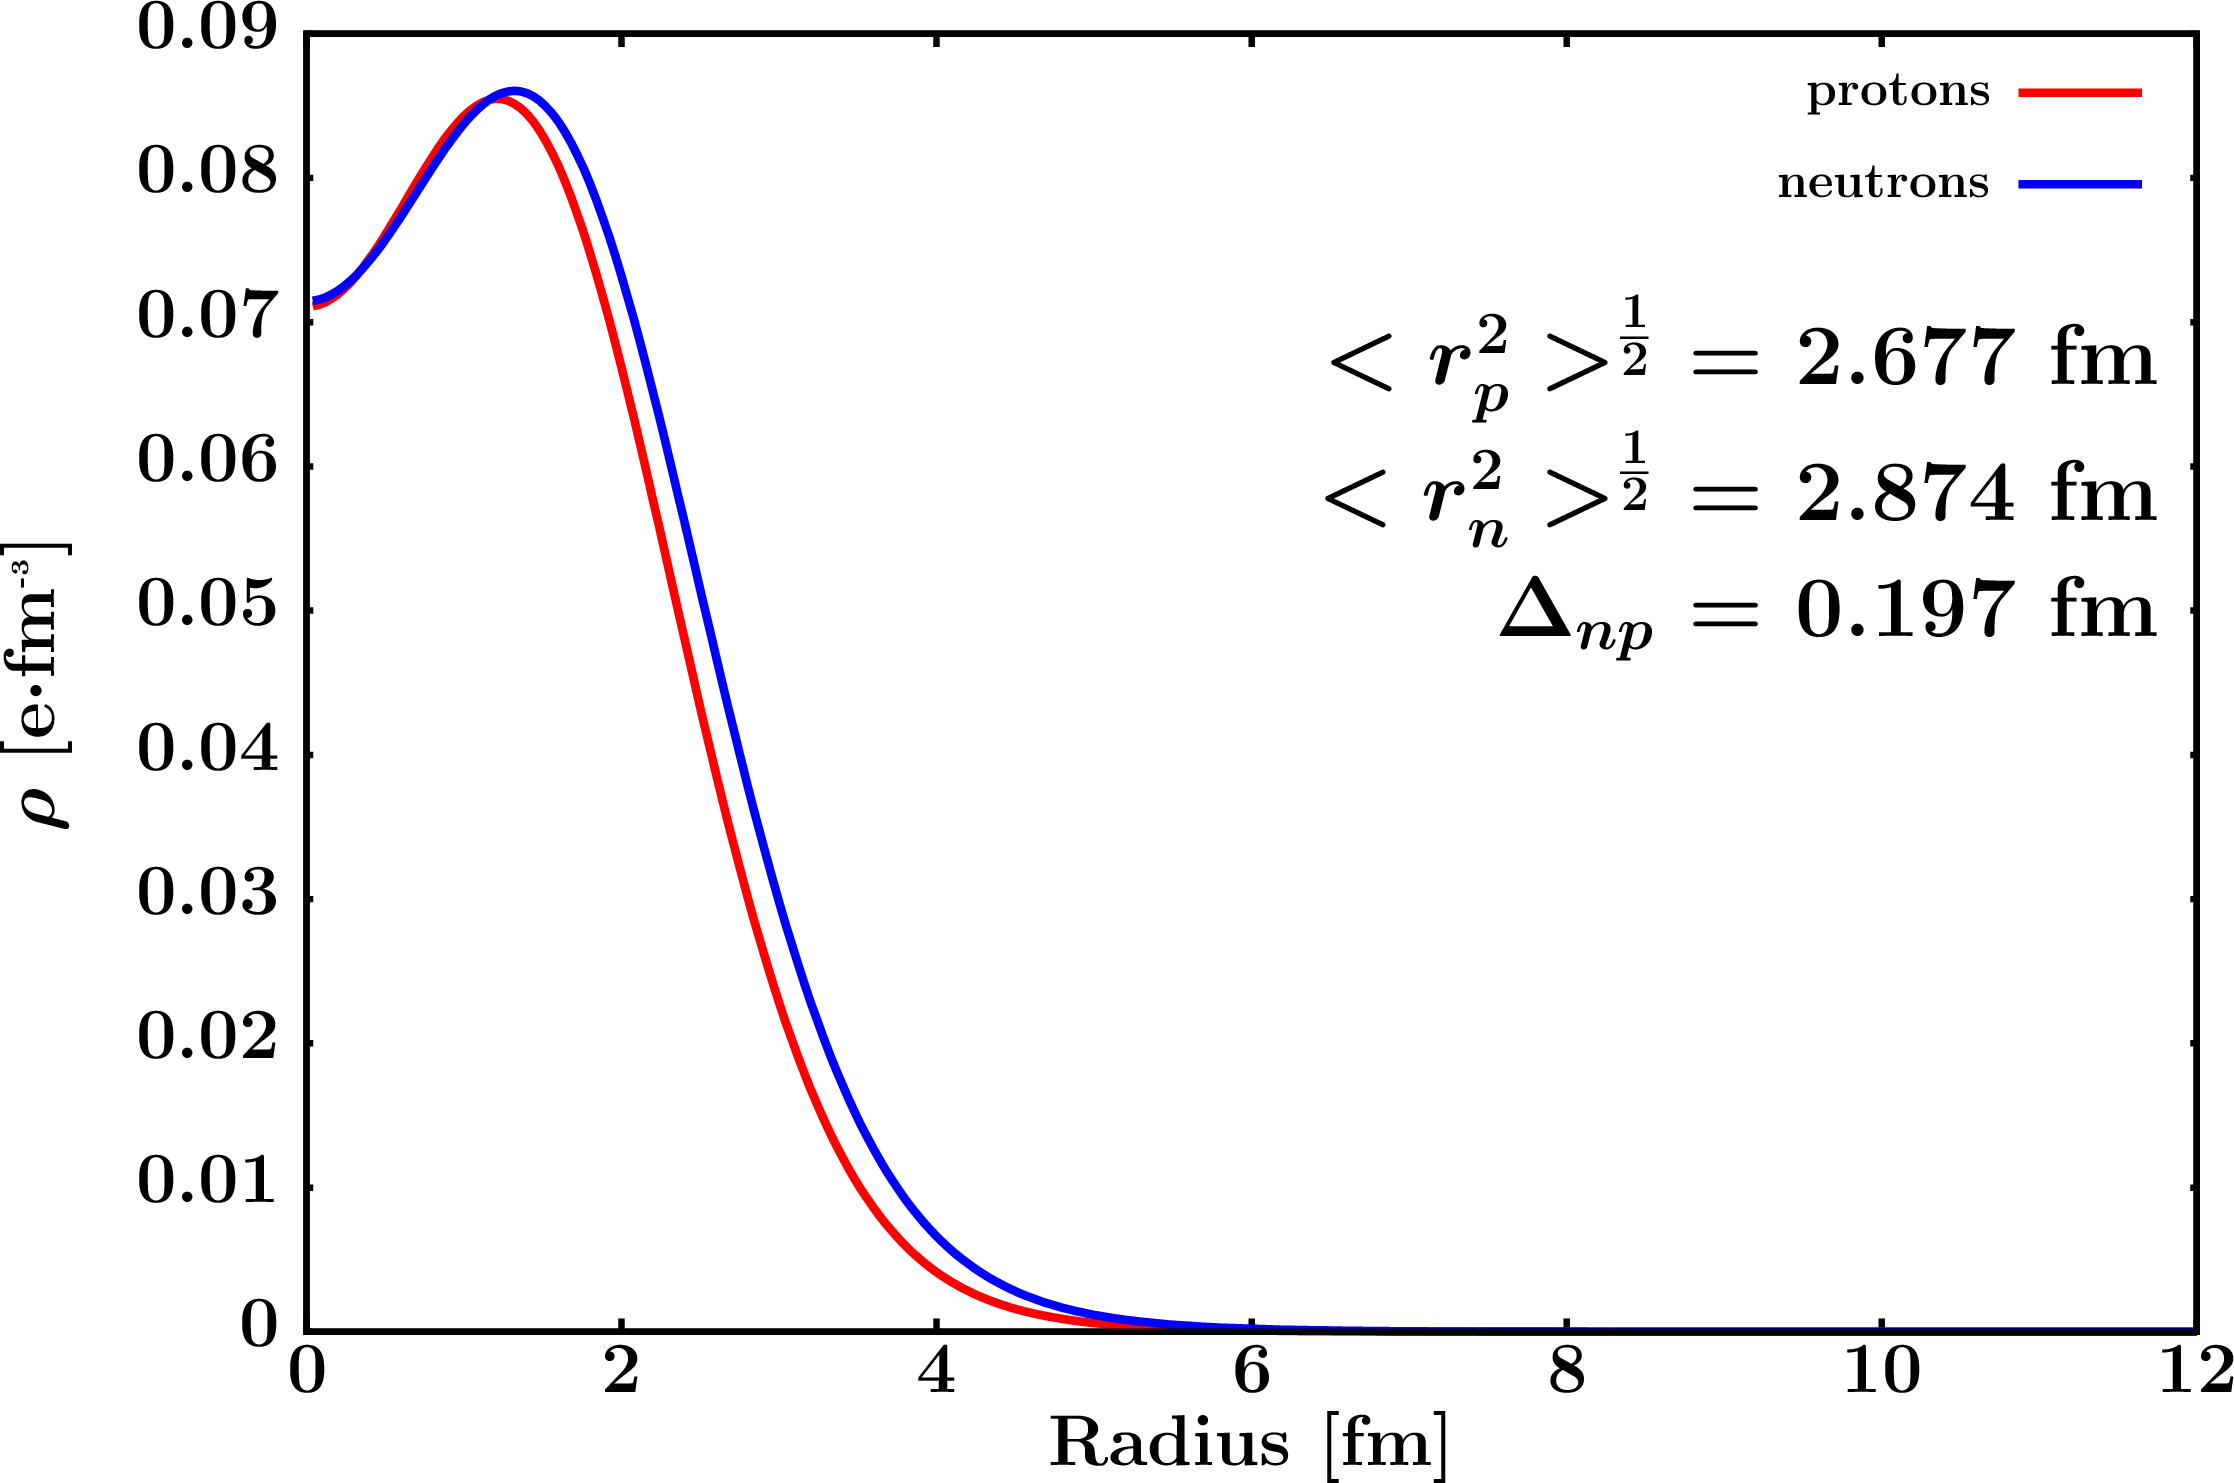
\includegraphics[width=\linewidth]{figures/o18_matterDensity.png}
        \caption*{\oEight\ matter density distribution}
        \label{DOMFitData_o18_matterDensity}
    \end{minipage}
\end{figure}

\section{DOM fit of \caForty}
\label{ca40DOMOutput}
\begin{figure}[hbtp]
    \centering
    \begin{minipage}{0.47\textwidth}
        \centering
        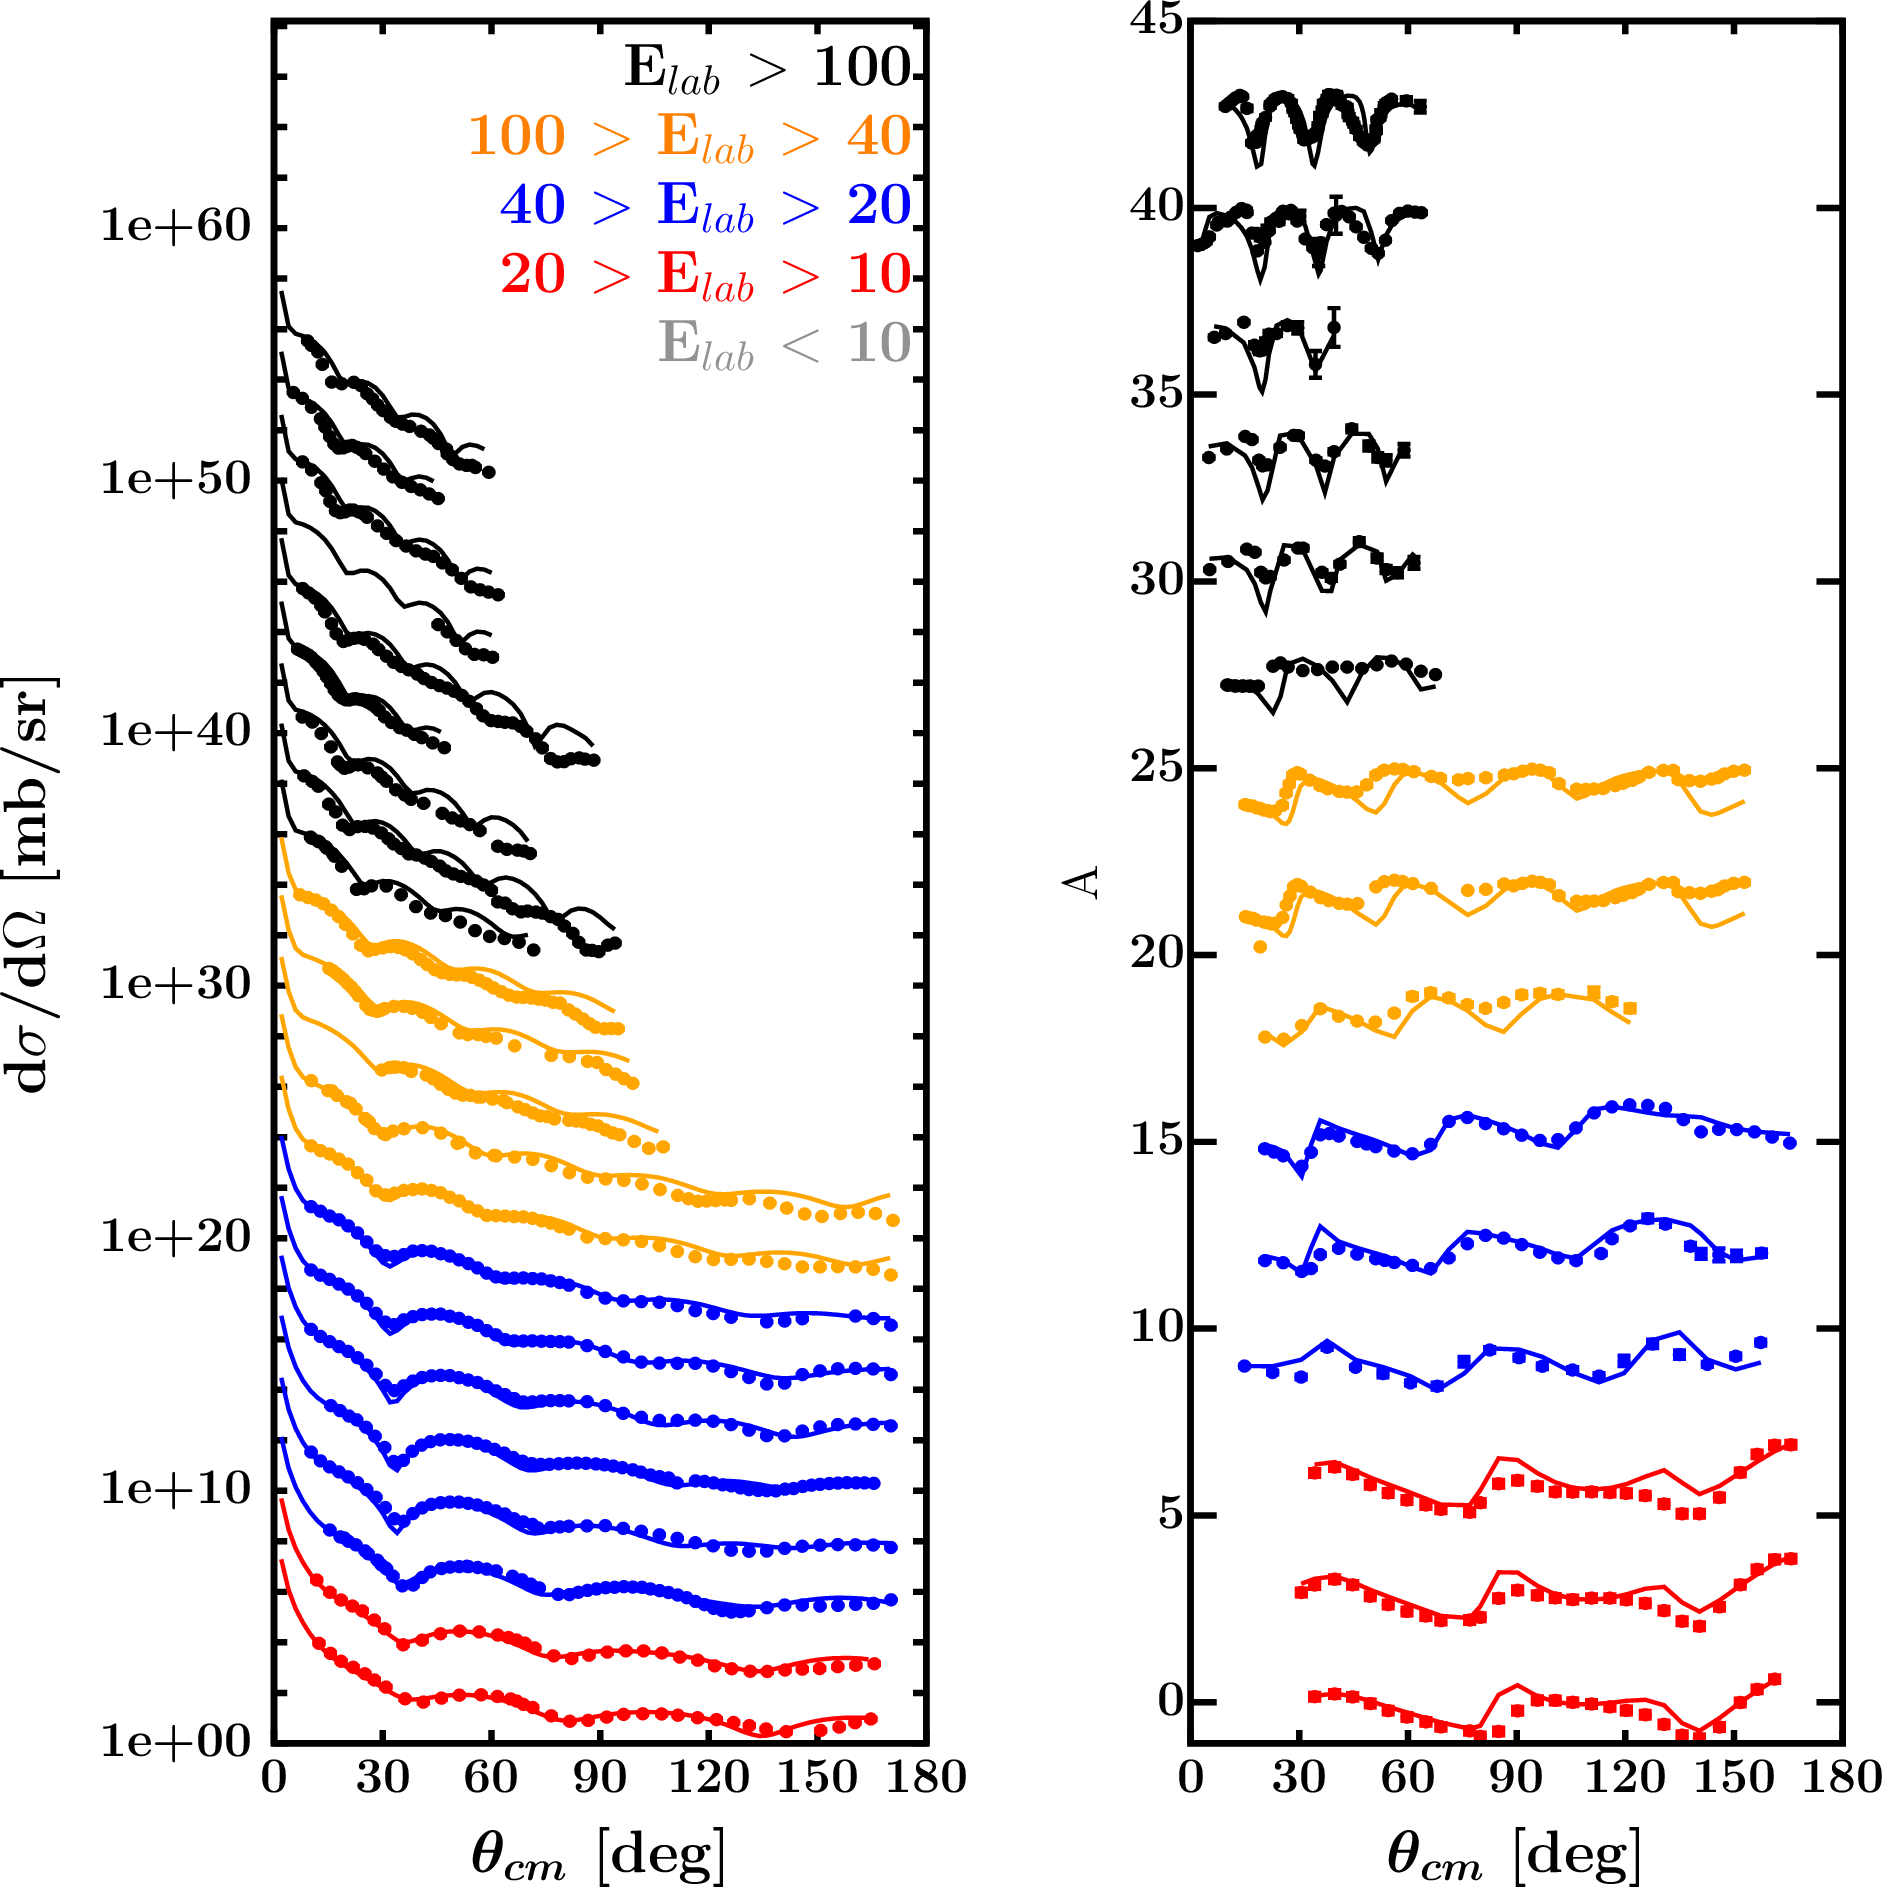
\includegraphics[width=\textwidth]{figures/ca40_protonElastic.png}
        \caption*{\caForty\ proton elastic scattering}
        \label{DOMFitData_ca40_proton_elastic}
    \end{minipage}\hspace{6pt}
    \begin{minipage}{0.47\textwidth}
        \centering
        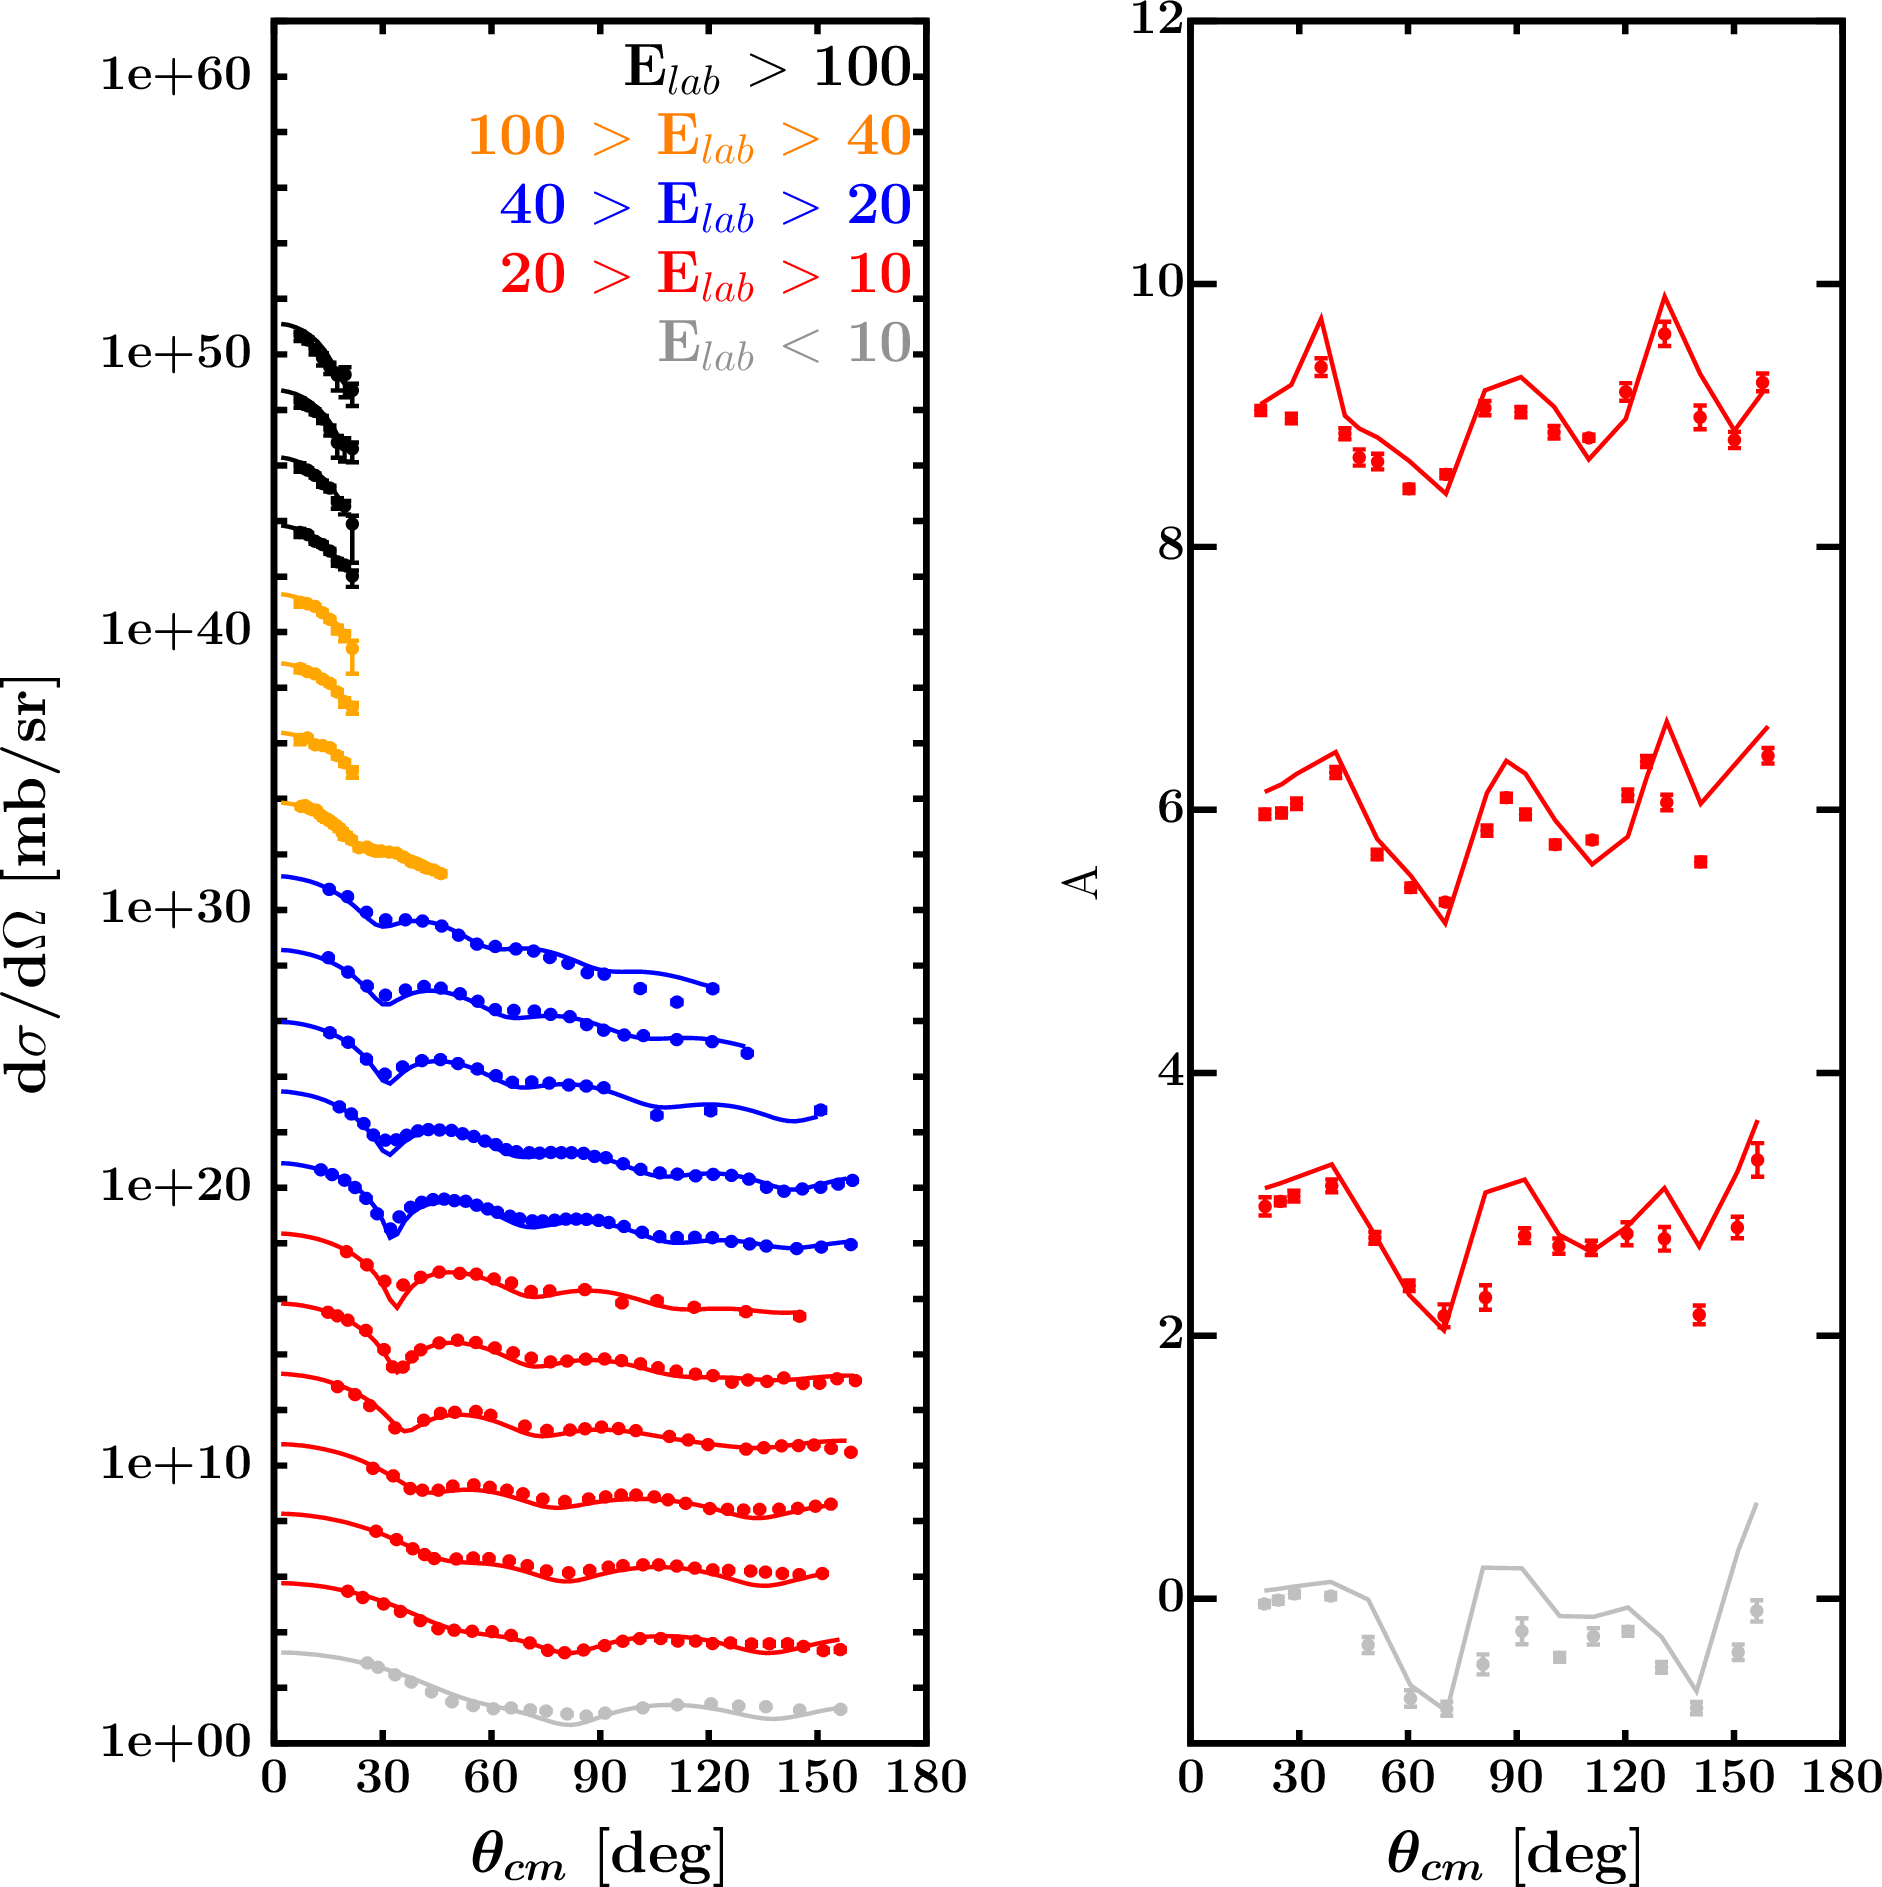
\includegraphics[width=\textwidth]{figures/ca40_neutronElastic.png}
        \caption*{\caForty\ neutron elastic scattering}
        \label{DOMFitData_ca40_neutron_elastic}
    \end{minipage}
\end{figure}
\vspace{0.70in}
\begin{figure}[hbtp]
    \centering
    \begin{minipage}{0.47\textwidth}
        \centering
        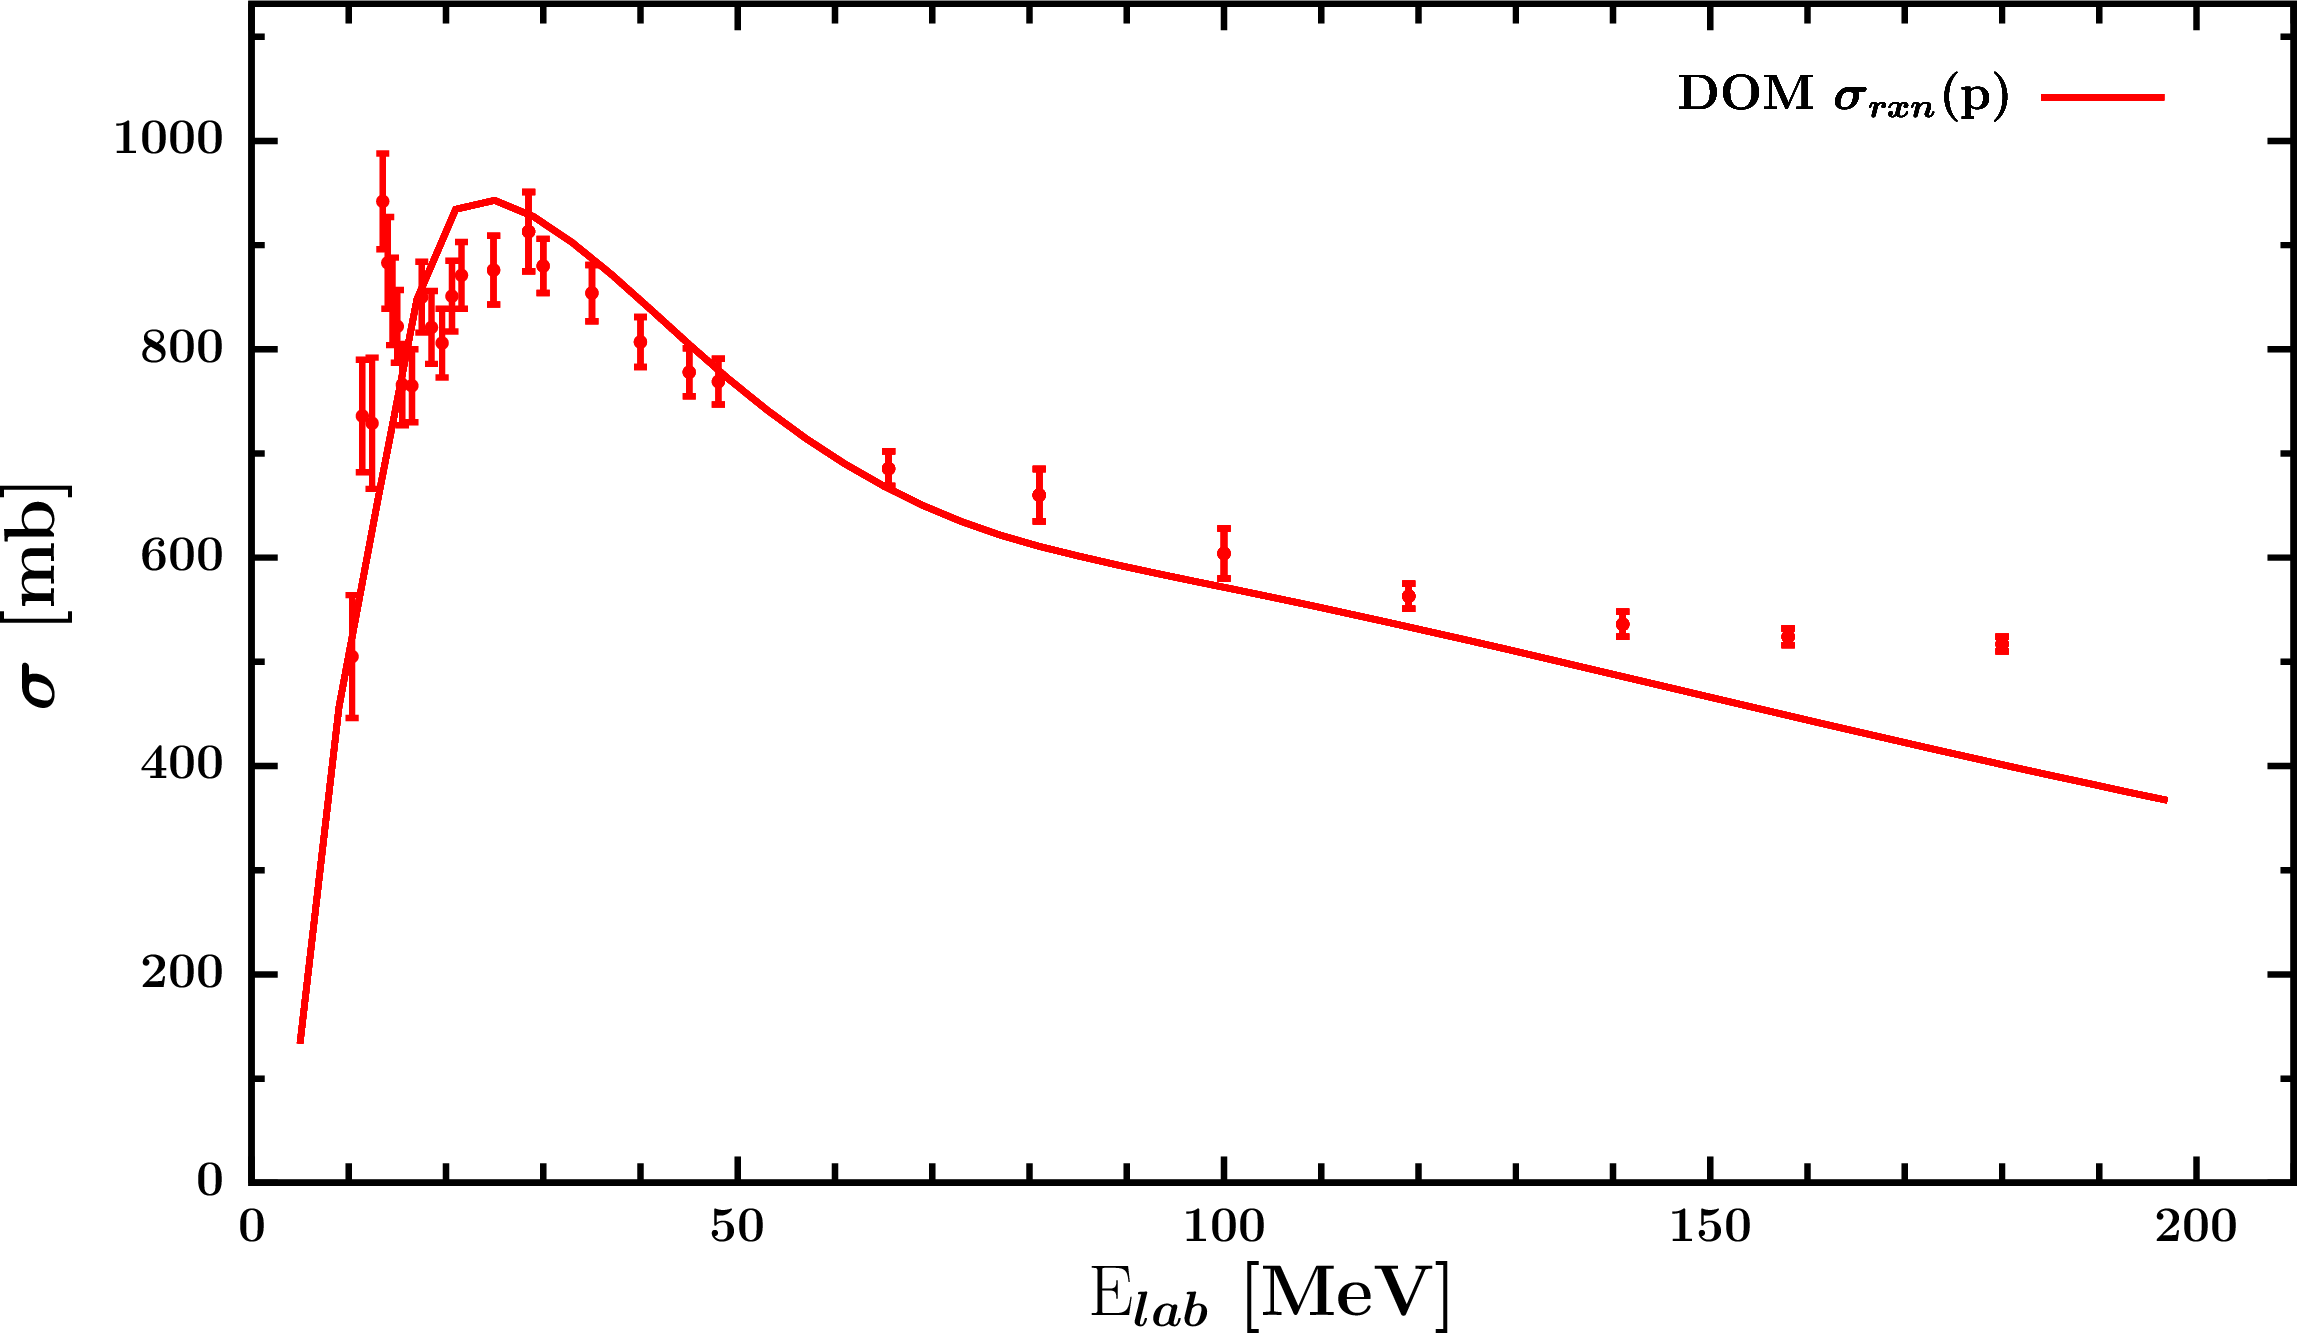
\includegraphics[width=\linewidth]{figures/ca40_protonInelastic.png}
        \caption*{\caForty\ proton \rxn}
        \label{DOMFitData_ca40_proton_inelastic}
    \end{minipage}\hspace{6pt}
    \begin{minipage}{0.47\textwidth}
        \centering
        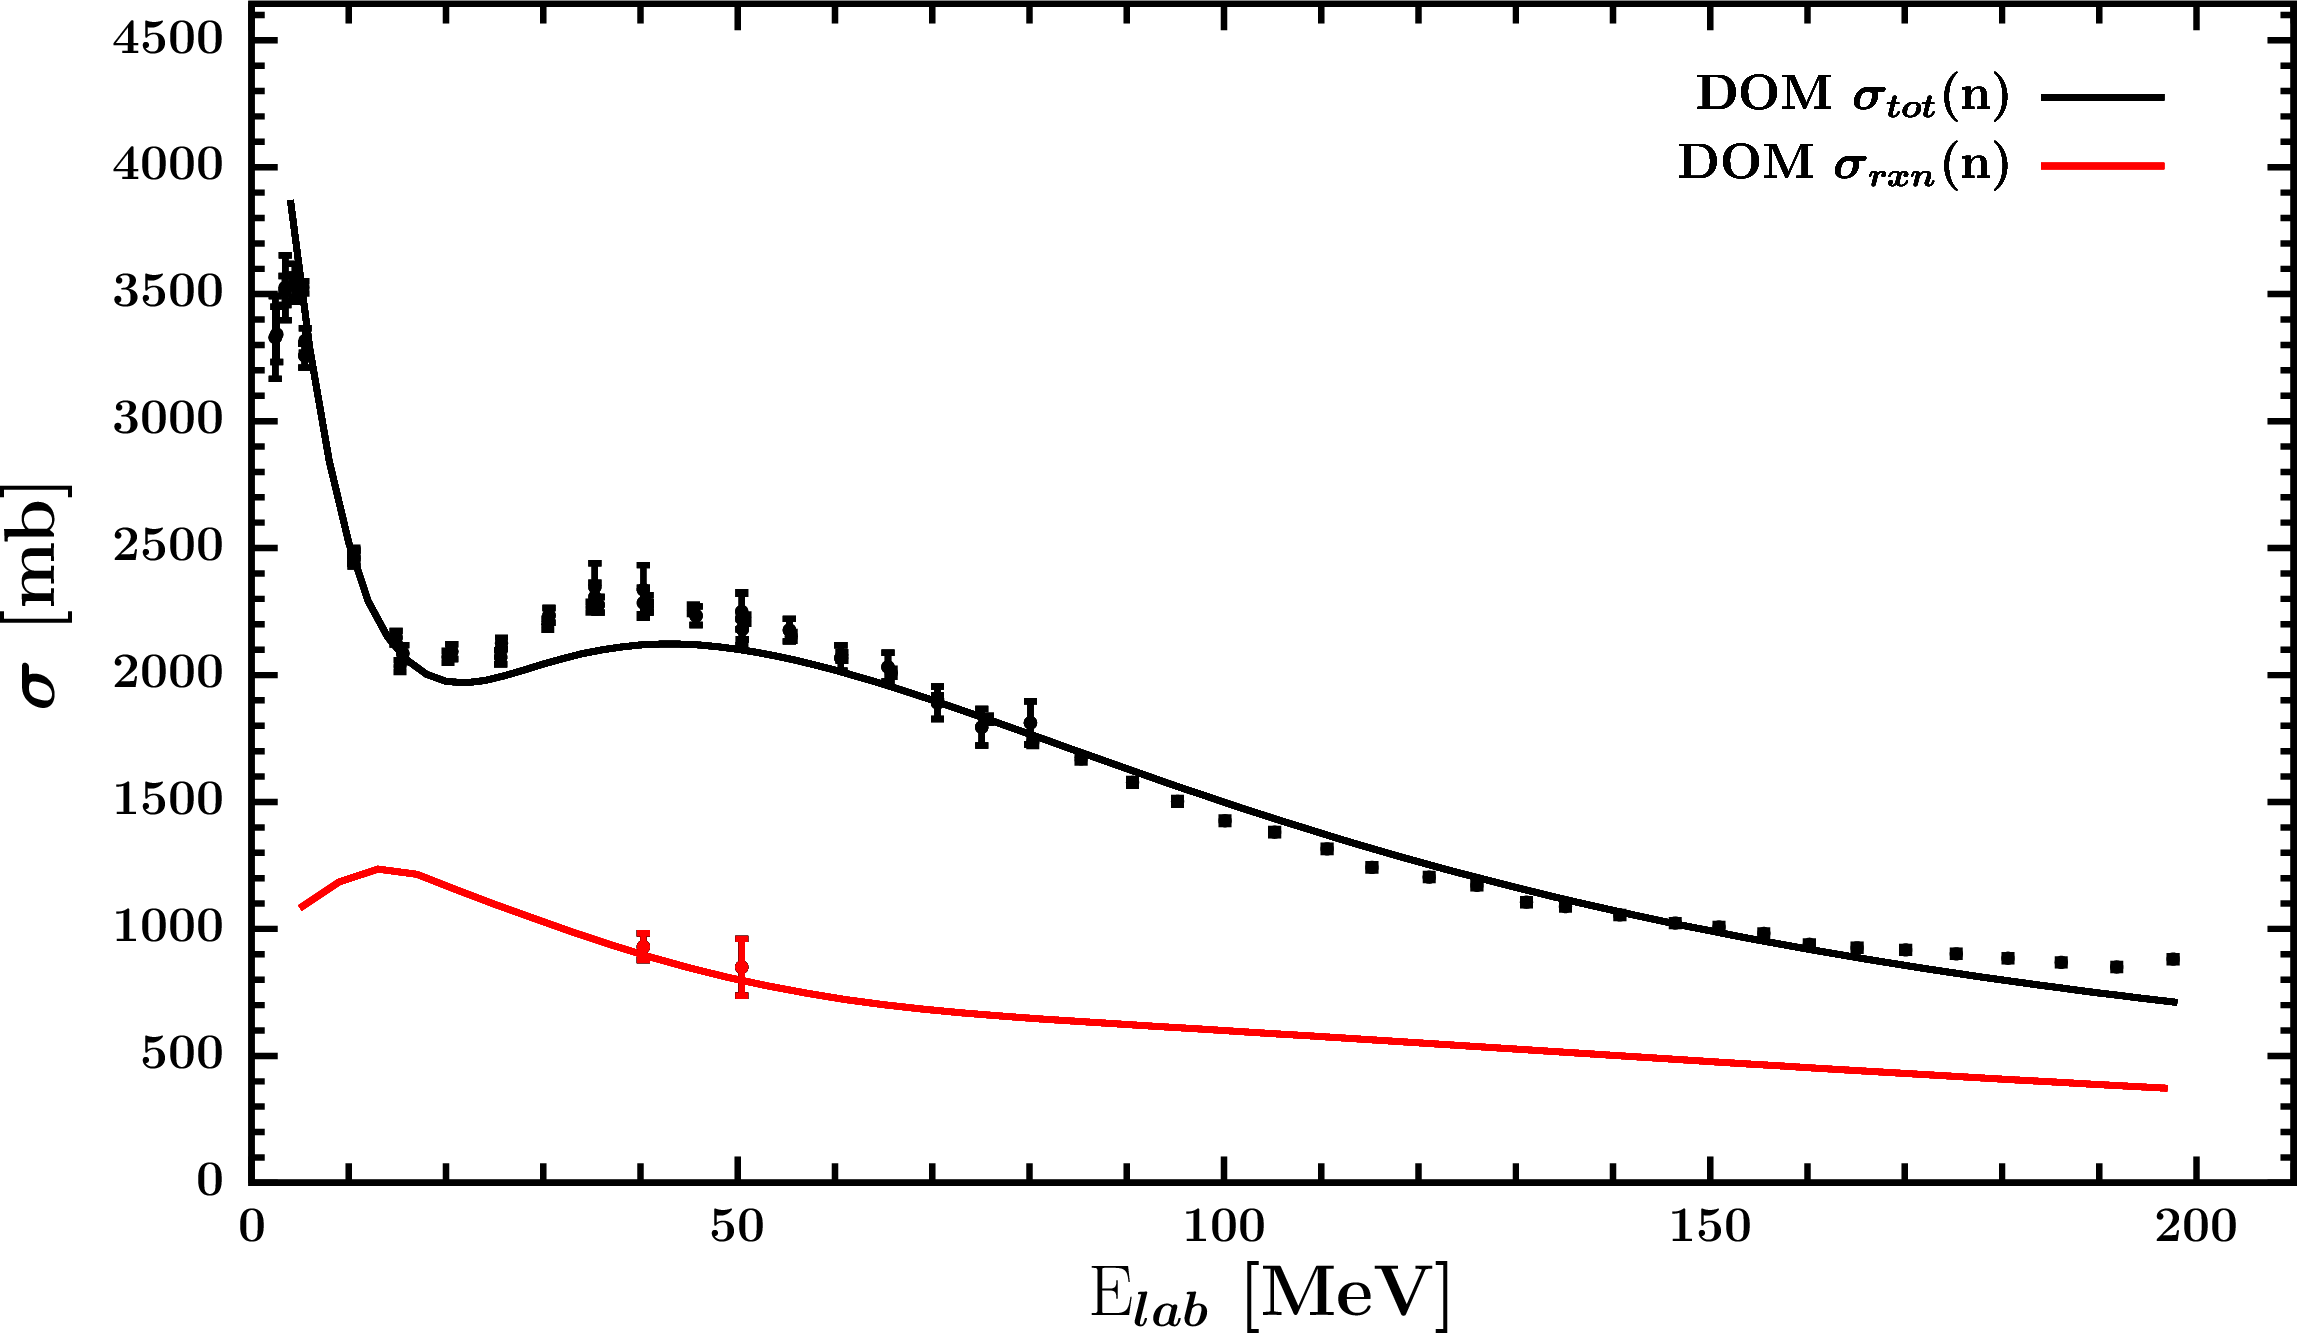
\includegraphics[width=\textwidth]{figures/ca40_neutronInelastic.png}
        \caption*{\caForty\ neutron \rxn\ and \tot}
        \label{DOMFitData_ca40_neutron_inelastic}
    \end{minipage}
\end{figure}
%\afterpage{\clearpage}
\begin{figure}[hbtp]
    \centering
    \begin{minipage}{0.42\textwidth}
        \centering
        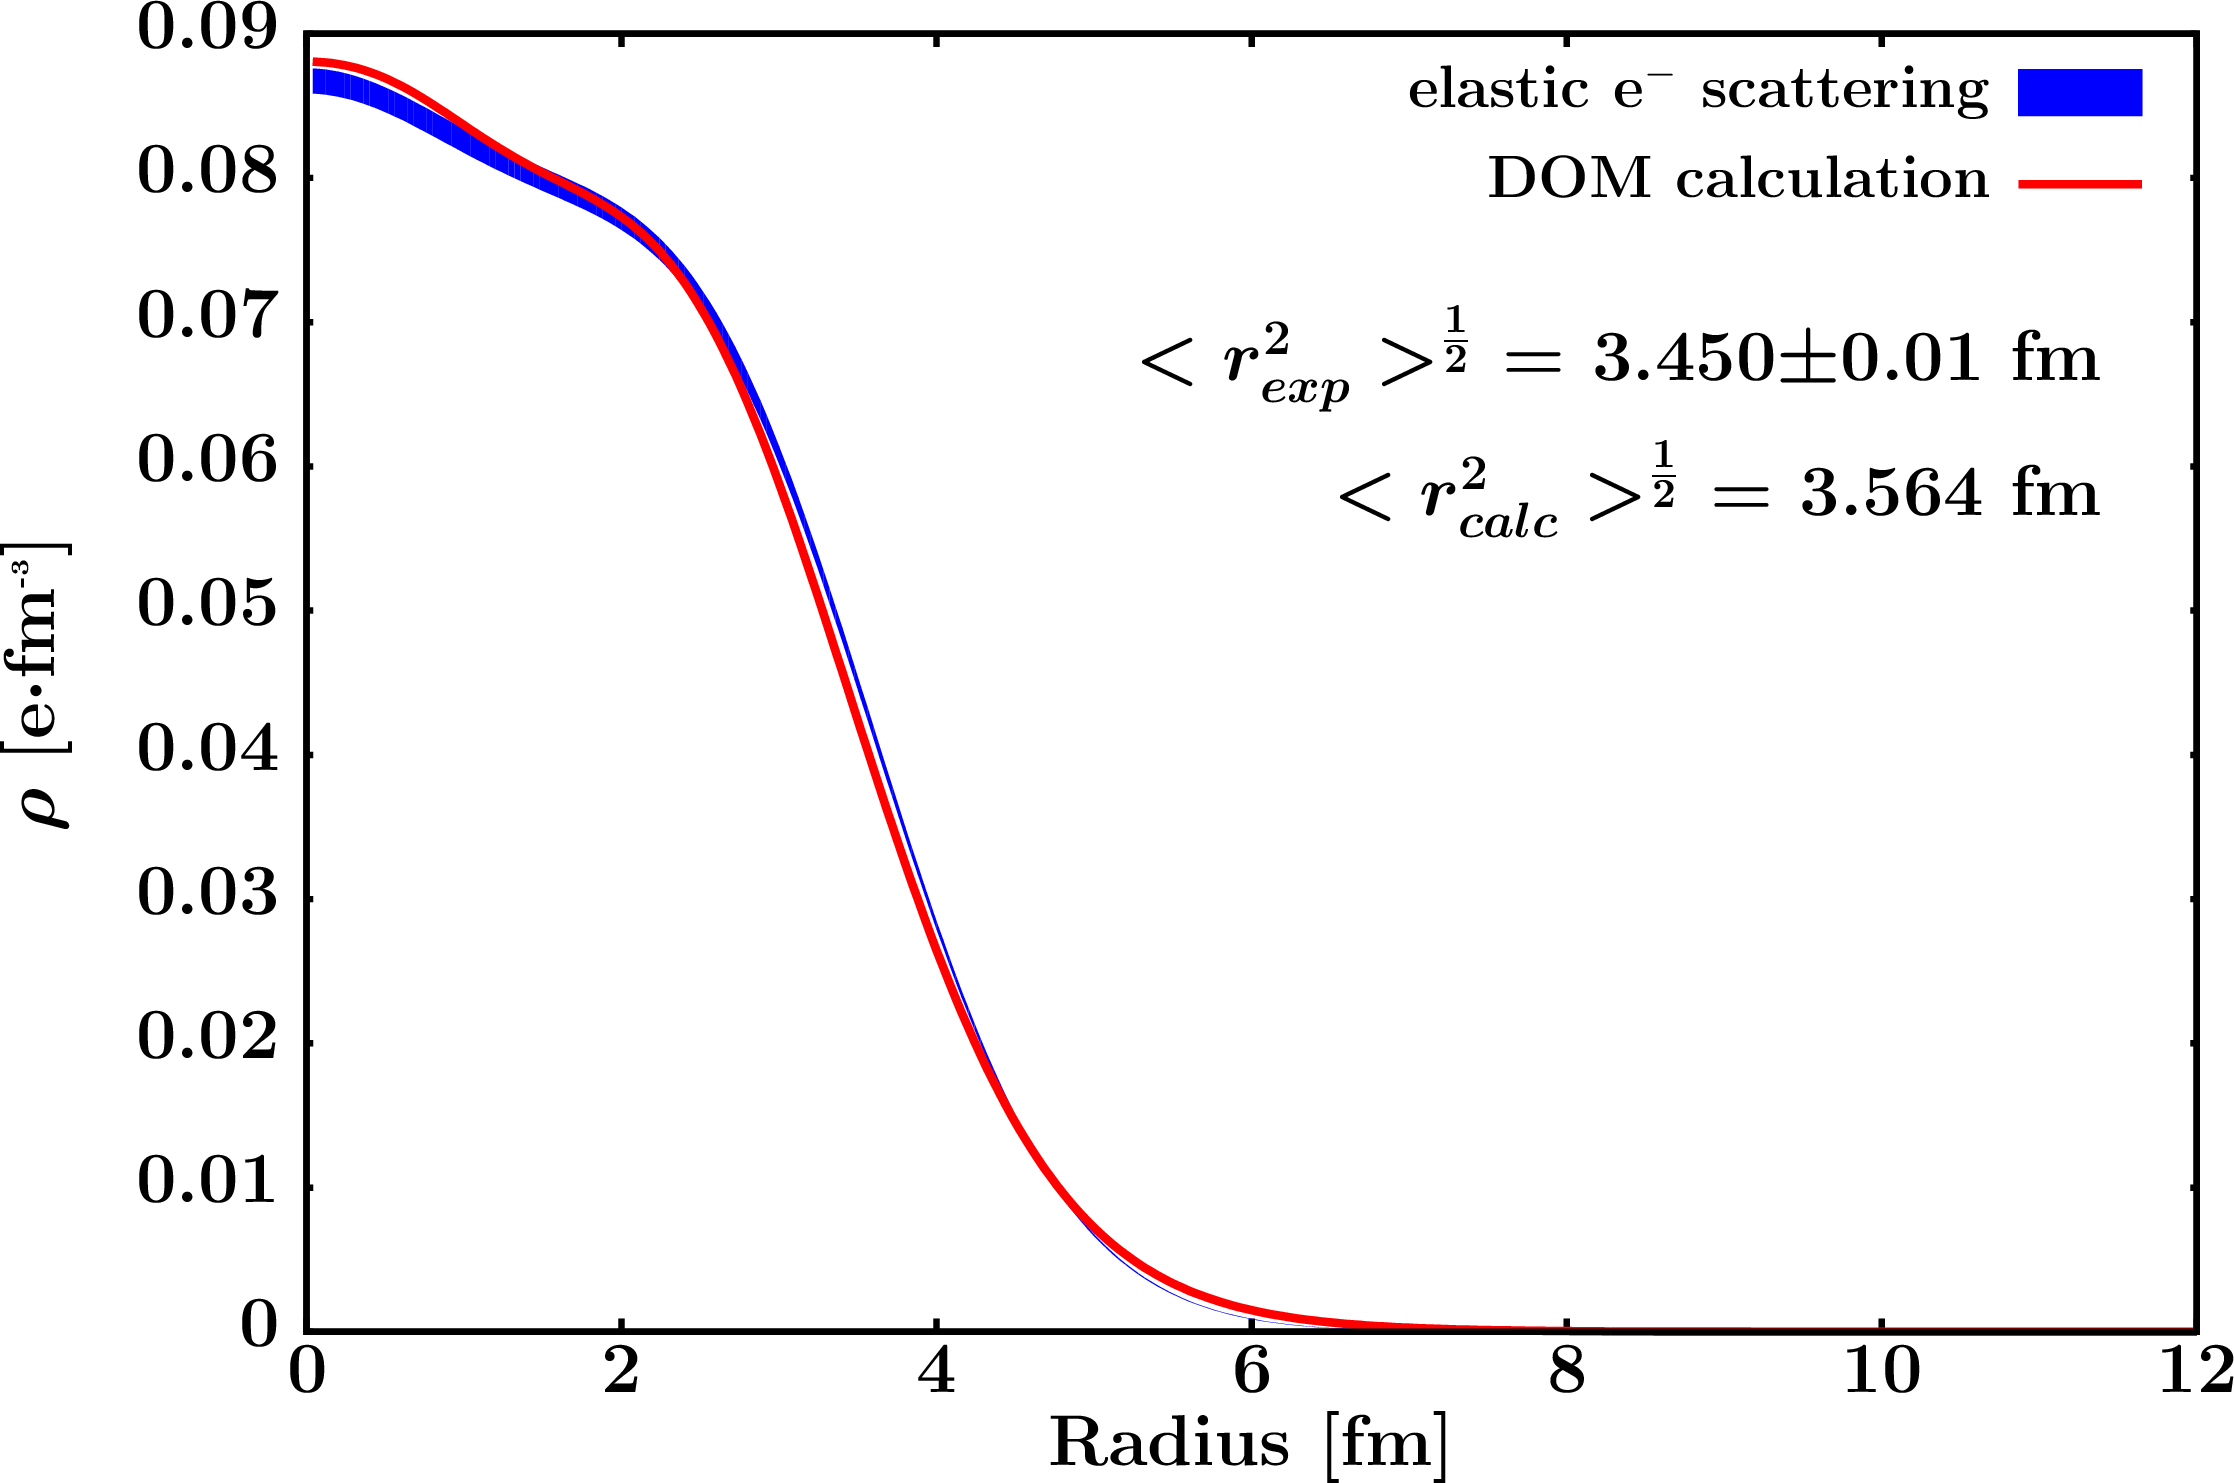
\includegraphics[width=\textwidth]{figures/ca40_chargeDensity.png}
        \caption*{\caForty\ charge density}
        \label{DOMFitData_ca40_chargeDensity}
    \end{minipage}\hspace{6pt}
    \begin{minipage}{0.42\textwidth}
        \centering
        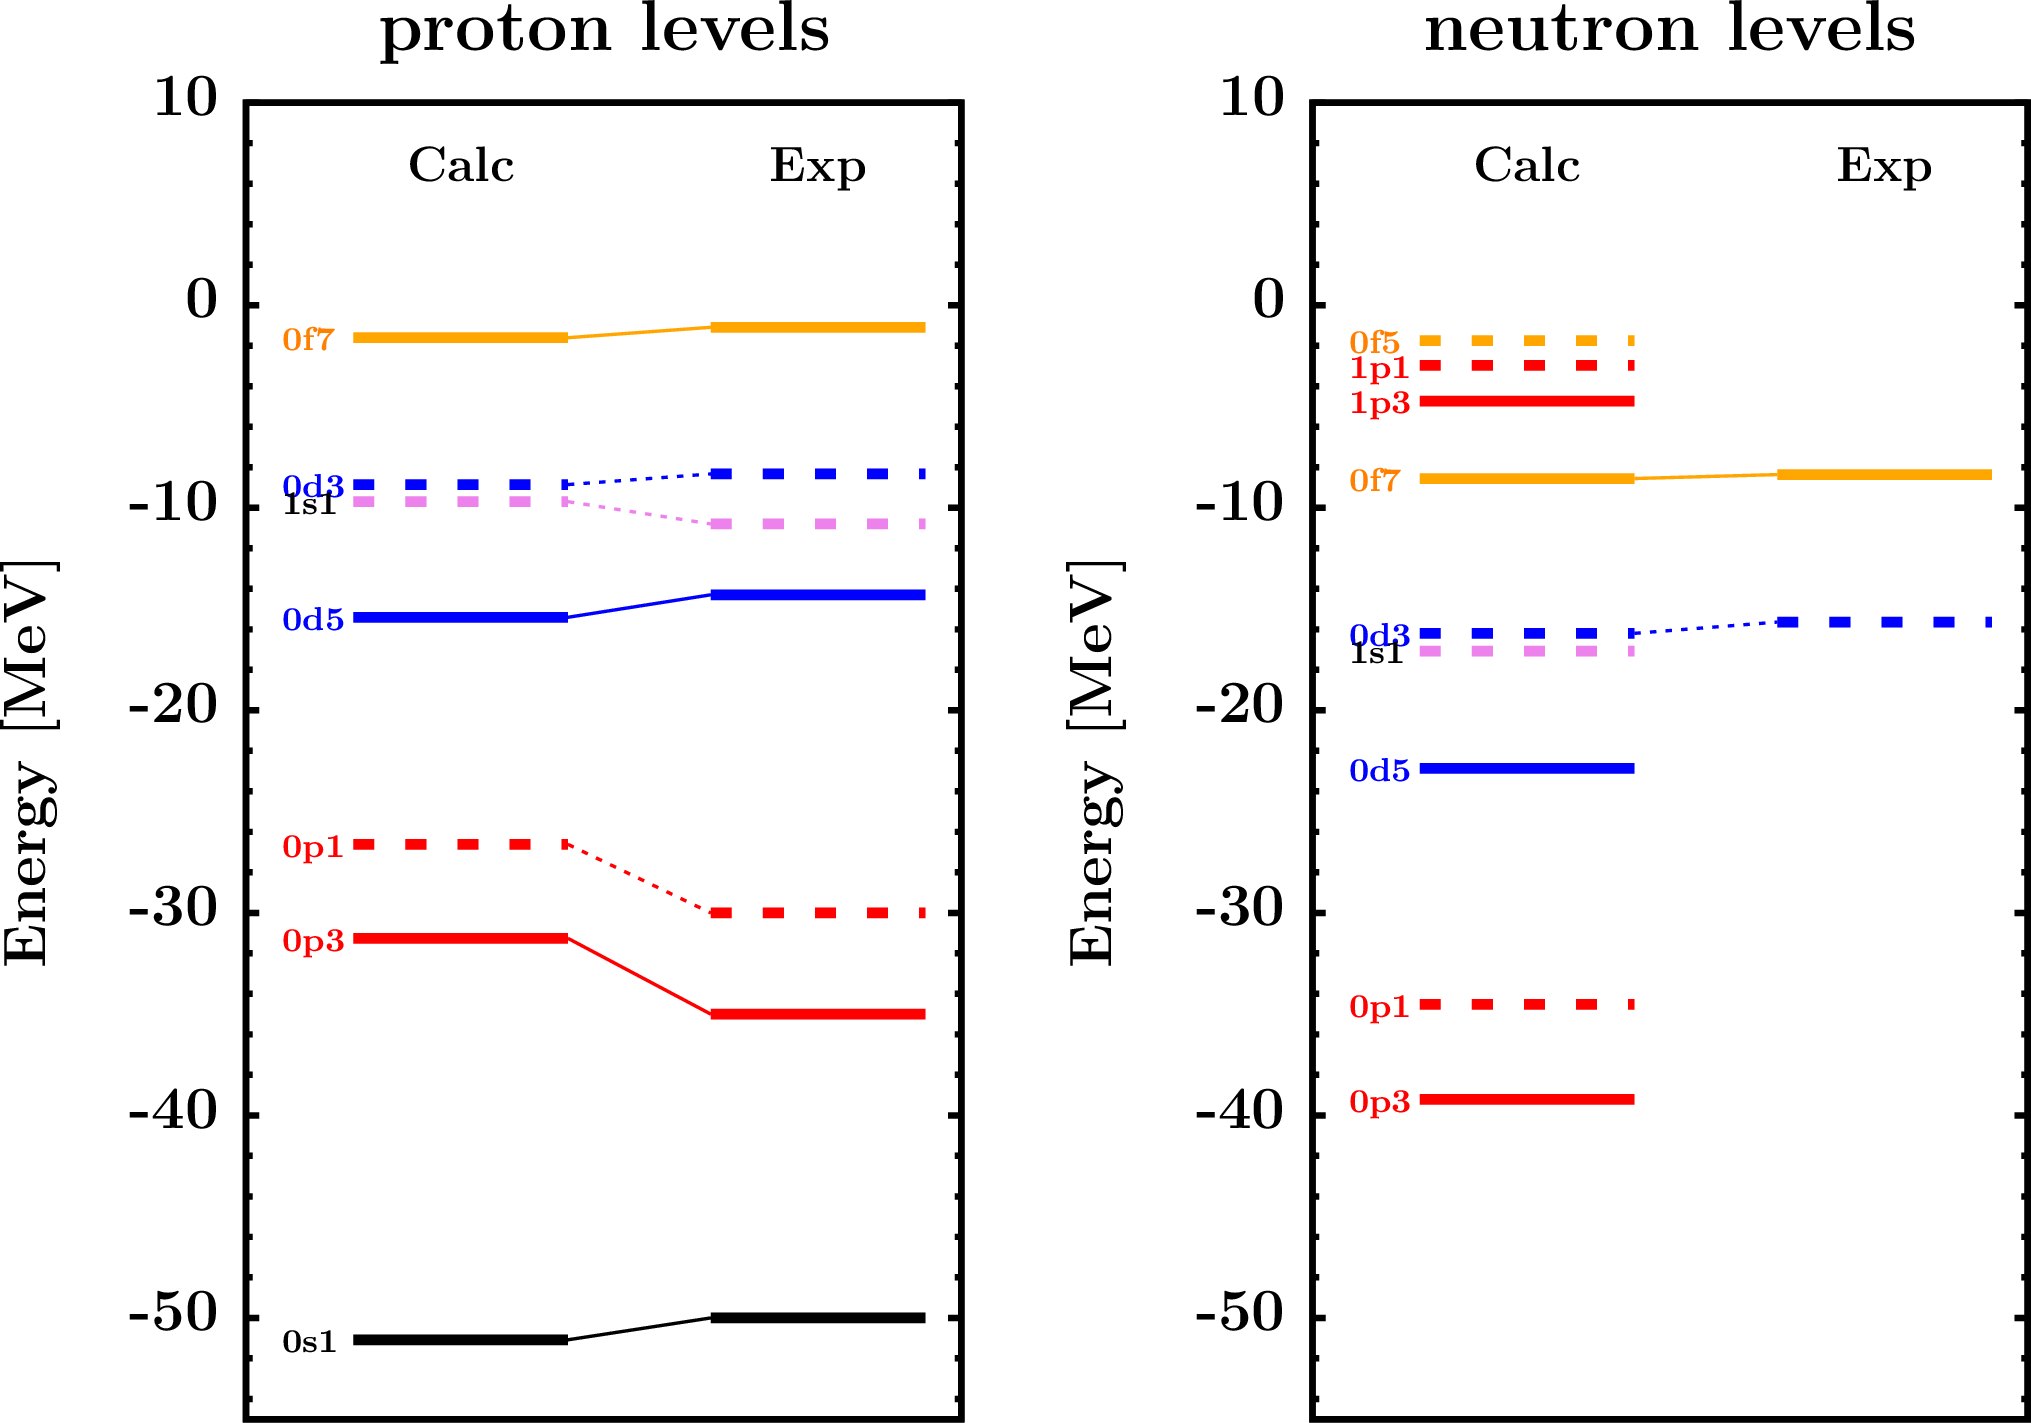
\includegraphics[width=\textwidth]{figures/ca40_SPLevels.png}
        \caption*{\caForty\ single-particle levels}
        \label{DOMFitData_ca40_SPLevels}
    \end{minipage}
\end{figure}
%\vspace{0.3in}
\begin{figure}[hbtp]
    \centering
    \begin{minipage}{0.42\textwidth}
        \centering
        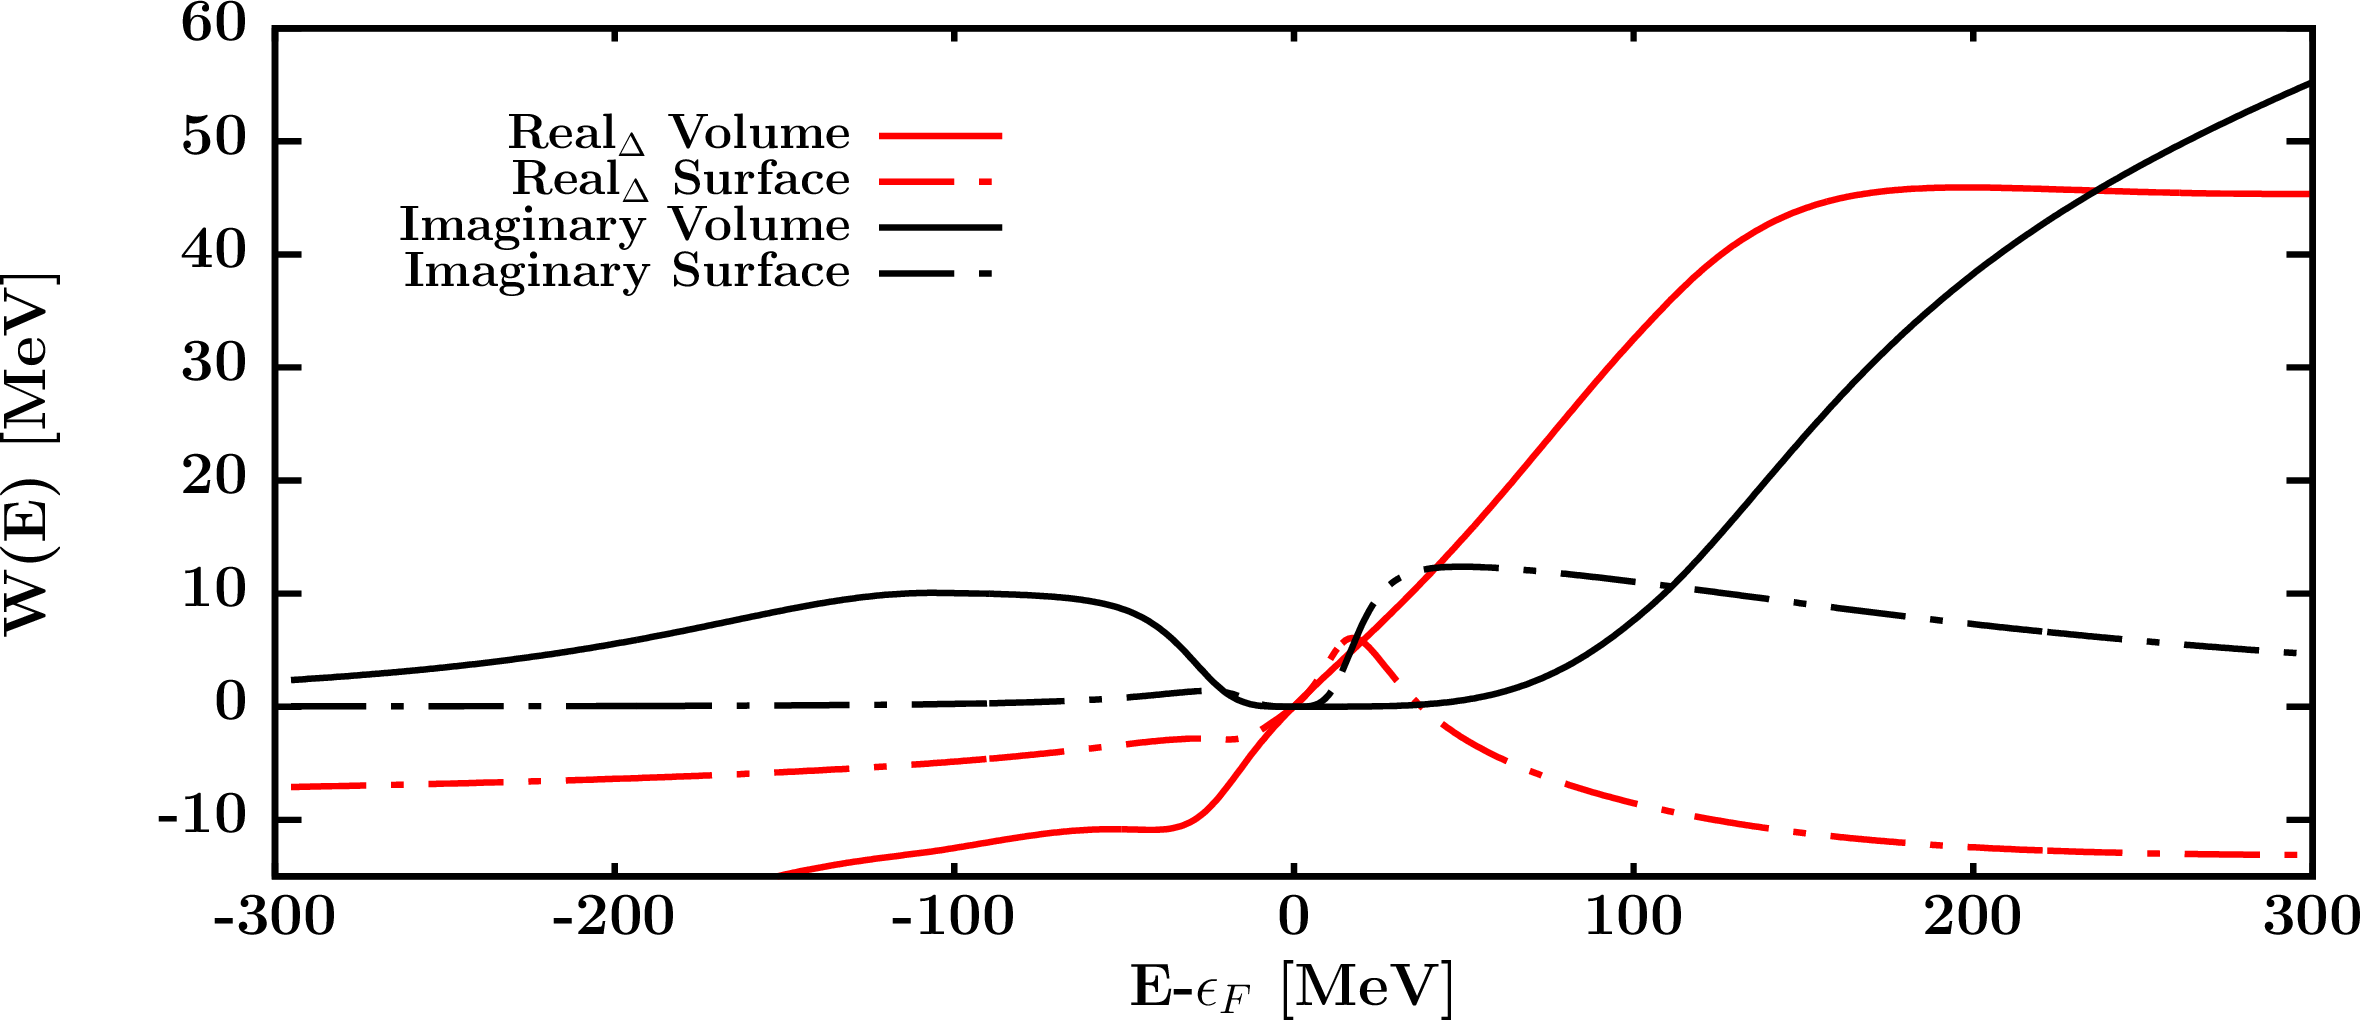
\includegraphics[width=\textwidth]{figures/ca40_protonPotentials.png}
        \caption*{\footnotesize\caForty\ proton potential energy dependence}
        \label{DOMFitData_ca40_proton_potentialComponent_energy}
    \end{minipage}\hspace{6pt}
    \begin{minipage}{0.42\textwidth}
        \centering
        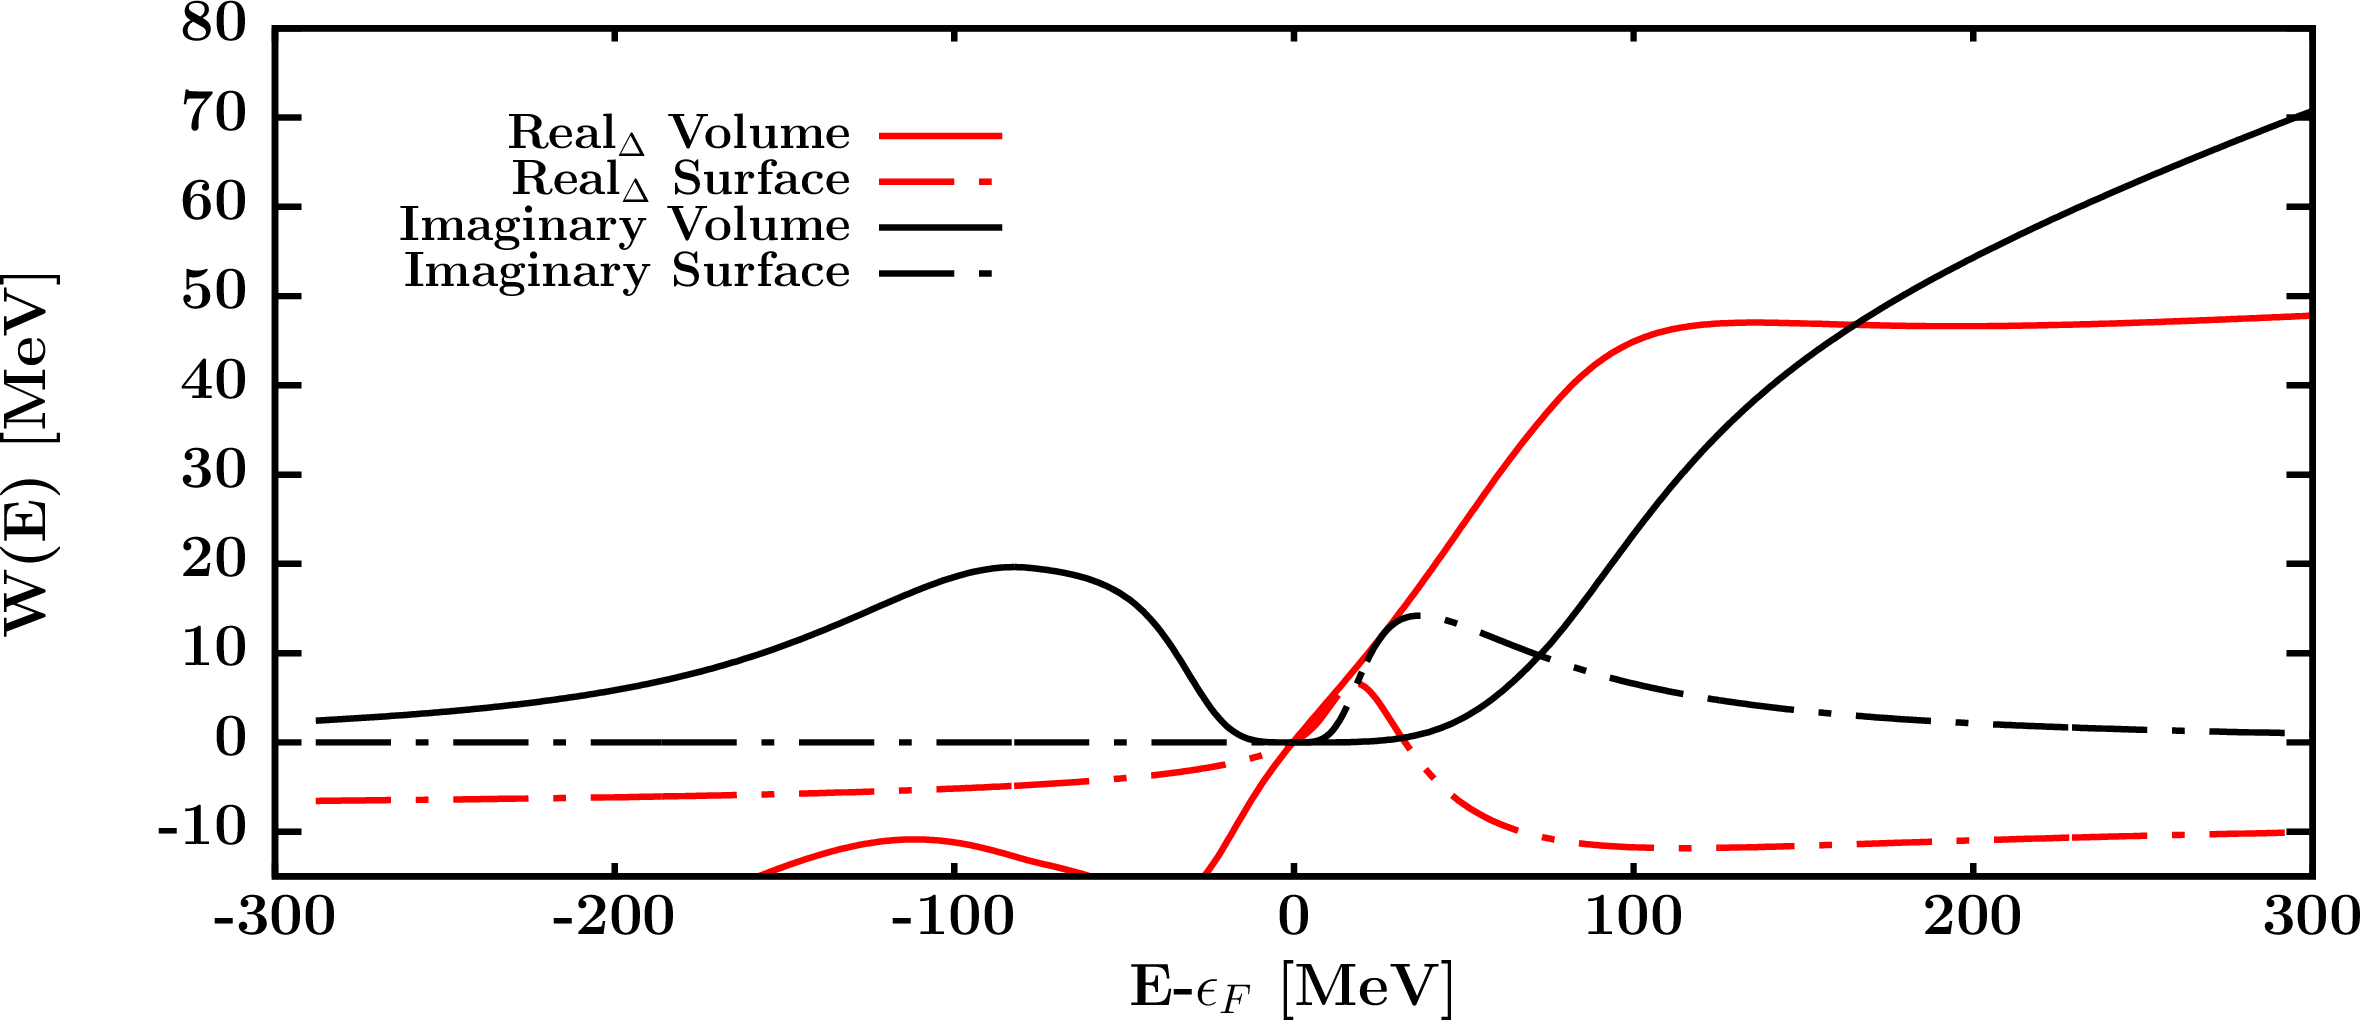
\includegraphics[width=\textwidth]{figures/ca40_neutronPotentials.png}
        \caption*{\footnotesize\caForty\ neutron potential energy dependence}
        \label{DOMFitData_ca40_neutron_potentialComponent_energy}
    \end{minipage}
\end{figure}
%\vspace{0.3in}
\begin{figure}[hbtp]
    \centering
    \begin{minipage}{0.42\textwidth}
        \centering
        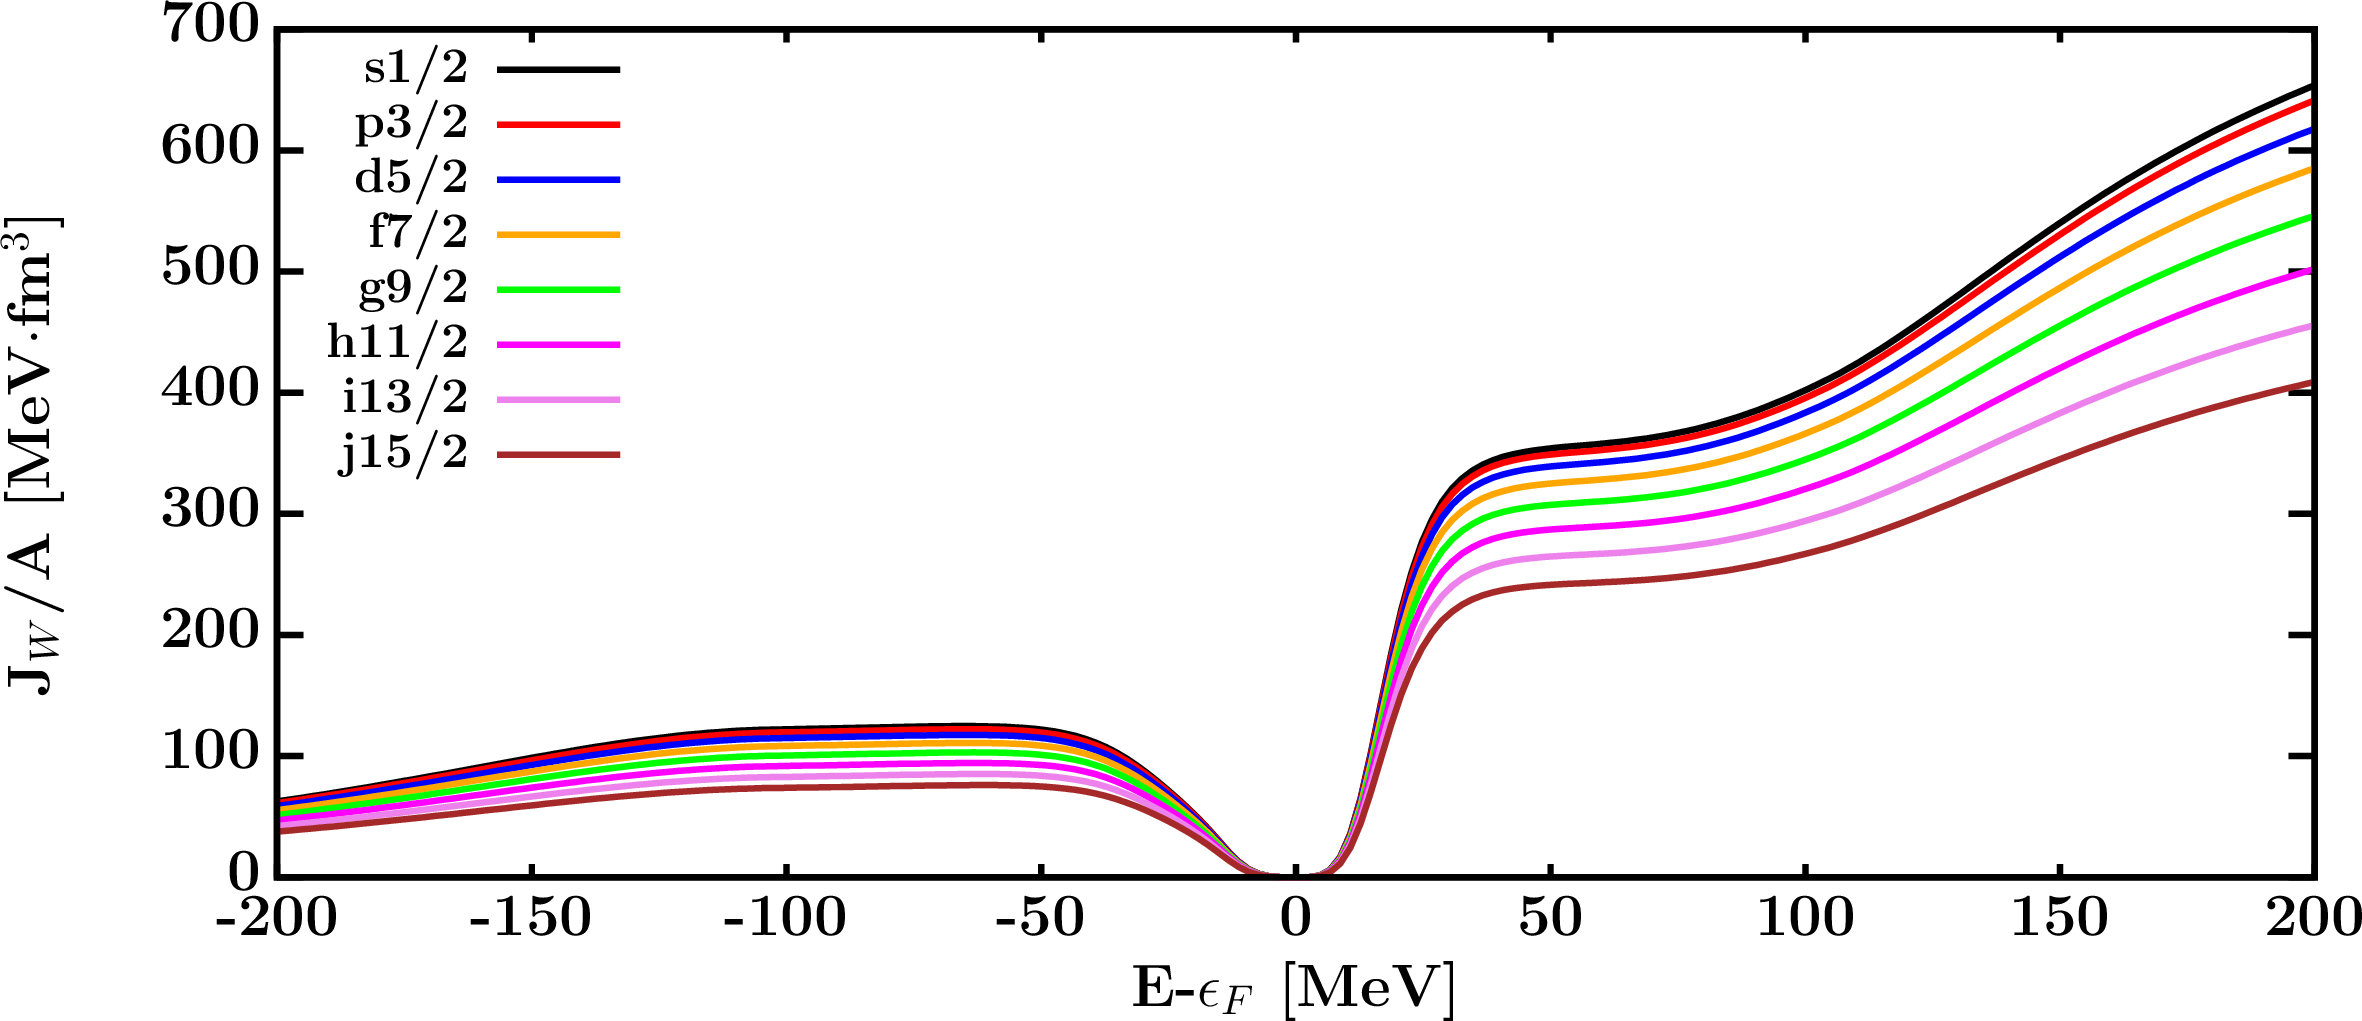
\includegraphics[width=\textwidth]{figures/ca40_protonVolumeIntegrals.png}
        \caption*{\caForty\ proton volume integral}
        \label{DOMFitData_ca40_proton_potentialIntegral}
    \end{minipage}\hspace{6pt}
    \begin{minipage}{0.42\textwidth}
        \centering
        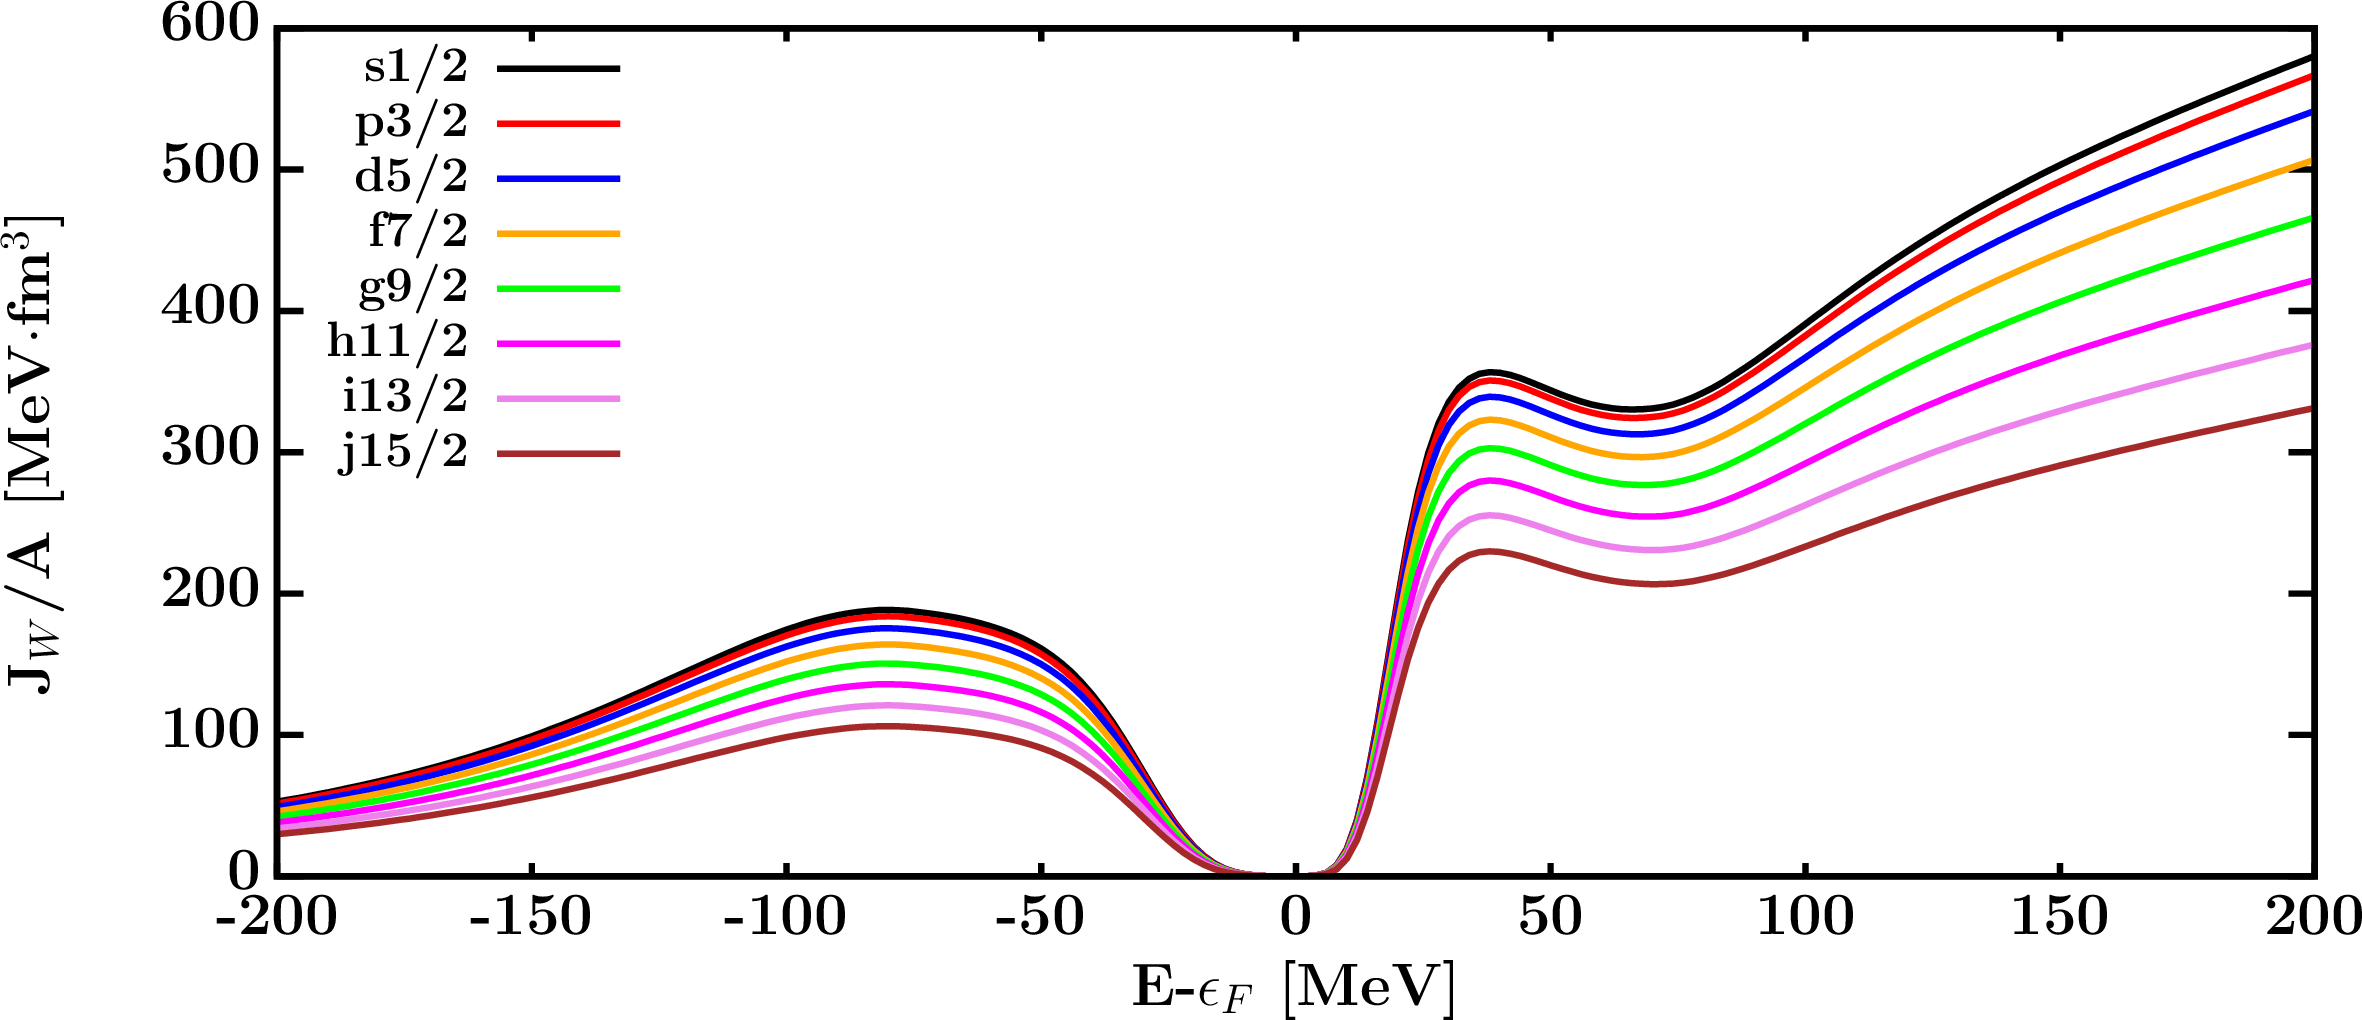
\includegraphics[width=\textwidth]{figures/ca40_neutronVolumeIntegrals.png}
        \caption*{\caForty\ neutron volume integral}
        \label{DOMFitData_ca40_neutron_potentialIntegral}
    \end{minipage}
\end{figure}
%\vspace{0.3in}
\begin{figure}[hbtp]
    \centering
    \begin{minipage}{0.42\textwidth}
        \centering
        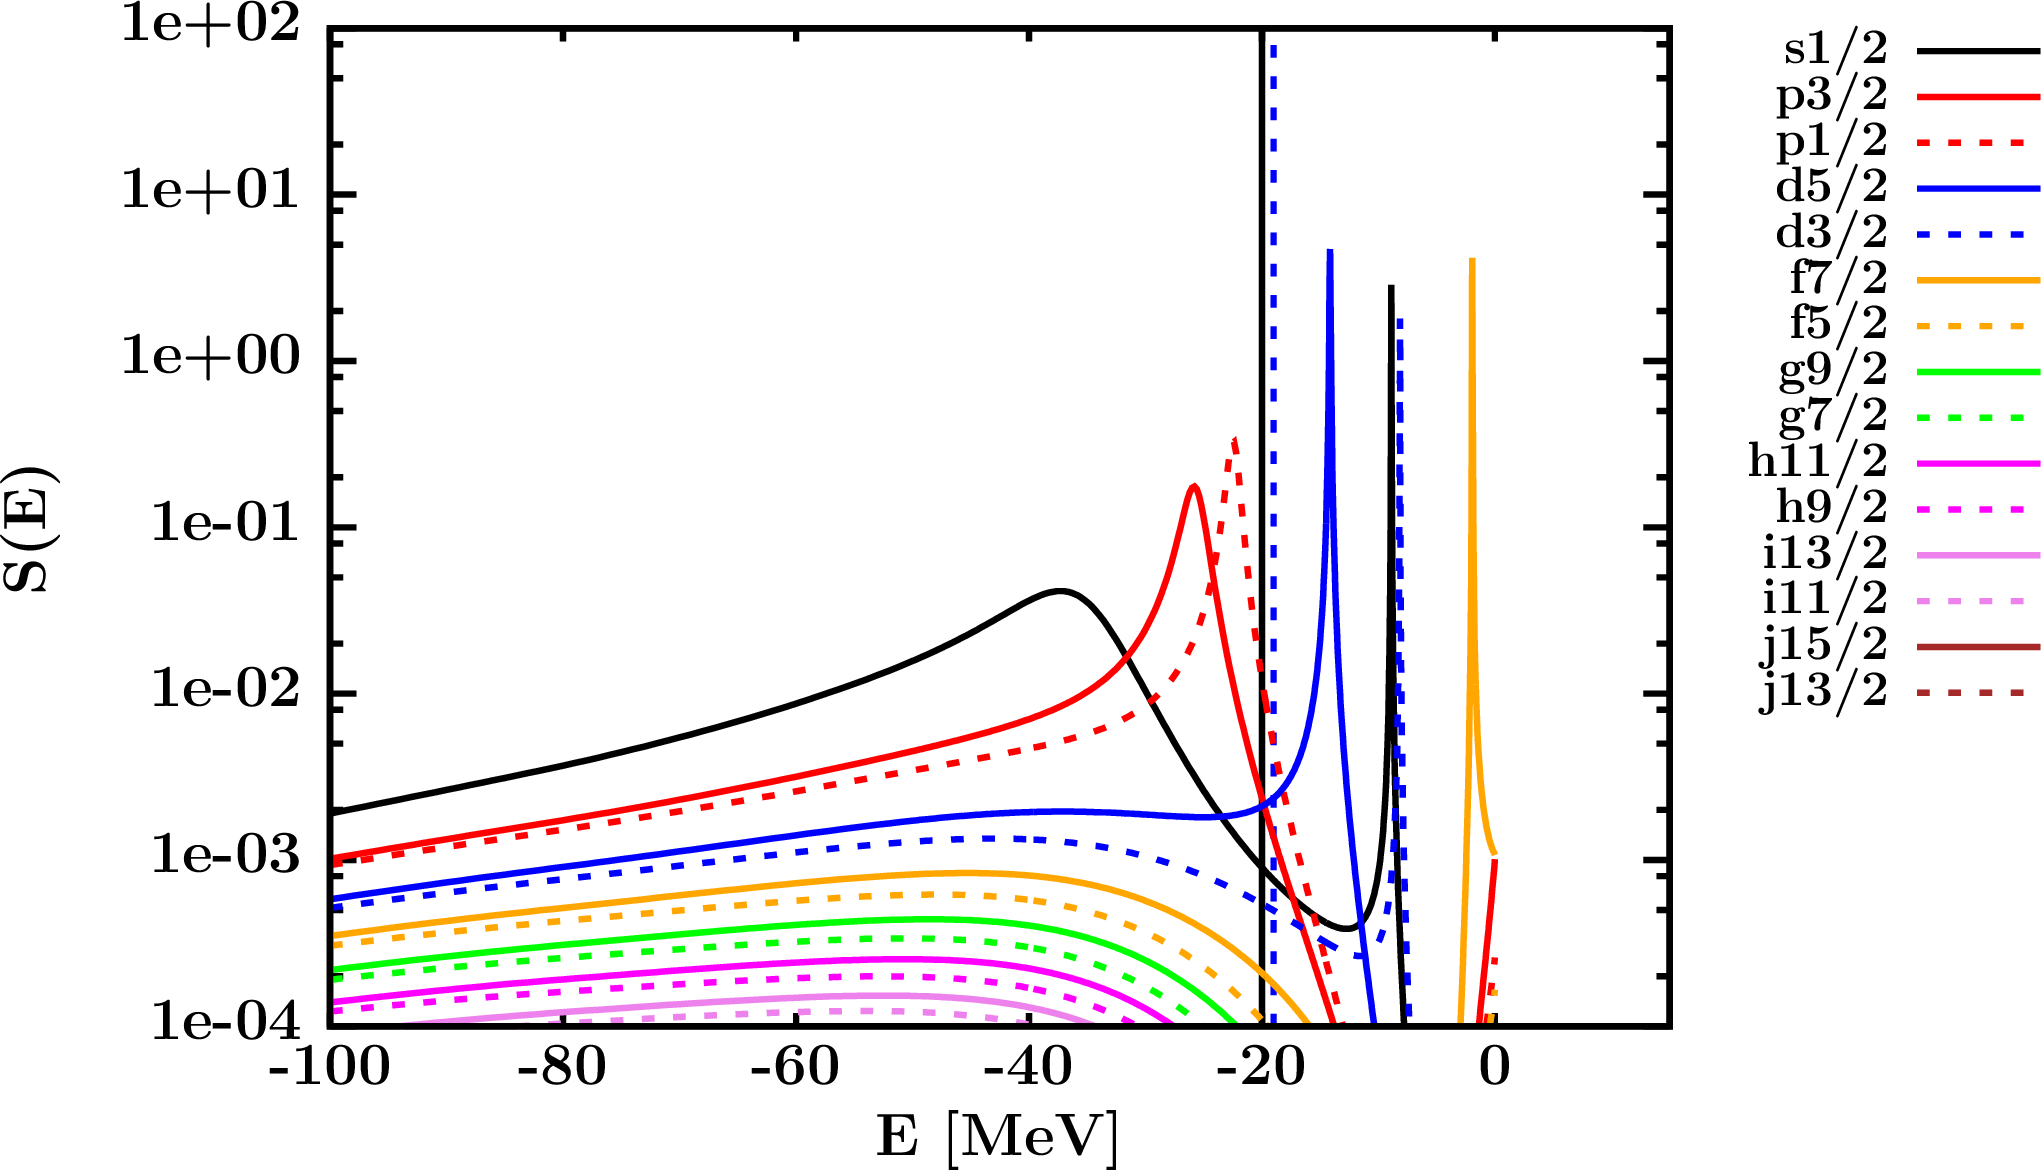
\includegraphics[width=\textwidth]{figures/ca40_protonSpectralFunctions.png}
        \caption*{\caForty\ proton spectral functions}
        \label{DOMFitData_ca40_proton_spectralFunctions}
    \end{minipage}\hspace{6pt}
    \begin{minipage}{0.42\textwidth}
        \centering
        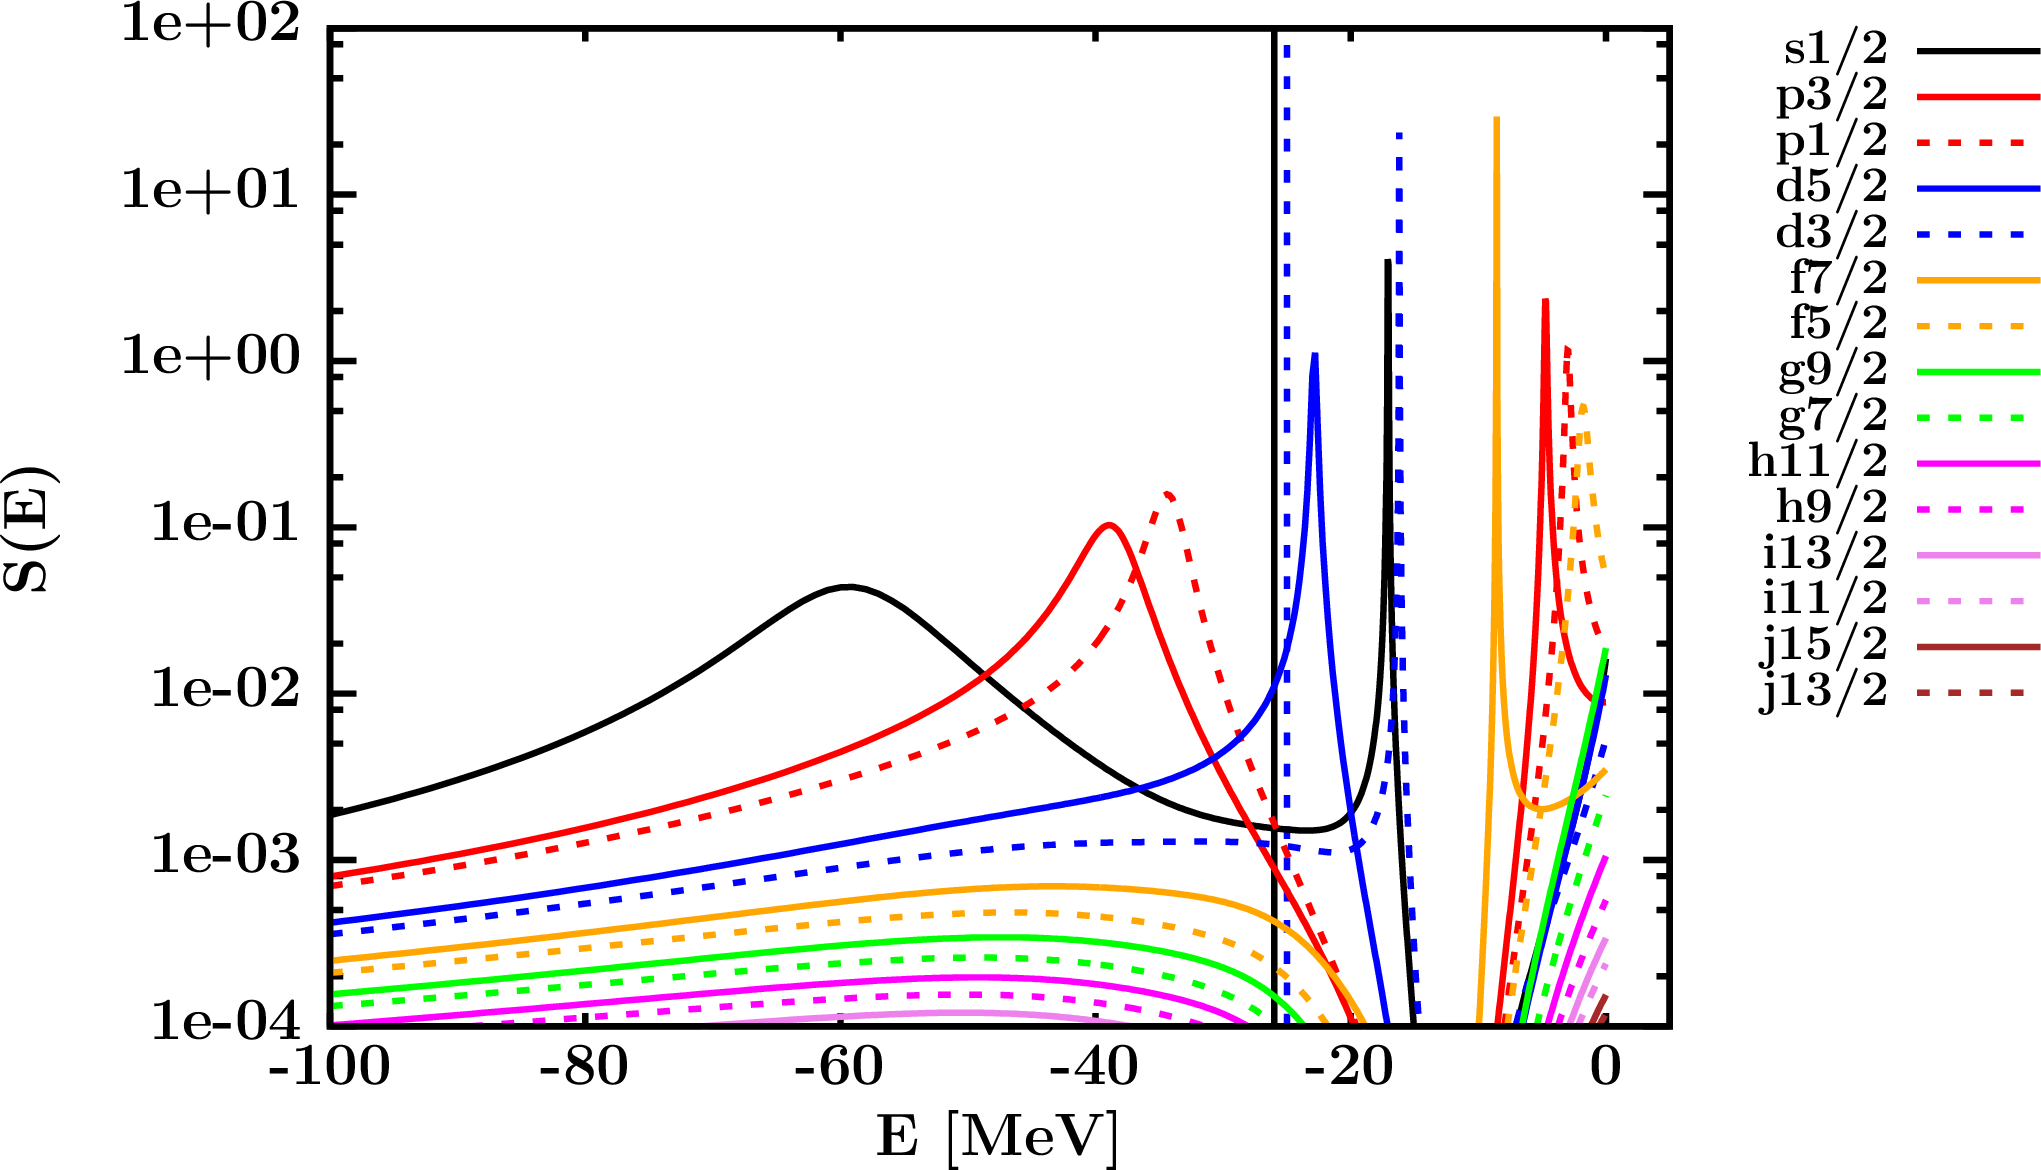
\includegraphics[width=\linewidth]{figures/ca40_neutronSpectralFunctions.png}
        \caption*{\caForty\ neutron spectral functions}
        \label{DOMFitData_ca40_neutron_spectralFunctions}
    \end{minipage}
\end{figure}
%\afterpage{\clearpage}
\begin{figure}[hbtp]
    \centering
    \begin{minipage}{0.45\textwidth}
        \centering
        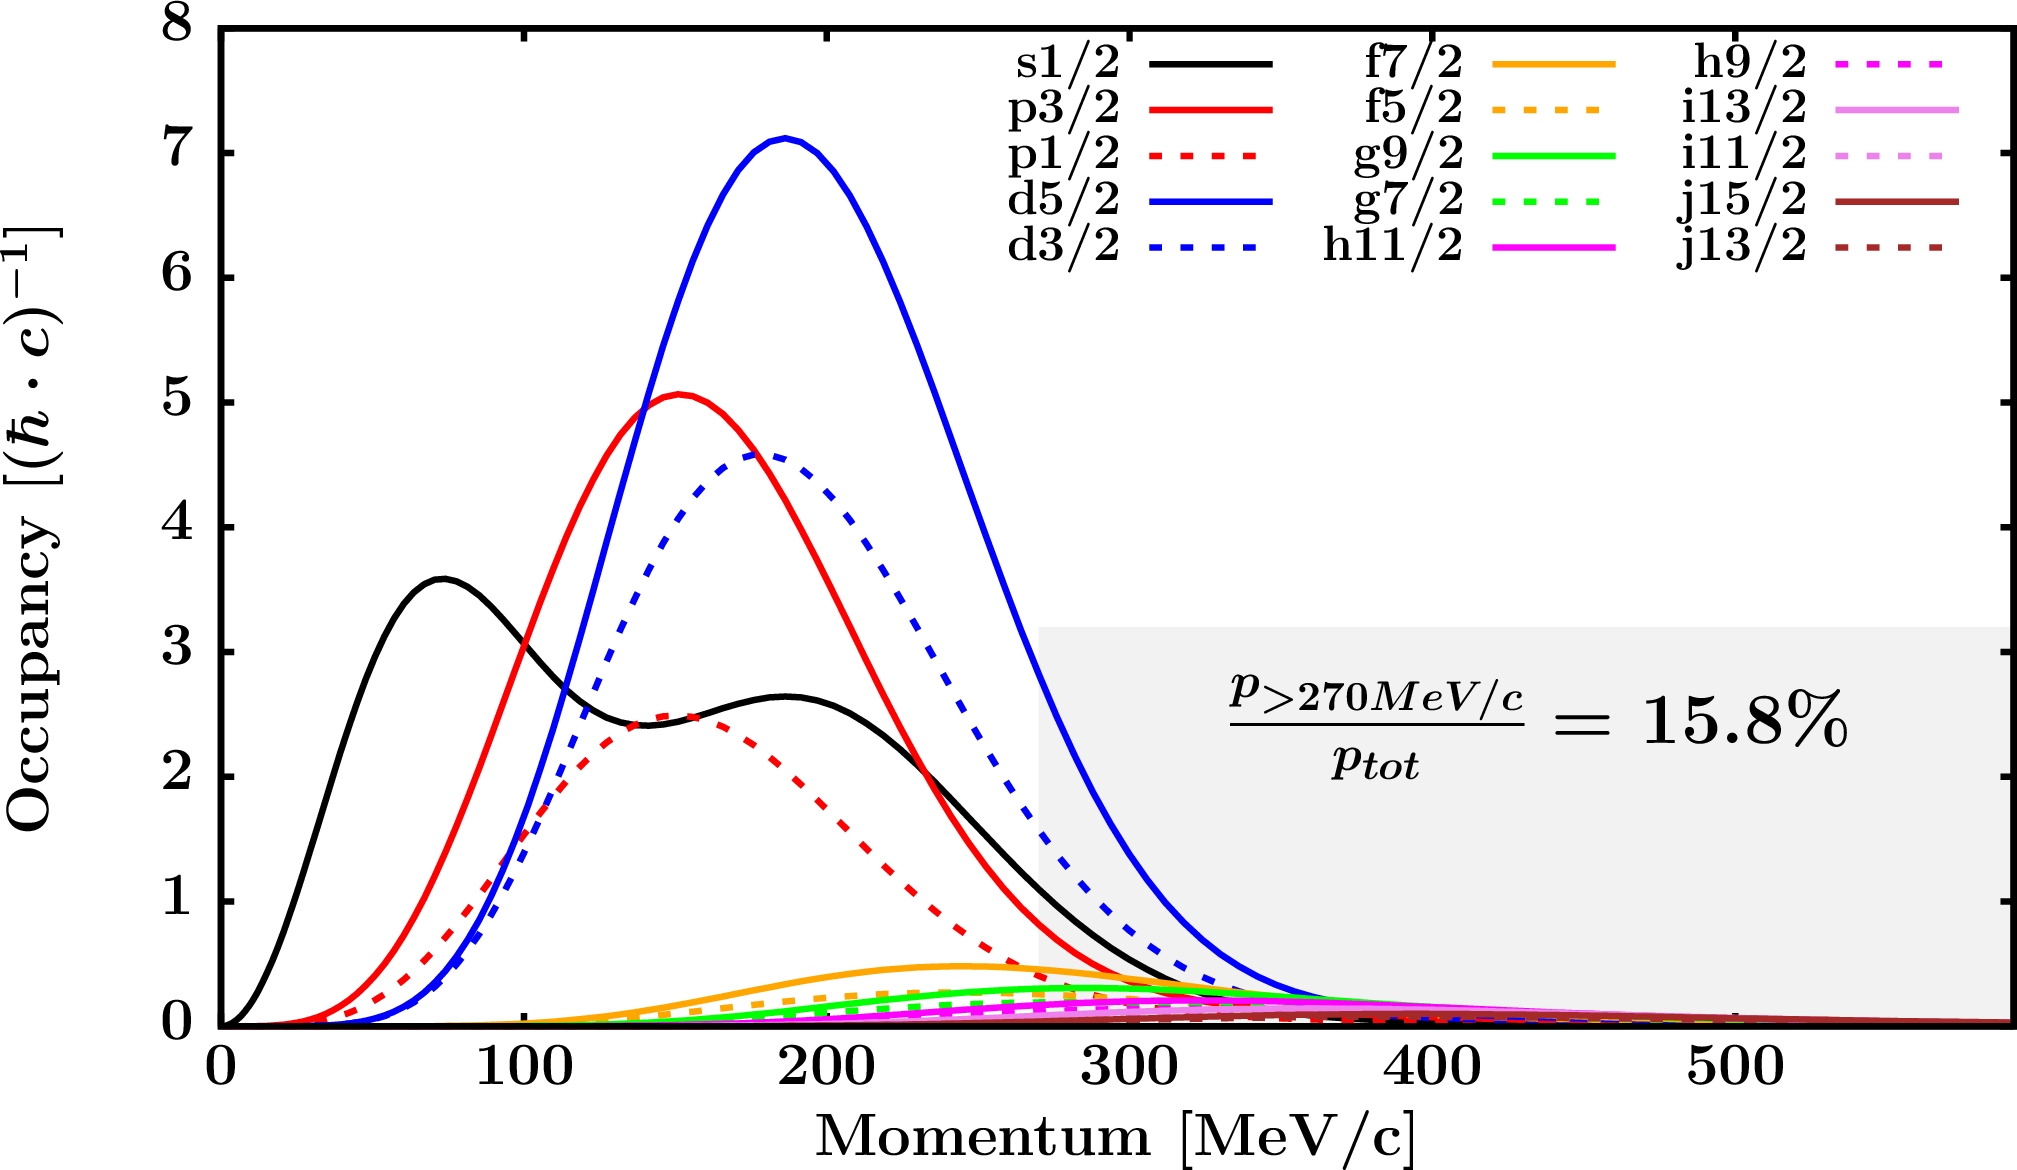
\includegraphics[width=\textwidth]{figures/ca40_protonLJMomentumDistIntegral.png}
        \caption*{\caForty\ proton momentum distribution}
        \label{DOMFitData_ca40_proton_momentumDist}
    \end{minipage}\hspace{6pt}
    \begin{minipage}{0.45\textwidth}
        \centering
        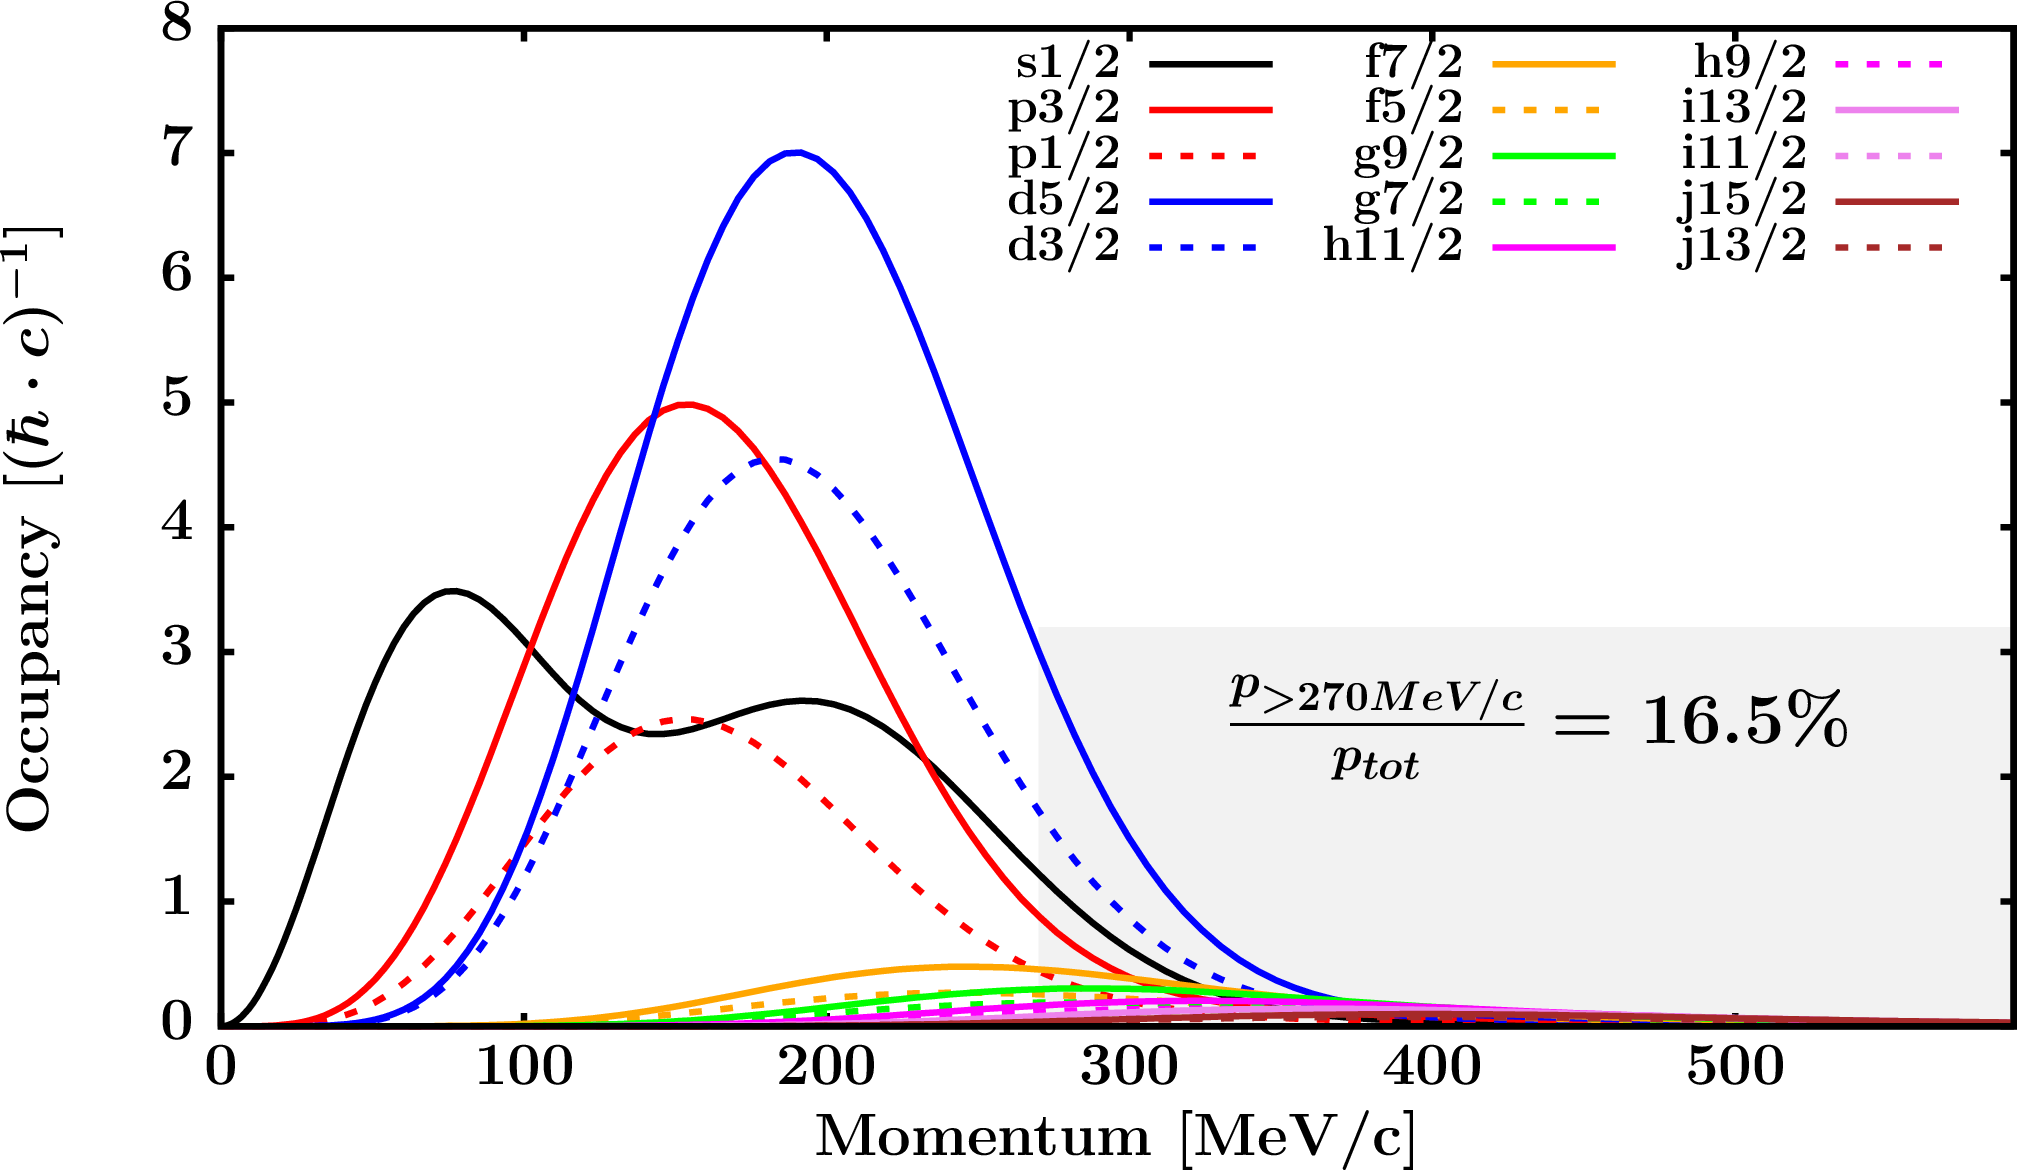
\includegraphics[width=\textwidth]{figures/ca40_neutronLJMomentumDistIntegral.png}
        \caption*{\caForty\ neutron momentum distribution}
        \label{DOMFitData_ca40_neutron_momentumDist}
    \end{minipage}
\end{figure}
\vspace{0.3in}
\begin{figure}[hbtp]
    \centering
    \begin{minipage}{0.45\textwidth}
        \centering
        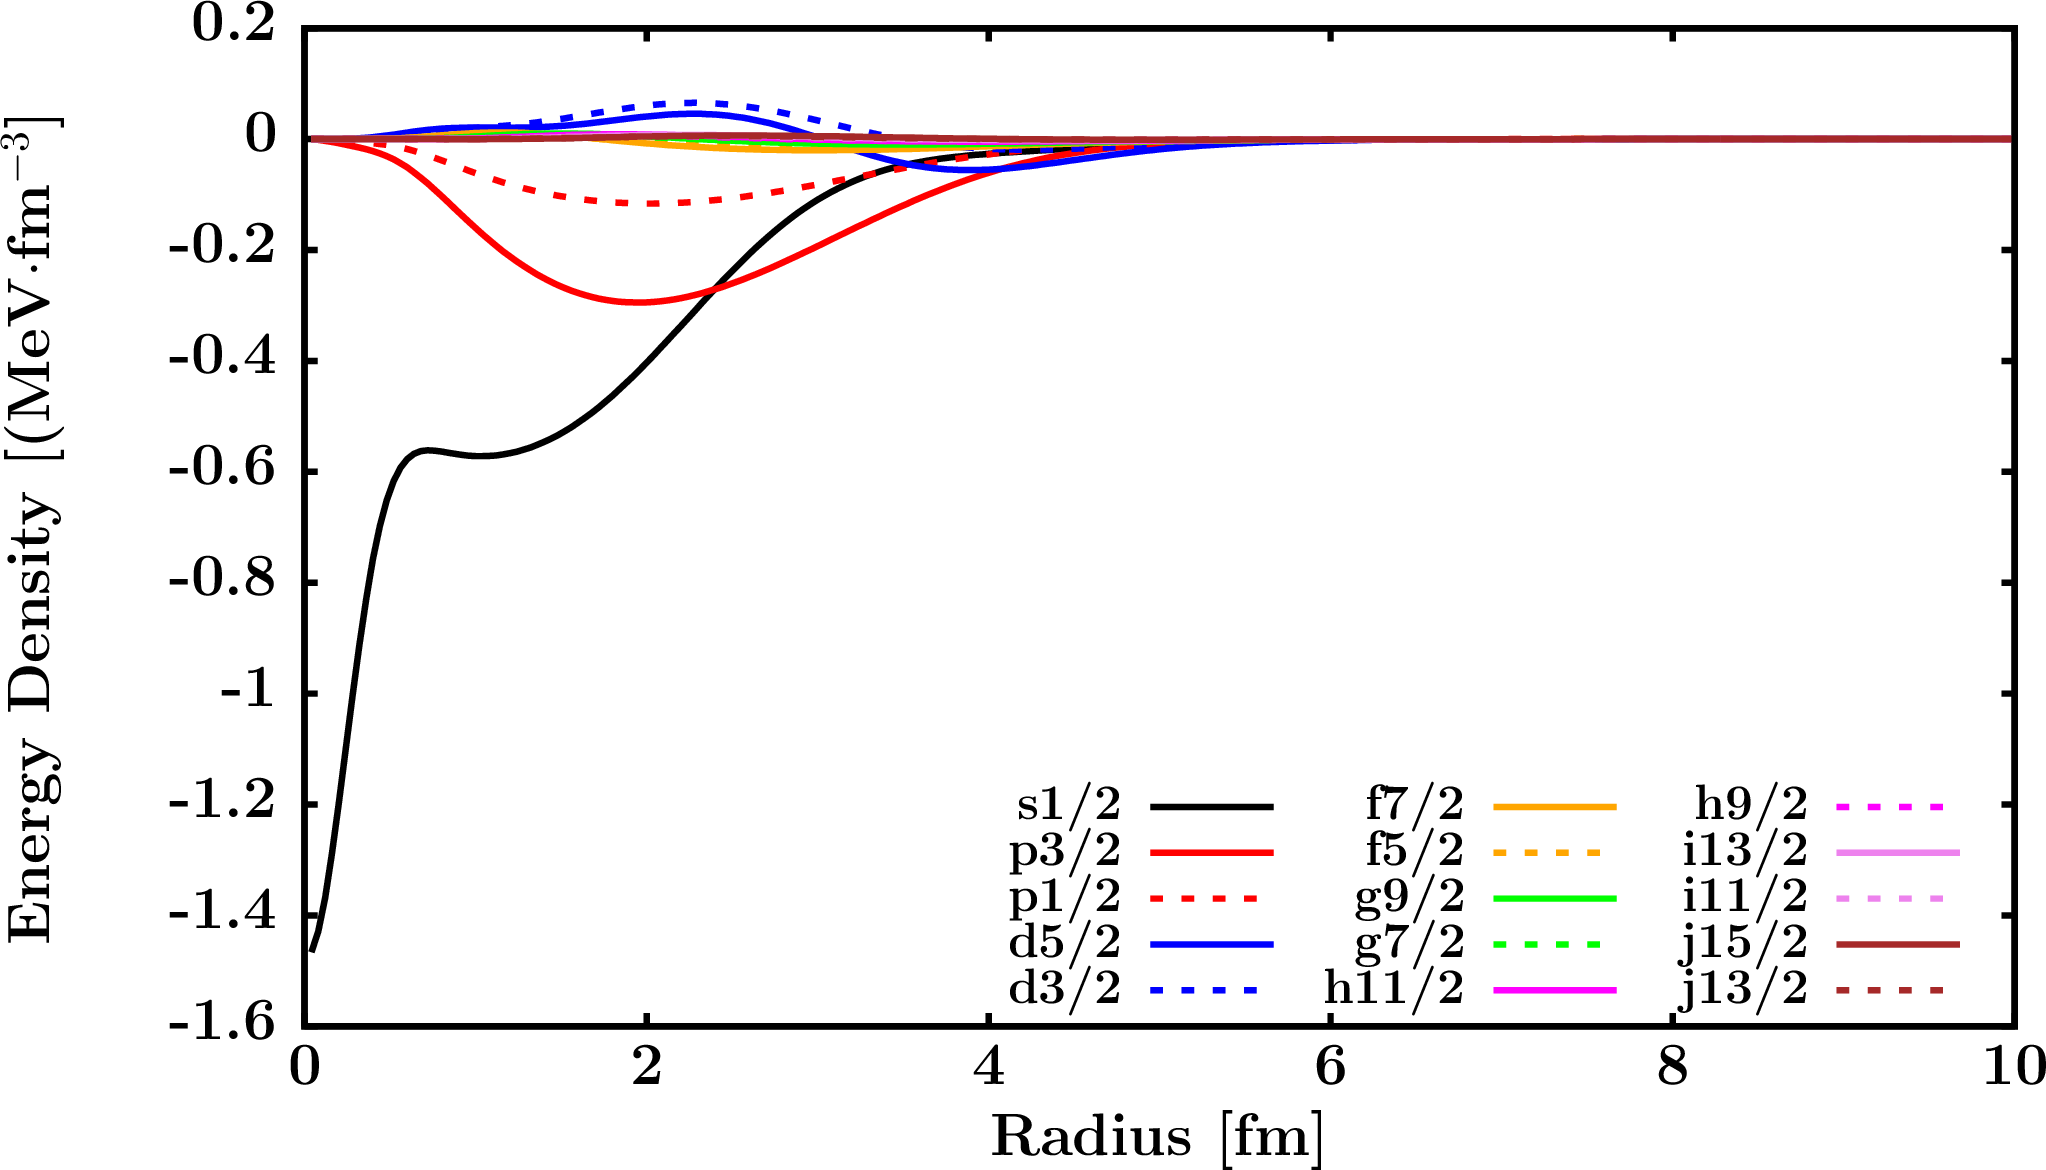
\includegraphics[width=\textwidth]{figures/ca40_EnergyDist.png}
        \caption*{\caForty\ energy distribution by LJ}
        \label{DOMFitData_ca40_proton_energyDistInt}
    \end{minipage}\hspace{6pt}
    \begin{minipage}{0.45\textwidth}
        \centering
        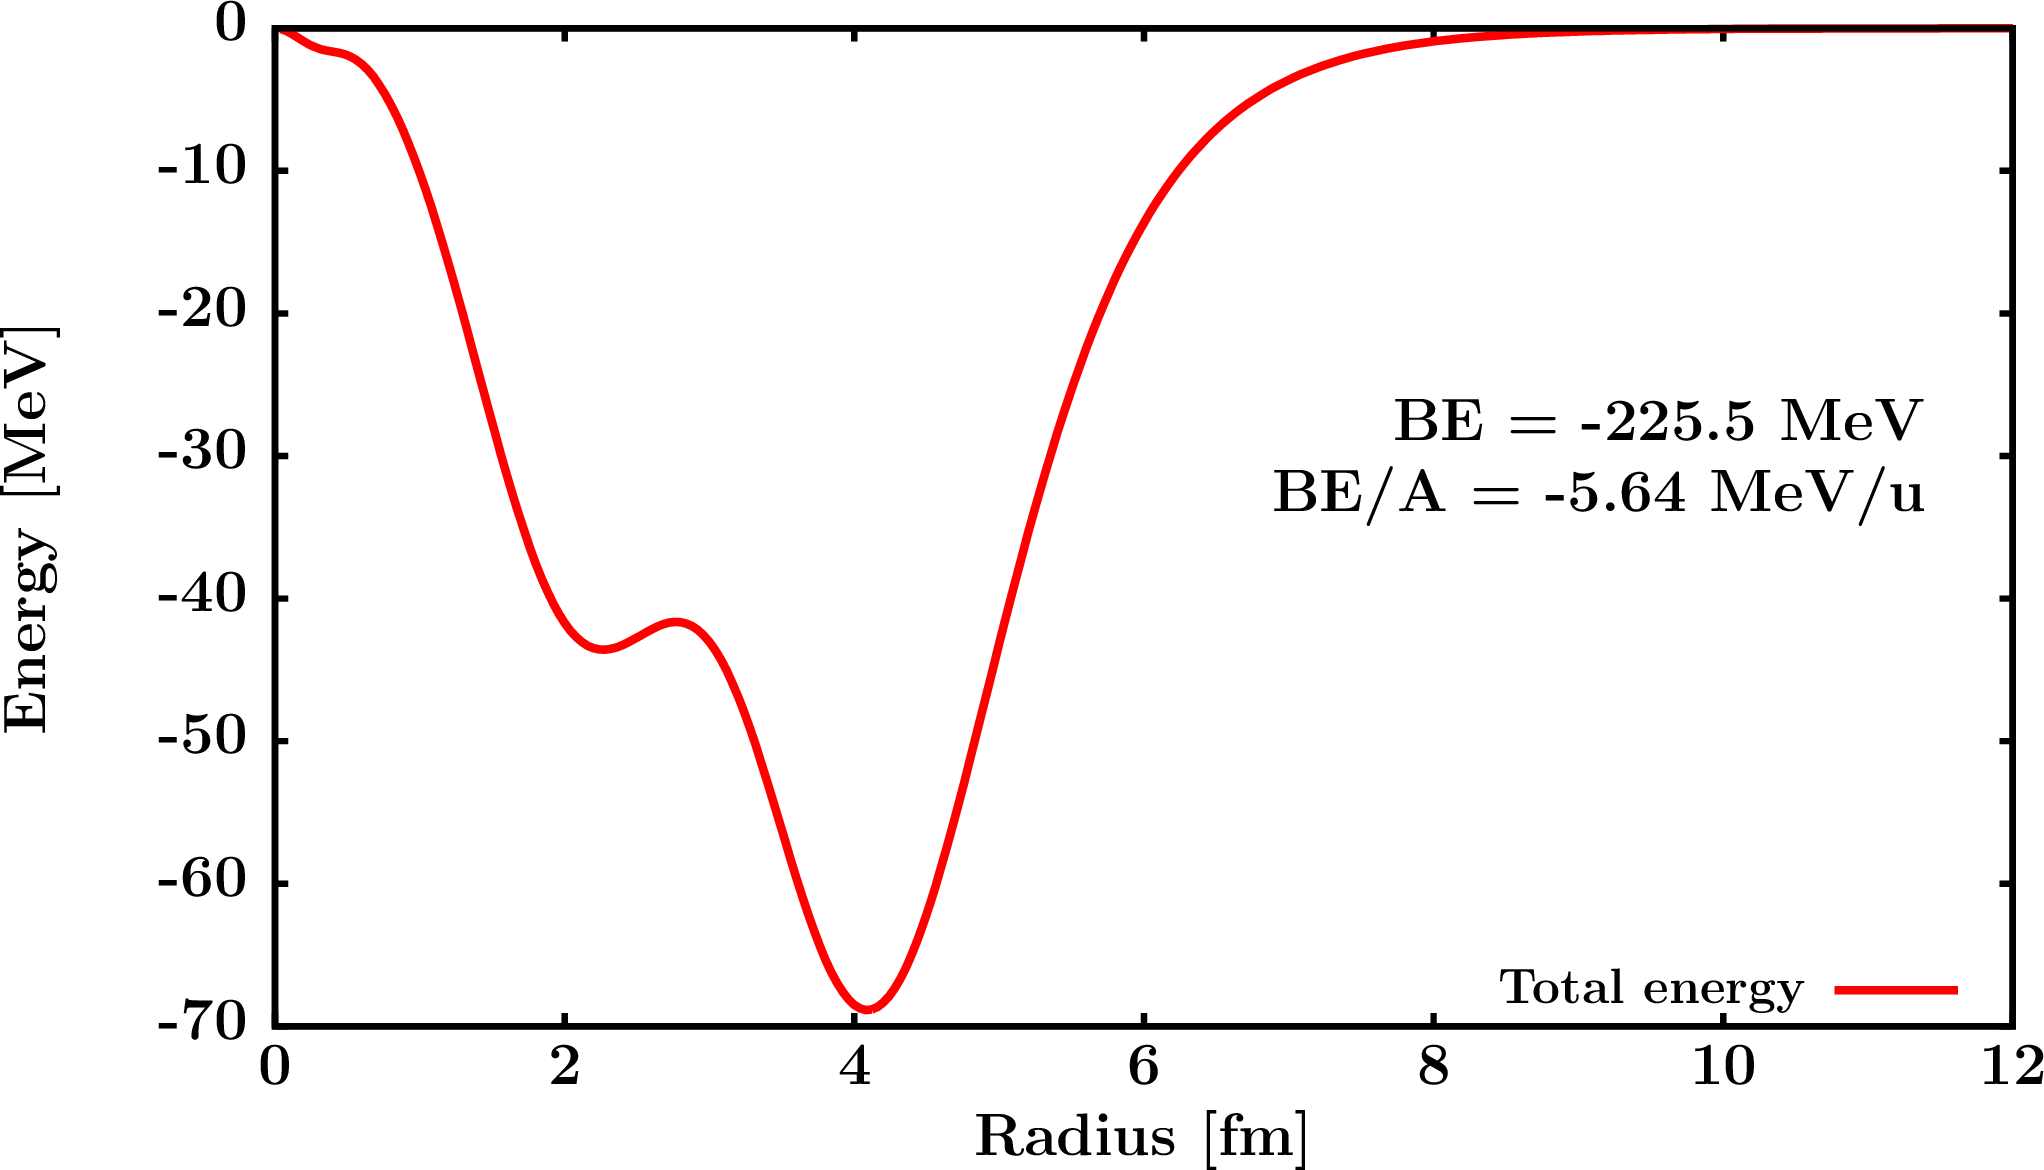
\includegraphics[width=\textwidth]{figures/ca40_EnergyDistIntegral.png}
        \caption*{\caForty\ energy distribution integral}
        \label{DOMFitData_ca40_neutron_energyDistInt}
    \end{minipage}
\end{figure}
\vspace{0.4in}
\begin{figure}[hbtp]
    \centering
    \begin{minipage}{0.70\textwidth}
        \centering
        \includegraphics[width=\linewidth]{figures/ca40_matterDensity.png}
        \caption*{\caForty\ matter density distribution}
        \label{DOMFitData_ca40_matterDensity}
    \end{minipage}
\end{figure}

\section{DOM fit of \caEight}
\label{ca48DOMOutput}
\begin{figure}[hbtp]
    \centering
    \begin{minipage}{0.47\textwidth}
        \centering
        \includegraphics[width=\textwidth]{figures/ca48_protonElastic.png}
        \caption*{\caEight\ proton elastic scattering}
        \label{DOMFitData_ca48_proton_elastic}
    \end{minipage}\hspace{6pt}
    \begin{minipage}{0.47\textwidth}
        \centering
        \includegraphics[width=0.52\textwidth]{figures/ca48_neutronElastic.png}
        \caption*{\caEight\ neutron elastic scattering}
        \label{DOMFitData_ca48_neutron_elastic}
    \end{minipage}
\end{figure}
\vspace{0.70in}
\begin{figure}[hbtp]
    \centering
    \begin{minipage}{0.47\textwidth}
        \centering
        \includegraphics[width=\linewidth]{figures/ca48_protonInelastic.png}
        \caption*{\caEight\ proton \rxn}
        \label{DOMFitData_ca48_proton_inelastic}
    \end{minipage}\hspace{6pt}
    \begin{minipage}{0.47\textwidth}
        \centering
        \includegraphics[width=\textwidth]{figures/ca48_neutronInelastic.png}
        \caption*{\caEight\ neutron \rxn\ and \tot}
        \label{DOMFitData_ca48_neutron_inelastic}
    \end{minipage}
\end{figure}
%\afterpage{\clearpage}
\begin{figure}[hbtp]
    \centering
    \begin{minipage}{0.42\textwidth}
        \centering
        \includegraphics[width=\textwidth]{figures/ca48_chargeDensity.png}
        \caption*{\caEight\ charge density}
        \label{DOMFitData_ca48_chargeDensity}
    \end{minipage}\hspace{6pt}
    \begin{minipage}{0.42\textwidth}
        \centering
        \includegraphics[width=\textwidth]{figures/ca48_SPLevels.png}
        \caption*{\caEight\ single-particle levels}
        \label{DOMFitData_ca48_SPLevels}
    \end{minipage}
\end{figure}
%\vspace{0.3in}
\begin{figure}[hbtp]
    \centering
    \begin{minipage}{0.42\textwidth}
        \centering
        \includegraphics[width=\textwidth]{figures/ca48_protonPotentials.png}
        \caption*{\footnotesize\caEight\ proton potential energy dependence}
        \label{DOMFitData_ca48_proton_potentialComponent_energy}
    \end{minipage}\hspace{6pt}
    \begin{minipage}{0.42\textwidth}
        \centering
        \includegraphics[width=\textwidth]{figures/ca48_neutronPotentials.png}
        \caption*{\footnotesize\caEight\ neutron potential energy dependence}
        \label{DOMFitData_ca48_neutron_potentialComponent_energy}
    \end{minipage}
\end{figure}
%\vspace{0.3in}
\begin{figure}[hbtp]
    \centering
    \begin{minipage}{0.42\textwidth}
        \centering
        \includegraphics[width=\textwidth]{figures/ca48_protonVolumeIntegrals.png}
        \caption*{\caEight\ proton volume integral}
        \label{DOMFitData_ca48_proton_potentialIntegral}
    \end{minipage}\hspace{6pt}
    \begin{minipage}{0.42\textwidth}
        \centering
        \includegraphics[width=\textwidth]{figures/ca48_neutronVolumeIntegrals.png}
        \caption*{\caEight\ neutron volume integral}
        \label{DOMFitData_ca48_neutron_potentialIntegral}
    \end{minipage}
\end{figure}
%\vspace{0.3in}
\begin{figure}[hbtp]
    \centering
    \begin{minipage}{0.42\textwidth}
        \centering
        \includegraphics[width=\textwidth]{figures/ca48_protonSpectralFunctions.png}
        \caption*{\caEight\ proton spectral functions}
        \label{DOMFitData_ca48_proton_spectralFunctions}
    \end{minipage}\hspace{6pt}
    \begin{minipage}{0.42\textwidth}
        \centering
        \includegraphics[width=\linewidth]{figures/ca48_neutronSpectralFunctions.png}
        \caption*{\caEight\ neutron spectral functions}
        \label{DOMFitData_ca48_neutron_spectralFunctions}
    \end{minipage}
\end{figure}
%\afterpage{\clearpage}
\begin{figure}[hbtp]
    \centering
    \begin{minipage}{0.45\textwidth}
        \centering
        \includegraphics[width=\textwidth]{figures/ca48_protonLJMomentumDistIntegral.png}
        \caption*{\caEight\ proton momentum distribution}
        \label{DOMFitData_ca48_proton_momentumDist}
    \end{minipage}\hspace{6pt}
    \begin{minipage}{0.45\textwidth}
        \centering
        \includegraphics[width=\textwidth]{figures/ca48_neutronLJMomentumDistIntegral.png}
        \caption*{\caEight\ neutron momentum distribution}
        \label{DOMFitData_ca48_neutron_momentumDist}
    \end{minipage}
\end{figure}
\vspace{0.3in}
\begin{figure}[hbtp]
    \centering
    \begin{minipage}{0.45\textwidth}
        \centering
        \includegraphics[width=\textwidth]{figures/ca48_EnergyDist.png}
        \caption*{\caEight\ energy distribution by LJ}
        \label{DOMFitData_ca48_proton_energyDistInt}
    \end{minipage}\hspace{6pt}
    \begin{minipage}{0.45\textwidth}
        \centering
        \includegraphics[width=\textwidth]{figures/ca48_EnergyDistIntegral.png}
        \caption*{\caEight\ energy distribution integral}
        \label{DOMFitData_ca48_neutron_energyDistInt}
    \end{minipage}
\end{figure}
\vspace{0.4in}
\begin{figure}[hbtp]
    \centering
    \begin{minipage}{0.70\textwidth}
        \centering
        \includegraphics[width=\linewidth]{figures/ca48_matterDensity.png}
        \caption*{\caEight\ matter density distribution}
        \label{DOMFitData_ca48_matterDensity}
    \end{minipage}
\end{figure}

\section{DOM fit of \niEight}
\label{ni58DOMOutput}
\begin{figure}[hbtp]
    \centering
    \begin{minipage}{0.47\textwidth}
        \centering
        \includegraphics[width=\textwidth]{figures/ni58_protonElastic.png}
        \caption*{\niEight\ proton elastic scattering}
        \label{DOMFitData_ni58_proton_elastic}
    \end{minipage}\hspace{6pt}
    \begin{minipage}{0.47\textwidth}
        \centering
        \includegraphics[width=\textwidth]{figures/ni58_neutronElastic.png}
        \caption*{\niEight\ neutron elastic scattering}
        \label{DOMFitData_ni58_neutron_elastic}
    \end{minipage}
\end{figure}
\vspace{0.70in}
\begin{figure}[hbtp]
    \centering
    \begin{minipage}{0.47\textwidth}
        \centering
        \includegraphics[width=\linewidth]{figures/ni58_protonInelastic.png}
        \caption*{\niEight\ proton \rxn}
        \label{DOMFitData_ni58_proton_inelastic}
    \end{minipage}\hspace{6pt}
    \begin{minipage}{0.47\textwidth}
        \centering
        \includegraphics[width=\textwidth]{figures/ni58_neutronInelastic.png}
        \caption*{\niEight\ neutron \rxn\ and \tot}
        \label{DOMFitData_ni58_neutron_inelastic}
    \end{minipage}
\end{figure}
%\afterpage{\clearpage}
\begin{figure}[hbtp]
    \centering
    \begin{minipage}{0.42\textwidth}
        \centering
        \includegraphics[width=\textwidth]{figures/ni58_chargeDensity.png}
        \caption*{\niEight\ charge density}
        \label{DOMFitData_ni58_chargeDensity}
    \end{minipage}\hspace{6pt}
    \begin{minipage}{0.42\textwidth}
        \centering
        \includegraphics[width=\textwidth]{figures/ni58_SPLevels.png}
        \caption*{\niEight\ single-particle levels}
        \label{DOMFitData_ni58_SPLevels}
    \end{minipage}
\end{figure}
%\vspace{0.3in}
\begin{figure}[hbtp]
    \centering
    \begin{minipage}{0.42\textwidth}
        \centering
        \includegraphics[width=\textwidth]{figures/ni58_protonPotentials.png}
        \caption*{\footnotesize\niEight\ proton potential energy dependence}
        \label{DOMFitData_ni58_proton_potentialComponent_energy}
    \end{minipage}\hspace{6pt}
    \begin{minipage}{0.42\textwidth}
        \centering
        \includegraphics[width=\textwidth]{figures/ni58_neutronPotentials.png}
        \caption*{\footnotesize\niEight\ neutron potential energy dependence}
        \label{DOMFitData_ni58_neutron_potentialComponent_energy}
    \end{minipage}
\end{figure}
%\vspace{0.3in}
\begin{figure}[hbtp]
    \centering
    \begin{minipage}{0.42\textwidth}
        \centering
        \includegraphics[width=\textwidth]{figures/ni58_protonVolumeIntegrals.png}
        \caption*{\niEight\ proton volume integral}
        \label{DOMFitData_ni58_proton_potentialIntegral}
    \end{minipage}\hspace{6pt}
    \begin{minipage}{0.42\textwidth}
        \centering
        \includegraphics[width=\textwidth]{figures/ni58_neutronVolumeIntegrals.png}
        \caption*{\niEight\ neutron volume integral}
        \label{DOMFitData_ni58_neutron_potentialIntegral}
    \end{minipage}
\end{figure}
%\vspace{0.3in}
\begin{figure}[hbtp]
    \centering
    \begin{minipage}{0.42\textwidth}
        \centering
        \includegraphics[width=\textwidth]{figures/ni58_protonSpectralFunctions.png}
        \caption*{\niEight\ proton spectral functions}
        \label{DOMFitData_ni58_proton_spectralFunctions}
    \end{minipage}\hspace{6pt}
    \begin{minipage}{0.42\textwidth}
        \centering
        \includegraphics[width=\linewidth]{figures/ni58_neutronSpectralFunctions.png}
        \caption*{\niEight\ neutron spectral functions}
        \label{DOMFitData_ni58_neutron_spectralFunctions}
    \end{minipage}
\end{figure}
%\afterpage{\clearpage}
\begin{figure}[hbtp]
    \centering
    \begin{minipage}{0.45\textwidth}
        \centering
        \includegraphics[width=\textwidth]{figures/ni58_protonLJMomentumDistIntegral.png}
        \caption*{\niEight\ proton momentum distribution}
        \label{DOMFitData_ni58_proton_momentumDist}
    \end{minipage}\hspace{6pt}
    \begin{minipage}{0.45\textwidth}
        \centering
        \includegraphics[width=\textwidth]{figures/ni58_neutronLJMomentumDistIntegral.png}
        \caption*{\niEight\ neutron momentum distribution}
        \label{DOMFitData_ni58_neutron_momentumDist}
    \end{minipage}
\end{figure}
\vspace{0.3in}
\begin{figure}[hbtp]
    \centering
    \begin{minipage}{0.45\textwidth}
        \centering
        \includegraphics[width=\textwidth]{figures/ni58_EnergyDist.png}
        \caption*{\niEight\ energy distribution by LJ}
        \label{DOMFitData_ni58_proton_energyDistInt}
    \end{minipage}\hspace{6pt}
    \begin{minipage}{0.45\textwidth}
        \centering
        \includegraphics[width=\textwidth]{figures/ni58_EnergyDistIntegral.png}
        \caption*{\niEight\ energy distribution integral}
        \label{DOMFitData_ni58_neutron_energyDistInt}
    \end{minipage}
\end{figure}
\vspace{0.4in}
\begin{figure}[hbtp]
    \centering
    \begin{minipage}{0.70\textwidth}
        \centering
        \includegraphics[width=\linewidth]{figures/ni58_matterDensity.png}
        \caption*{\niEight\ matter density distribution}
        \label{DOMFitData_ni58_matterDensity}
    \end{minipage}
\end{figure}

\section{DOM fit of \niFour}
\label{ni64DOMOutput}
\begin{figure}[hbtp]
    \centering
    \begin{minipage}{0.47\textwidth}
        \centering
        \includegraphics[width=\textwidth]{figures/ni64_protonElastic.png}
        \caption*{\niFour\ proton elastic scattering}
        \label{DOMFitData_ni64_proton_elastic}
    \end{minipage}\hspace{6pt}
    \begin{minipage}{0.47\textwidth}
        \centering
        \includegraphics[width=0.52\textwidth]{figures/ni64_neutronElastic.png}
        \caption*{\niFour\ neutron elastic scattering}
        \label{DOMFitData_ni64_neutron_elastic}
    \end{minipage}
\end{figure}
\vspace{0.70in}
\begin{figure}[hbtp]
    \centering
    \begin{minipage}{0.47\textwidth}
        \centering
        \includegraphics[width=\linewidth]{figures/ni64_protonInelastic.png}
        \caption*{\niFour\ proton \rxn}
        \label{DOMFitData_ni64_proton_inelastic}
    \end{minipage}\hspace{6pt}
    \begin{minipage}{0.47\textwidth}
        \centering
        \includegraphics[width=\textwidth]{figures/ni64_neutronInelastic.png}
        \caption*{\niFour\ neutron \rxn\ and \tot}
        \label{DOMFitData_ni64_neutron_inelastic}
    \end{minipage}
\end{figure}
%\afterpage{\clearpage}
\begin{figure}[hbtp]
    \centering
    \begin{minipage}{0.42\textwidth}
        \centering
        \includegraphics[width=\textwidth]{figures/ni64_chargeDensity.png}
        \caption*{\niFour\ charge density}
        \label{DOMFitData_ni64_chargeDensity}
    \end{minipage}\hspace{6pt}
    \begin{minipage}{0.42\textwidth}
        \centering
        \includegraphics[width=\textwidth]{figures/ni64_SPLevels.png}
        \caption*{\niFour\ single-particle levels}
        \label{DOMFitData_ni64_SPLevels}
    \end{minipage}
\end{figure}
%\vspace{0.3in}
\begin{figure}[hbtp]
    \centering
    \begin{minipage}{0.42\textwidth}
        \centering
        \includegraphics[width=\textwidth]{figures/ni64_protonPotentials.png}
        \caption*{\footnotesize\niFour\ proton potential energy dependence}
        \label{DOMFitData_ni64_proton_potentialComponent_energy}
    \end{minipage}\hspace{6pt}
    \begin{minipage}{0.42\textwidth}
        \centering
        \includegraphics[width=\textwidth]{figures/ni64_neutronPotentials.png}
        \caption*{\footnotesize\niFour\ neutron potential energy dependence}
        \label{DOMFitData_ni64_neutron_potentialComponent_energy}
    \end{minipage}
\end{figure}
%\vspace{0.3in}
\begin{figure}[hbtp]
    \centering
    \begin{minipage}{0.42\textwidth}
        \centering
        \includegraphics[width=\textwidth]{figures/ni64_protonVolumeIntegrals.png}
        \caption*{\niFour\ proton volume integral}
        \label{DOMFitData_ni64_proton_potentialIntegral}
    \end{minipage}\hspace{6pt}
    \begin{minipage}{0.42\textwidth}
        \centering
        \includegraphics[width=\textwidth]{figures/ni64_neutronVolumeIntegrals.png}
        \caption*{\niFour\ neutron volume integral}
        \label{DOMFitData_ni64_neutron_potentialIntegral}
    \end{minipage}
\end{figure}
%\vspace{0.3in}
\begin{figure}[hbtp]
    \centering
    \begin{minipage}{0.42\textwidth}
        \centering
        \includegraphics[width=\textwidth]{figures/ni64_protonSpectralFunctions.png}
        \caption*{\niFour\ proton spectral functions}
        \label{DOMFitData_ni64_proton_spectralFunctions}
    \end{minipage}\hspace{6pt}
    \begin{minipage}{0.42\textwidth}
        \centering
        \includegraphics[width=\linewidth]{figures/ni64_neutronSpectralFunctions.png}
        \caption*{\niFour\ neutron spectral functions}
        \label{DOMFitData_ni64_neutron_spectralFunctions}
    \end{minipage}
\end{figure}
%\afterpage{\clearpage}
\begin{figure}[hbtp]
    \centering
    \begin{minipage}{0.45\textwidth}
        \centering
        \includegraphics[width=\textwidth]{figures/ni64_protonLJMomentumDistIntegral.png}
        \caption*{\niFour\ proton momentum distribution}
        \label{DOMFitData_ni64_proton_momentumDist}
    \end{minipage}\hspace{6pt}
    \begin{minipage}{0.45\textwidth}
        \centering
        \includegraphics[width=\textwidth]{figures/ni64_neutronLJMomentumDistIntegral.png}
        \caption*{\niFour\ neutron momentum distribution}
        \label{DOMFitData_ni64_neutron_momentumDist}
    \end{minipage}
\end{figure}
\vspace{0.3in}
\begin{figure}[hbtp]
    \centering
    \begin{minipage}{0.45\textwidth}
        \centering
        \includegraphics[width=\textwidth]{figures/ni64_EnergyDist.png}
        \caption*{\niFour\ energy distribution by LJ}
        \label{DOMFitData_ni64_proton_energyDistInt}
    \end{minipage}\hspace{6pt}
    \begin{minipage}{0.45\textwidth}
        \centering
        \includegraphics[width=\textwidth]{figures/ni64_EnergyDistIntegral.png}
        \caption*{\niFour\ energy distribution integral}
        \label{DOMFitData_ni64_neutron_energyDistInt}
    \end{minipage}
\end{figure}
\vspace{0.4in}
\begin{figure}[hbtp]
    \centering
    \begin{minipage}{0.70\textwidth}
        \centering
        \includegraphics[width=\linewidth]{figures/ni64_matterDensity.png}
        \caption*{\niFour\ matter density distribution}
        \label{DOMFitData_ni64_matterDensity}
    \end{minipage}
\end{figure}

\section{DOM fit of \snTwelve}
\label{sn112DOMOutput}
\begin{figure}[hbtp]
    \centering
    \begin{minipage}{0.47\textwidth}
        \centering
        \includegraphics[width=0.52\textwidth]{figures/sn112_protonElastic.png}
        \caption*{\snTwelve\ proton elastic scattering}
        \label{DOMFitData_sn112_proton_elastic}
    \end{minipage}\hspace{6pt}
    \begin{minipage}{0.47\textwidth}
        \centering
        \includegraphics[width=0.52\textwidth]{figures/sn112_neutronElastic.png}
        \caption*{\snTwelve\ neutron elastic scattering}
        \label{DOMFitData_sn112_neutron_elastic}
    \end{minipage}
\end{figure}
\vspace{0.70in}
\begin{figure}[hbtp]
    \centering
    \begin{minipage}{0.47\textwidth}
        \centering
        \includegraphics[width=\linewidth]{figures/sn112_protonInelastic.png}
        \caption*{\snTwelve\ proton \rxn}
        \label{DOMFitData_sn112_proton_inelastic}
    \end{minipage}\hspace{6pt}
    \begin{minipage}{0.47\textwidth}
        \centering
        \includegraphics[width=\textwidth]{figures/sn112_neutronInelastic.png}
        \caption*{\snTwelve\ neutron \rxn\ and \tot}
        \label{DOMFitData_sn112_neutron_inelastic}
    \end{minipage}
\end{figure}
%\afterpage{\clearpage}
\begin{figure}[hbtp]
    \centering
    \begin{minipage}{0.42\textwidth}
        \centering
        \includegraphics[width=\textwidth]{figures/sn112_chargeDensity.png}
        \caption*{\snTwelve\ charge density}
        \label{DOMFitData_sn112_chargeDensity}
    \end{minipage}\hspace{6pt}
    \begin{minipage}{0.42\textwidth}
        \centering
        \includegraphics[width=\textwidth]{figures/sn112_SPLevels.png}
        \caption*{\snTwelve\ single-particle levels}
        \label{DOMFitData_sn112_SPLevels}
    \end{minipage}
\end{figure}
%\vspace{0.3in}
\begin{figure}[hbtp]
    \centering
    \begin{minipage}{0.42\textwidth}
        \centering
        \includegraphics[width=\textwidth]{figures/sn112_protonPotentials.png}
        \caption*{\footnotesize\snTwelve\ proton potential energy dependence}
        \label{DOMFitData_sn112_proton_potentialComponent_energy}
    \end{minipage}\hspace{6pt}
    \begin{minipage}{0.42\textwidth}
        \centering
        \includegraphics[width=\textwidth]{figures/sn112_neutronPotentials.png}
        \caption*{\footnotesize\snTwelve\ neutron potential energy dependence}
        \label{DOMFitData_sn112_neutron_potentialComponent_energy}
    \end{minipage}
\end{figure}
%\vspace{0.3in}
\begin{figure}[hbtp]
    \centering
    \begin{minipage}{0.42\textwidth}
        \centering
        \includegraphics[width=\textwidth]{figures/sn112_protonVolumeIntegrals.png}
        \caption*{\snTwelve\ proton volume integral}
        \label{DOMFitData_sn112_proton_potentialIntegral}
    \end{minipage}\hspace{6pt}
    \begin{minipage}{0.42\textwidth}
        \centering
        \includegraphics[width=\textwidth]{figures/sn112_neutronVolumeIntegrals.png}
        \caption*{\snTwelve\ neutron volume integral}
        \label{DOMFitData_sn112_neutron_potentialIntegral}
    \end{minipage}
\end{figure}
%\vspace{0.3in}
\begin{figure}[hbtp]
    \centering
    \begin{minipage}{0.42\textwidth}
        \centering
        \includegraphics[width=\textwidth]{figures/sn112_protonSpectralFunctions.png}
        \caption*{\snTwelve\ proton spectral functions}
        \label{DOMFitData_sn112_proton_spectralFunctions}
    \end{minipage}\hspace{6pt}
    \begin{minipage}{0.42\textwidth}
        \centering
        \includegraphics[width=\linewidth]{figures/sn112_neutronSpectralFunctions.png}
        \caption*{\snTwelve\ neutron spectral functions}
        \label{DOMFitData_sn112_neutron_spectralFunctions}
    \end{minipage}
\end{figure}
%\afterpage{\clearpage}
\begin{figure}[hbtp]
    \centering
    \begin{minipage}{0.45\textwidth}
        \centering
        \includegraphics[width=\textwidth]{figures/sn112_protonLJMomentumDistIntegral.png}
        \caption*{\snTwelve\ proton momentum distribution}
        \label{DOMFitData_sn112_proton_momentumDist}
    \end{minipage}\hspace{6pt}
    \begin{minipage}{0.45\textwidth}
        \centering
        \includegraphics[width=\textwidth]{figures/sn112_neutronLJMomentumDistIntegral.png}
        \caption*{\snTwelve\ neutron momentum distribution}
        \label{DOMFitData_sn112_neutron_momentumDist}
    \end{minipage}
\end{figure}
\vspace{0.3in}
\begin{figure}[hbtp]
    \centering
    \begin{minipage}{0.45\textwidth}
        \centering
        \includegraphics[width=\textwidth]{figures/sn112_EnergyDist.png}
        \caption*{\snTwelve\ energy distribution by LJ}
        \label{DOMFitData_sn112_proton_energyDistInt}
    \end{minipage}\hspace{6pt}
    \begin{minipage}{0.45\textwidth}
        \centering
        \includegraphics[width=\textwidth]{figures/sn112_EnergyDistIntegral.png}
        \caption*{\snTwelve\ energy distribution integral}
        \label{DOMFitData_sn112_neutron_energyDistInt}
    \end{minipage}
\end{figure}
\vspace{0.4in}
\begin{figure}[hbtp]
    \centering
    \begin{minipage}{0.70\textwidth}
        \centering
        \includegraphics[width=\linewidth]{figures/sn112_matterDensity.png}
        \caption*{\snTwelve\ matter density distribution}
        \label{DOMFitData_sn112_matterDensity}
    \end{minipage}
\end{figure}

\section{DOM fit of \snFour}
\label{sn124DOMOutput}
\begin{figure}[hbtp]
    \centering
    \begin{minipage}{0.47\textwidth}
        \centering
        \includegraphics[width=\textwidth]{figures/sn124_protonElastic.png}
        \caption*{\snFour\ proton elastic scattering}
        \label{DOMFitData_sn124_proton_elastic}
    \end{minipage}\hspace{6pt}
    \begin{minipage}{0.47\textwidth}
        \centering
        \includegraphics[width=0.52\textwidth]{figures/sn124_neutronElastic.png}
        \caption*{\snFour\ neutron elastic scattering}
        \label{DOMFitData_sn124_neutron_elastic}
    \end{minipage}
\end{figure}
\vspace{0.70in}
\begin{figure}[hbtp]
    \centering
    \begin{minipage}{0.47\textwidth}
        \centering
        \includegraphics[width=\linewidth]{figures/sn124_protonInelastic.png}
        \caption*{\snFour\ proton \rxn}
        \label{DOMFitData_sn124_proton_inelastic}
    \end{minipage}\hspace{6pt}
    \begin{minipage}{0.47\textwidth}
        \centering
        \includegraphics[width=\textwidth]{figures/sn124_neutronInelastic.png}
        \caption*{\snFour\ neutron \rxn\ and \tot}
        \label{DOMFitData_sn124_neutron_inelastic}
    \end{minipage}
\end{figure}
%\afterpage{\clearpage}
\begin{figure}[hbtp]
    \centering
    \begin{minipage}{0.42\textwidth}
        \centering
        \includegraphics[width=\textwidth]{figures/sn124_chargeDensity.png}
        \caption*{\snFour\ charge density}
        \label{DOMFitData_sn124_chargeDensity}
    \end{minipage}\hspace{6pt}
    \begin{minipage}{0.42\textwidth}
        \centering
        \includegraphics[width=\textwidth]{figures/sn124_SPLevels.png}
        \caption*{\snFour\ single-particle levels}
        \label{DOMFitData_sn124_SPLevels}
    \end{minipage}
\end{figure}
%\vspace{0.3in}
\begin{figure}[hbtp]
    \centering
    \begin{minipage}{0.42\textwidth}
        \centering
        \includegraphics[width=\textwidth]{figures/sn124_protonPotentials.png}
        \caption*{\footnotesize\snFour\ proton potential energy dependence}
        \label{DOMFitData_sn124_proton_potentialComponent_energy}
    \end{minipage}\hspace{6pt}
    \begin{minipage}{0.42\textwidth}
        \centering
        \includegraphics[width=\textwidth]{figures/sn124_neutronPotentials.png}
        \caption*{\footnotesize\snFour\ neutron potential energy dependence}
        \label{DOMFitData_sn124_neutron_potentialComponent_energy}
    \end{minipage}
\end{figure}
%\vspace{0.3in}
\begin{figure}[hbtp]
    \centering
    \begin{minipage}{0.42\textwidth}
        \centering
        \includegraphics[width=\textwidth]{figures/sn124_protonVolumeIntegrals.png}
        \caption*{\snFour\ proton volume integral}
        \label{DOMFitData_sn124_proton_potentialIntegral}
    \end{minipage}\hspace{6pt}
    \begin{minipage}{0.42\textwidth}
        \centering
        \includegraphics[width=\textwidth]{figures/sn124_neutronVolumeIntegrals.png}
        \caption*{\snFour\ neutron volume integral}
        \label{DOMFitData_sn124_neutron_potentialIntegral}
    \end{minipage}
\end{figure}
%\vspace{0.3in}
\begin{figure}[hbtp]
    \centering
    \begin{minipage}{0.42\textwidth}
        \centering
        \includegraphics[width=\textwidth]{figures/sn124_protonSpectralFunctions.png}
        \caption*{\snFour\ proton spectral functions}
        \label{DOMFitData_sn124_proton_spectralFunctions}
    \end{minipage}\hspace{6pt}
    \begin{minipage}{0.42\textwidth}
        \centering
        \includegraphics[width=\linewidth]{figures/sn124_neutronSpectralFunctions.png}
        \caption*{\snFour\ neutron spectral functions}
        \label{DOMFitData_sn124_neutron_spectralFunctions}
    \end{minipage}
\end{figure}
%\afterpage{\clearpage}
\begin{figure}[hbtp]
    \centering
    \begin{minipage}{0.45\textwidth}
        \centering
        \includegraphics[width=\textwidth]{figures/sn124_protonLJMomentumDistIntegral.png}
        \caption*{\snFour\ proton momentum distribution}
        \label{DOMFitData_sn124_proton_momentumDist}
    \end{minipage}\hspace{6pt}
    \begin{minipage}{0.45\textwidth}
        \centering
        \includegraphics[width=\textwidth]{figures/sn124_neutronLJMomentumDistIntegral.png}
        \caption*{\snFour\ neutron momentum distribution}
        \label{DOMFitData_sn124_neutron_momentumDist}
    \end{minipage}
\end{figure}
\vspace{0.3in}
\begin{figure}[hbtp]
    \centering
    \begin{minipage}{0.45\textwidth}
        \centering
        \includegraphics[width=\textwidth]{figures/sn124_EnergyDist.png}
        \caption*{\snFour\ energy distribution by LJ}
        \label{DOMFitData_sn124_proton_energyDistInt}
    \end{minipage}\hspace{6pt}
    \begin{minipage}{0.45\textwidth}
        \centering
        \includegraphics[width=\textwidth]{figures/sn124_EnergyDistIntegral.png}
        \caption*{\snFour\ energy distribution integral}
        \label{DOMFitData_sn124_neutron_energyDistInt}
    \end{minipage}
\end{figure}
\vspace{0.4in}
\begin{figure}[hbtp]
    \centering
    \begin{minipage}{0.70\textwidth}
        \centering
        \includegraphics[width=\linewidth]{figures/sn124_matterDensity.png}
        \caption*{\snFour\ matter density distribution}
        \label{DOMFitData_sn124_matterDensity}
    \end{minipage}
\end{figure}

\section{DOM fit of \pbEight}
\label{pb208DOMOutput}
\begin{figure}[hbtp]
    \centering
    \begin{minipage}{0.47\textwidth}
        \centering
        \includegraphics[width=\textwidth]{figures/pb208_protonElastic.png}
        \caption*{\pbEight\ proton elastic scattering}
        \label{DOMFitData_pb208_proton_elastic}
    \end{minipage}\hspace{6pt}
    \begin{minipage}{0.47\textwidth}
        \centering
        \includegraphics[width=\textwidth]{figures/pb208_neutronElastic.png}
        \caption*{\pbEight\ neutron elastic scattering}
        \label{DOMFitData_pb208_neutron_elastic}
    \end{minipage}
\end{figure}
\vspace{0.70in}
\begin{figure}[hbtp]
    \centering
    \begin{minipage}{0.47\textwidth}
        \centering
        \includegraphics[width=\linewidth]{figures/pb208_protonInelastic.png}
        \caption*{\pbEight\ proton \rxn}
        \label{DOMFitData_pb208_proton_inelastic}
    \end{minipage}\hspace{6pt}
    \begin{minipage}{0.47\textwidth}
        \centering
        \includegraphics[width=\textwidth]{figures/pb208_neutronInelastic.png}
        \caption*{\pbEight\ neutron \rxn\ and \tot}
        \label{DOMFitData_pb208_neutron_inelastic}
    \end{minipage}
\end{figure}
%\afterpage{\clearpage}
\begin{figure}[hbtp]
    \centering
    \begin{minipage}{0.42\textwidth}
        \centering
        \includegraphics[width=\textwidth]{figures/pb208_chargeDensity.png}
        \caption*{\pbEight\ charge density}
        \label{DOMFitData_pb208_chargeDensity}
    \end{minipage}\hspace{6pt}
    \begin{minipage}{0.42\textwidth}
        \centering
        \includegraphics[width=\textwidth]{figures/pb208_SPLevels.png}
        \caption*{\pbEight\ single-particle levels}
        \label{DOMFitData_pb208_SPLevels}
    \end{minipage}
\end{figure}
%\vspace{0.3in}
\begin{figure}[hbtp]
    \centering
    \begin{minipage}{0.42\textwidth}
        \centering
        \includegraphics[width=\textwidth]{figures/pb208_protonPotentials.png}
        \caption*{\footnotesize\pbEight\ proton potential energy dependence}
        \label{DOMFitData_pb208_proton_potentialComponent_energy}
    \end{minipage}\hspace{6pt}
    \begin{minipage}{0.42\textwidth}
        \centering
        \includegraphics[width=\textwidth]{figures/pb208_neutronPotentials.png}
        \caption*{\footnotesize\pbEight\ neutron potential energy dependence}
        \label{DOMFitData_pb208_neutron_potentialComponent_energy}
    \end{minipage}
\end{figure}
%\vspace{0.3in}
\begin{figure}[hbtp]
    \centering
    \begin{minipage}{0.42\textwidth}
        \centering
        \includegraphics[width=\textwidth]{figures/pb208_protonVolumeIntegrals.png}
        \caption*{\pbEight\ proton volume integral}
        \label{DOMFitData_pb208_proton_potentialIntegral}
    \end{minipage}\hspace{6pt}
    \begin{minipage}{0.42\textwidth}
        \centering
        \includegraphics[width=\textwidth]{figures/pb208_neutronVolumeIntegrals.png}
        \caption*{\pbEight\ neutron volume integral}
        \label{DOMFitData_pb208_neutron_potentialIntegral}
    \end{minipage}
\end{figure}
%\vspace{0.3in}
\begin{figure}[hbtp]
    \centering
    \begin{minipage}{0.42\textwidth}
        \centering
        \includegraphics[width=\textwidth]{figures/pb208_protonSpectralFunctions.png}
        \caption*{\pbEight\ proton spectral functions}
        \label{DOMFitData_pb208_proton_spectralFunctions}
    \end{minipage}\hspace{6pt}
    \begin{minipage}{0.42\textwidth}
        \centering
        \includegraphics[width=\linewidth]{figures/pb208_neutronSpectralFunctions.png}
        \caption*{\pbEight\ neutron spectral functions}
        \label{DOMFitData_pb208_neutron_spectralFunctions}
    \end{minipage}
\end{figure}
%\afterpage{\clearpage}
\begin{figure}[hbtp]
    \centering
    \begin{minipage}{0.45\textwidth}
        \centering
        \includegraphics[width=\textwidth]{figures/pb208_protonLJMomentumDistIntegral.png}
        \caption*{\pbEight\ proton momentum distribution}
        \label{DOMFitData_pb208_proton_momentumDist}
    \end{minipage}\hspace{6pt}
    \begin{minipage}{0.45\textwidth}
        \centering
        \includegraphics[width=\textwidth]{figures/pb208_neutronLJMomentumDistIntegral.png}
        \caption*{\pbEight\ neutron momentum distribution}
        \label{DOMFitData_pb208_neutron_momentumDist}
    \end{minipage}
\end{figure}
\vspace{0.3in}
\begin{figure}[hbtp]
    \centering
    \begin{minipage}{0.45\textwidth}
        \centering
        \includegraphics[width=\textwidth]{figures/pb208_EnergyDist.png}
        \caption*{\pbEight\ energy distribution by LJ}
        \label{DOMFitData_pb208_proton_energyDistInt}
    \end{minipage}\hspace{6pt}
    \begin{minipage}{0.45\textwidth}
        \centering
        \includegraphics[width=\textwidth]{figures/pb208_EnergyDistIntegral.png}
        \caption*{\pbEight\ energy distribution integral}
        \label{DOMFitData_pb208_neutron_energyDistInt}
    \end{minipage}
\end{figure}
\vspace{0.4in}
\begin{figure}[hbtp]
    \centering
    \begin{minipage}{0.70\textwidth}
        \centering
        \includegraphics[width=\linewidth]{figures/pb208_matterDensity.png}
        \caption*{\pbEight\ matter density distribution}
        \label{DOMFitData_pb208_matterDensity}
    \end{minipage}
\end{figure}

